\documentclass[a4paper]{book}
\usepackage{makeidx}
\usepackage{graphicx}
\usepackage{multicol}
\usepackage{float}
\usepackage{listings}
\usepackage{color}
\usepackage{textcomp}
\usepackage{alltt}
\usepackage{times}
\usepackage{ifpdf}
\ifpdf
\usepackage[pdftex,
            pagebackref=true,
            colorlinks=true,
            linkcolor=blue,
            unicode
           ]{hyperref}
\else
\usepackage[ps2pdf,
            pagebackref=true,
            colorlinks=true,
            linkcolor=blue,
            unicode
           ]{hyperref}
\usepackage{pspicture}
\fi
\usepackage[utf8]{inputenc}
\usepackage{doxygen}
\lstset{language=C++,inputencoding=utf8,basicstyle=\footnotesize,breaklines=true,breakatwhitespace=true,tabsize=4,numbers=left }
\makeindex
\setcounter{tocdepth}{3}
\renewcommand{\footrulewidth}{0.4pt}
\begin{document}
\hypersetup{pageanchor=false}
\begin{titlepage}
\vspace*{7cm}
\begin{center}
{\Large Point Locator }\\
\vspace*{1cm}
{\large Generated by Doxygen 1.6.1}\\
\vspace*{0.5cm}
{\small Sat Oct 10 13:15:23 2015}\\
\end{center}
\end{titlepage}
\clearemptydoublepage
\pagenumbering{roman}
\tableofcontents
\clearemptydoublepage
\pagenumbering{arabic}
\hypersetup{pageanchor=true}
\chapter{Brief Introduction to the package}
\label{index}\hypertarget{index}{}\hyperlink{classPoint}{Point} Locator algorithm.

This is an R library, implementated in C++, for \hyperlink{classPoint}{Point} Location. We use different algorithm to compute poit location on 2D triangular \hyperlink{structmesh}{mesh}. 
\chapter{Class Index}
\section{Class Hierarchy}
This inheritance list is sorted roughly, but not completely, alphabetically:\begin{DoxyCompactList}
\item \contentsline{section}{ADTree$<$ Shape $>$}{\pageref{classADTree}}{}
\item \contentsline{section}{badsubseg}{\pageref{structbadsubseg}}{}
\item \contentsline{section}{badtriang}{\pageref{structbadtriang}}{}
\item \contentsline{section}{behavior}{\pageref{structbehavior}}{}
\item \contentsline{section}{Box$<$ NDIMP $>$}{\pageref{classBox}}{}
\item \contentsline{section}{Domain$<$ Shape $>$}{\pageref{classDomain}}{}
\item \contentsline{section}{event}{\pageref{structevent}}{}
\item \contentsline{section}{flipstacker}{\pageref{structflipstacker}}{}
\item \contentsline{section}{Header}{\pageref{classHeader}}{}
\item \contentsline{section}{Identifier}{\pageref{classIdentifier}}{}
\begin{DoxyCompactList}
\item \contentsline{section}{Edge}{\pageref{classEdge}}{}
\item \contentsline{section}{Point}{\pageref{classPoint}}{}
\item \contentsline{section}{Triangle$<$ NNODES $>$}{\pageref{classTriangle}}{}
\end{DoxyCompactList}
\item \contentsline{section}{IOHandler}{\pageref{classIOHandler}}{}
\item \contentsline{section}{memorypool}{\pageref{structmemorypool}}{}
\item \contentsline{section}{mesh}{\pageref{structmesh}}{}
\item \contentsline{section}{MeshHandler$<$ ORDER $>$}{\pageref{classMeshHandler}}{}
\item \contentsline{section}{osub}{\pageref{structosub}}{}
\item \contentsline{section}{otri}{\pageref{structotri}}{}
\item \contentsline{section}{splaynode}{\pageref{structsplaynode}}{}
\item \contentsline{section}{Tree\_\-Header$<$ T $>$}{\pageref{classTree__Header}}{}
\item \contentsline{section}{TreeException$<$ Shape $>$}{\pageref{classTreeException}}{}
\begin{DoxyCompactList}
\item \contentsline{section}{TreeLogicError$<$ Shape $>$}{\pageref{classTreeLogicError}}{}
\begin{DoxyCompactList}
\item \contentsline{section}{TreeAlloc$<$ Shape $>$}{\pageref{classTreeAlloc}}{}
\item \contentsline{section}{TreeDomainError$<$ Shape $>$}{\pageref{classTreeDomainError}}{}
\item \contentsline{section}{TreeLengthError$<$ Shape $>$}{\pageref{classTreeLengthError}}{}
\begin{DoxyCompactList}
\item \contentsline{section}{LocLengthError$<$ Shape $>$}{\pageref{classLocLengthError}}{}
\end{DoxyCompactList}
\end{DoxyCompactList}
\item \contentsline{section}{TreeRuntimeError$<$ Shape $>$}{\pageref{classTreeRuntimeError}}{}
\begin{DoxyCompactList}
\item \contentsline{section}{LevRuntimeError$<$ Shape $>$}{\pageref{classLevRuntimeError}}{}
\end{DoxyCompactList}
\end{DoxyCompactList}
\item \contentsline{section}{TreeNode$<$ Shape $>$}{\pageref{classTreeNode}}{}
\item \contentsline{section}{triangulateio}{\pageref{structtriangulateio}}{}
\end{DoxyCompactList}

\chapter{Class Index}
\section{Class List}
Here are the classes, structs, unions and interfaces with brief descriptions:\begin{DoxyCompactList}
\item\contentsline{section}{\hyperlink{classADTree}{ADTree$<$ Shape $>$} (Alternating binary range searching tree )}{\pageref{classADTree}}{}
\item\contentsline{section}{\hyperlink{structbadsubseg}{badsubseg} }{\pageref{structbadsubseg}}{}
\item\contentsline{section}{\hyperlink{structbadtriang}{badtriang} }{\pageref{structbadtriang}}{}
\item\contentsline{section}{\hyperlink{structbehavior}{behavior} }{\pageref{structbehavior}}{}
\item\contentsline{section}{\hyperlink{classBox}{Box$<$ NDIMP $>$} (Policy used when boxes have to be stored in the tree )}{\pageref{classBox}}{}
\item\contentsline{section}{\hyperlink{classDomain}{Domain$<$ Shape $>$} (It defines geometric limits of a set of points. template parameter Shape is the original geometric figure (ex: triangle, box), it's useful to extract the physical dimension )}{\pageref{classDomain}}{}
\item\contentsline{section}{\hyperlink{classEdge}{Edge} (This class implements an \hyperlink{classEdge}{Edge}, as an objects composed by two 2D points )}{\pageref{classEdge}}{}
\item\contentsline{section}{\hyperlink{structevent}{event} }{\pageref{structevent}}{}
\item\contentsline{section}{\hyperlink{structflipstacker}{flipstacker} }{\pageref{structflipstacker}}{}
\item\contentsline{section}{\hyperlink{classHeader}{Header} (It contains general information about the tree )}{\pageref{classHeader}}{}
\item\contentsline{section}{\hyperlink{classIdentifier}{Identifier} (This class gives some common methods to all \hyperlink{structmesh}{mesh} objects )}{\pageref{classIdentifier}}{}
\item\contentsline{section}{\hyperlink{classIOHandler}{IOHandler} (An IO handler class for objects passed from R )}{\pageref{classIOHandler}}{}
\item\contentsline{section}{\hyperlink{classLevRuntimeError}{LevRuntimeError$<$ Shape $>$} (This class is used to report an attempt to build a tree with more levels than a fixed limit )}{\pageref{classLevRuntimeError}}{}
\item\contentsline{section}{\hyperlink{classLocLengthError}{LocLengthError$<$ Shape $>$} (This class is used to report an attempt to build a tree with more memory locations than a fixed limit )}{\pageref{classLocLengthError}}{}
\item\contentsline{section}{\hyperlink{structmemorypool}{memorypool} }{\pageref{structmemorypool}}{}
\item\contentsline{section}{\hyperlink{structmesh}{mesh} }{\pageref{structmesh}}{}
\item\contentsline{section}{\hyperlink{classMeshHandler}{MeshHandler$<$ ORDER $>$} (This class gives an object-\/oriented reading interface to the output of the library \hyperlink{classTriangle}{Triangle} (Jonathan Richard Shewchuk) )}{\pageref{classMeshHandler}}{}
\item\contentsline{section}{\hyperlink{structosub}{osub} }{\pageref{structosub}}{}
\item\contentsline{section}{\hyperlink{structotri}{otri} }{\pageref{structotri}}{}
\item\contentsline{section}{\hyperlink{classPoint}{Point} (This class implements a 2D point )}{\pageref{classPoint}}{}
\item\contentsline{section}{\hyperlink{structsplaynode}{splaynode} }{\pageref{structsplaynode}}{}
\item\contentsline{section}{\hyperlink{classTree__Header}{Tree\_\-Header$<$ T $>$} }{\pageref{classTree__Header}}{}
\item\contentsline{section}{\hyperlink{classTreeAlloc}{TreeAlloc$<$ Shape $>$} }{\pageref{classTreeAlloc}}{}
\item\contentsline{section}{\hyperlink{classTreeDomainError}{TreeDomainError$<$ Shape $>$} }{\pageref{classTreeDomainError}}{}
\item\contentsline{section}{\hyperlink{classTreeException}{TreeException$<$ Shape $>$} }{\pageref{classTreeException}}{}
\item\contentsline{section}{\hyperlink{classTreeLengthError}{TreeLengthError$<$ Shape $>$} }{\pageref{classTreeLengthError}}{}
\item\contentsline{section}{\hyperlink{classTreeLogicError}{TreeLogicError$<$ Shape $>$} }{\pageref{classTreeLogicError}}{}
\item\contentsline{section}{\hyperlink{classTreeNode}{TreeNode$<$ Shape $>$} (Class defining a tree node )}{\pageref{classTreeNode}}{}
\item\contentsline{section}{\hyperlink{classTreeRuntimeError}{TreeRuntimeError$<$ Shape $>$} }{\pageref{classTreeRuntimeError}}{}
\item\contentsline{section}{\hyperlink{classTriangle}{Triangle$<$ NNODES $>$} (This class implements a \hyperlink{classTriangle}{Triangle} as an objects composed by three or six nodes )}{\pageref{classTriangle}}{}
\item\contentsline{section}{\hyperlink{structtriangulateio}{triangulateio} }{\pageref{structtriangulateio}}{}
\end{DoxyCompactList}

\chapter{File Index}
\section{File List}
Here is a list of all documented files with brief descriptions:\begin{DoxyCompactList}
\item\contentsline{section}{src/\hyperlink{adtree_8hpp}{adtree.hpp} }{\pageref{adtree_8hpp}}{}
\item\contentsline{section}{src/{\bfseries adtree\_\-imp.hpp} }{\pageref{adtree__imp_8hpp}}{}
\item\contentsline{section}{src/{\bfseries bounding\_\-box.hpp} }{\pageref{bounding__box_8hpp}}{}
\item\contentsline{section}{src/{\bfseries bounding\_\-box\_\-imp.hpp} }{\pageref{bounding__box__imp_8hpp}}{}
\item\contentsline{section}{src/\hyperlink{domain_8hpp}{domain.hpp} }{\pageref{domain_8hpp}}{}
\item\contentsline{section}{src/{\bfseries domain\_\-imp.hpp} }{\pageref{domain__imp_8hpp}}{}
\item\contentsline{section}{src/\hyperlink{exception__handling_8hpp}{exception\_\-handling.hpp} }{\pageref{exception__handling_8hpp}}{}
\item\contentsline{section}{src/{\bfseries FEMr.hpp} }{\pageref{FEMr_8hpp}}{}
\item\contentsline{section}{src/{\bfseries IO\_\-handler\_\-imp\_\-old.hpp} }{\pageref{IO__handler__imp__old_8hpp}}{}
\item\contentsline{section}{src/{\bfseries IO\_\-handler\_\-old.hpp} }{\pageref{IO__handler__old_8hpp}}{}
\item\contentsline{section}{src/{\bfseries mesh.hpp} }{\pageref{mesh_8hpp}}{}
\item\contentsline{section}{src/{\bfseries mesh\_\-imp.hpp} }{\pageref{mesh__imp_8hpp}}{}
\item\contentsline{section}{src/{\bfseries mesh\_\-objects.hpp} }{\pageref{mesh__objects_8hpp}}{}
\item\contentsline{section}{src/{\bfseries mesh\_\-objects\_\-imp.hpp} }{\pageref{mesh__objects__imp_8hpp}}{}
\item\contentsline{section}{src/\hyperlink{tree__header_8hpp}{tree\_\-header.hpp} }{\pageref{tree__header_8hpp}}{}
\item\contentsline{section}{src/{\bfseries tree\_\-header\_\-imp.hpp} }{\pageref{tree__header__imp_8hpp}}{}
\item\contentsline{section}{src/\hyperlink{treenode_8hpp}{treenode.hpp} }{\pageref{treenode_8hpp}}{}
\item\contentsline{section}{src/{\bfseries treenode\_\-imp.hpp} }{\pageref{treenode__imp_8hpp}}{}
\item\contentsline{section}{src/{\bfseries triangle.h} }{\pageref{triangle_8h}}{}
\end{DoxyCompactList}

\chapter{Class Documentation}
\hypertarget{classADTree}{
\section{ADTree$<$ Shape $>$ Class Template Reference}
\label{classADTree}\index{ADTree@{ADTree}}
}


Alternating binary range searching tree.  


{\ttfamily \#include $<$adtree.hpp$>$}\subsection*{Public Member Functions}
\begin{DoxyCompactItemize}
\item 
\hyperlink{classADTree_a77cc7dfe39cabdd41316ff2e7dcfccd0}{ADTree} ()
\item 
\hyperlink{classADTree_aa66f88d51019999814be20c17663fc29}{ADTree} (\hyperlink{classTree__Header}{Tree\_\-Header}$<$ Shape $>$ const \&header)
\item 
\hyperlink{classADTree_aec2a21cd072f346853968b5b9cf9cee5}{ADTree} (Real const $\ast$const points, UInt const $\ast$const triangle, UInt num\_\-nodes, UInt num\_\-triangle)
\item 
\hypertarget{classADTree_a56477de2e5128eba39c20000de2eb05b}{
\hyperlink{classTree__Header}{Tree\_\-Header}$<$ Shape $>$ \hyperlink{classADTree_a56477de2e5128eba39c20000de2eb05b}{gettreeheader} () const }
\label{classADTree_a56477de2e5128eba39c20000de2eb05b}

\begin{DoxyCompactList}\small\item\em Returns a reference to the tree header. \item\end{DoxyCompactList}\item 
int \hyperlink{classADTree_a4210646b297dd9b48c273ff2923a2b59}{addtreenode} (Id shapeid, std::vector$<$ Real $>$ const \&coords, std::vector$<$ int $>$ const \&keys)
\item 
void \hyperlink{classADTree_a1c1e6da98d9a00a17044d16849dfa2e8}{gettri} (int const \&loc, std::vector$<$ int $>$ \&info, std::vector$<$ Real $>$ \&coord, Id \&id)
\item 
\hyperlink{classTreeNode}{TreeNode}$<$ Shape $>$ \hyperlink{classADTree_a4dd7574cdb137f38611311083294a365}{gettreenode} (int const \&loc) const 
\item 
bool \hyperlink{classADTree_a1715508210a8a54094125997eb7e19d1}{search} (std::vector$<$ Real $>$ const \&region, std::set$<$ int $>$ \&found) const 
\item 
\hypertarget{classADTree_ad0a073992ca29fcc493d4b592a179f3e}{
void \hyperlink{classADTree_ad0a073992ca29fcc493d4b592a179f3e}{deltreenode} (int const \&index)}
\label{classADTree_ad0a073992ca29fcc493d4b592a179f3e}

\begin{DoxyCompactList}\small\item\em Deletes a specified location in the tree. \item\end{DoxyCompactList}\item 
\hypertarget{classADTree_a60abe007e7aac04363741888be4a43ad}{
Real \hyperlink{classADTree_a60abe007e7aac04363741888be4a43ad}{pointcoord} (int const \&p, int const \&j) const }
\label{classADTree_a60abe007e7aac04363741888be4a43ad}

\begin{DoxyCompactList}\small\item\em Gets the j-\/th coordinate of the bounding box of the p-\/th object stored in the node. \item\end{DoxyCompactList}\item 
\hypertarget{classADTree_a683ed97b493d79b3fca4a1666c15998a}{
Id \hyperlink{classADTree_a683ed97b493d79b3fca4a1666c15998a}{pointId} (int const \&p) const }
\label{classADTree_a683ed97b493d79b3fca4a1666c15998a}

\begin{DoxyCompactList}\small\item\em Gets the the Id of the original object of the p-\/th treenode. \item\end{DoxyCompactList}\end{DoxyCompactItemize}
\subsection*{Protected Member Functions}
\begin{DoxyCompactItemize}
\item 
int \hyperlink{classADTree_a813a21f8aa0566f8ec70bcef2c4cc748}{adtrb} (Id shapeid, std::vector$<$ Real $>$ const \&coords, std::vector$<$ int $>$ const \&keys)
\begin{DoxyCompactList}\small\item\em Adds a point to the tree. It throws:. \item\end{DoxyCompactList}\item 
\hypertarget{classADTree_ac8d1a7e1890bf2dda03e7e1996463510}{
int \hyperlink{classADTree_ac8d1a7e1890bf2dda03e7e1996463510}{handledomerr} (Id shapeid, std::vector$<$ Real $>$ const \&coords, std::vector$<$ int $>$ const \&keys)}
\label{classADTree_ac8d1a7e1890bf2dda03e7e1996463510}

\begin{DoxyCompactList}\small\item\em Handles a \hyperlink{classTreeDomainError}{TreeDomainError} exception. \item\end{DoxyCompactList}\item 
\hypertarget{classADTree_af57ba8e7855a92b06eab7a8ccfda8c95}{
int \hyperlink{classADTree_af57ba8e7855a92b06eab7a8ccfda8c95}{handletreealloc} (Id shapeid, std::vector$<$ Real $>$ const \&coords, std::vector$<$ int $>$ const \&keys)}
\label{classADTree_af57ba8e7855a92b06eab7a8ccfda8c95}

\begin{DoxyCompactList}\small\item\em Handles a \hyperlink{classTreeAlloc}{TreeAlloc} exception. \item\end{DoxyCompactList}\item 
\hypertarget{classADTree_aab479dc4be3ba0ba715efa3902415c88}{
int \hyperlink{classADTree_aab479dc4be3ba0ba715efa3902415c88}{handleleverr} (Id shapeid, std::vector$<$ Real $>$ const \&coords, std::vector$<$ int $>$ const \&keys)}
\label{classADTree_aab479dc4be3ba0ba715efa3902415c88}

\begin{DoxyCompactList}\small\item\em Handles a \hyperlink{classLevRuntimeError}{LevRuntimeError} exception. \item\end{DoxyCompactList}\item 
int \hyperlink{classADTree_a5f5dcde8e682a04c4e8c8c0e6defc595}{searchdim} (int const \&lev, int const \&dim) const 
\item 
double \hyperlink{classADTree_a70bf34ef5fddca65b241e9e296e26021}{delta} (int const \&lev, int const \&dim) const 
\end{DoxyCompactItemize}
\subsection*{Protected Attributes}
\begin{DoxyCompactItemize}
\item 
\hyperlink{classTree__Header}{Tree\_\-Header}$<$ Shape $>$ \hyperlink{classADTree_ab5ed42c46d811ca39c9a6966b974a04b}{header\_\-}
\item 
\hypertarget{classADTree_a8d9d14d549f0d88231fa7a4978186b44}{
std::vector$<$ \hyperlink{classTreeNode}{TreeNode}$<$ Shape $>$ $>$ \hyperlink{classADTree_a8d9d14d549f0d88231fa7a4978186b44}{data\_\-}}
\label{classADTree_a8d9d14d549f0d88231fa7a4978186b44}

\begin{DoxyCompactList}\small\item\em Vector of tree nodes. \item\end{DoxyCompactList}\end{DoxyCompactItemize}
\subsection*{Friends}
\begin{DoxyCompactItemize}
\item 
\hypertarget{classADTree_a0386e0202ce113c45fc291d6438ce0de}{
{\footnotesize template$<$class S $>$ }\\std::ostream \& \hyperlink{classADTree_a0386e0202ce113c45fc291d6438ce0de}{operator$<$$<$} (std::ostream \&ostr, \hyperlink{classADTree}{ADTree}$<$ S $>$ const \&myadt)}
\label{classADTree_a0386e0202ce113c45fc291d6438ce0de}

\begin{DoxyCompactList}\small\item\em Outputs informations contained in the tree header. \item\end{DoxyCompactList}\end{DoxyCompactItemize}


\subsection{Detailed Description}
\subsubsection*{template$<$class Shape$>$ class ADTree$<$ Shape $>$}

Alternating binary range searching tree. 
\begin{DoxyParams}{Parameters}
\item[{\em Shape,:}]template parameter, the original shape \end{DoxyParams}


\subsection{Constructor \& Destructor Documentation}
\hypertarget{classADTree_a77cc7dfe39cabdd41316ff2e7dcfccd0}{
\index{ADTree@{ADTree}!ADTree@{ADTree}}
\index{ADTree@{ADTree}!ADTree@{ADTree}}
\subsubsection[{ADTree}]{\setlength{\rightskip}{0pt plus 5cm}template$<$class Shape$>$ {\bf ADTree}$<$ Shape $>$::{\bf ADTree} ()\hspace{0.3cm}{\ttfamily  \mbox{[}inline\mbox{]}}}}
\label{classADTree_a77cc7dfe39cabdd41316ff2e7dcfccd0}
A default constructor.

It initializes the tree header and reserve a suitable number of memory locations to store tree nodes. It doesn't fill the tree. \hypertarget{classADTree_aa66f88d51019999814be20c17663fc29}{
\index{ADTree@{ADTree}!ADTree@{ADTree}}
\index{ADTree@{ADTree}!ADTree@{ADTree}}
\subsubsection[{ADTree}]{\setlength{\rightskip}{0pt plus 5cm}template$<$class Shape$>$ {\bf ADTree}$<$ Shape $>$::{\bf ADTree} ({\bf Tree\_\-Header}$<$ Shape $>$ const \& {\em header})\hspace{0.3cm}{\ttfamily  \mbox{[}inline\mbox{]}}}}
\label{classADTree_aa66f88d51019999814be20c17663fc29}
A base constructor.

It initializes the tree header and reserve a suitable number of memory locations to store tree nodes. It doesn't fill the tree. \hypertarget{classADTree_aec2a21cd072f346853968b5b9cf9cee5}{
\index{ADTree@{ADTree}!ADTree@{ADTree}}
\index{ADTree@{ADTree}!ADTree@{ADTree}}
\subsubsection[{ADTree}]{\setlength{\rightskip}{0pt plus 5cm}template$<$class Shape$>$ {\bf ADTree}$<$ Shape $>$::{\bf ADTree} (Real const $\ast$const  {\em points}, \/  UInt const $\ast$const  {\em triangle}, \/  UInt {\em num\_\-nodes}, \/  UInt {\em num\_\-triangle})\hspace{0.3cm}{\ttfamily  \mbox{[}inline\mbox{]}}}}
\label{classADTree_aec2a21cd072f346853968b5b9cf9cee5}
A constructor especially designed for building the tree associated to 2D \hyperlink{structmesh}{mesh} object, the \hyperlink{structmesh}{mesh} is formed by \hyperlink{classTriangle}{Triangle}$<$3/6$>$.

It fills all the locations of the tree. Object's coordinates are stored to perform searching operations. Template parameter must be equal to Triangle$<$3$>$ see mesh\_\-handler to verify what points and triangle must contatin 

\subsection{Member Function Documentation}
\hypertarget{classADTree_a4210646b297dd9b48c273ff2923a2b59}{
\index{ADTree@{ADTree}!addtreenode@{addtreenode}}
\index{addtreenode@{addtreenode}!ADTree@{ADTree}}
\subsubsection[{addtreenode}]{\setlength{\rightskip}{0pt plus 5cm}template$<$class Shape $>$ int {\bf ADTree}$<$ Shape $>$::addtreenode (Id {\em shapeid}, \/  std::vector$<$ Real $>$ const \& {\em coords}, \/  std::vector$<$ int $>$ const \& {\em keys})\hspace{0.3cm}{\ttfamily  \mbox{[}inline\mbox{]}}}}
\label{classADTree_a4210646b297dd9b48c273ff2923a2b59}
Adds a node to the tree. It calls the handlers of the exceptions that can be thrown by \hyperlink{classADTree_a813a21f8aa0566f8ec70bcef2c4cc748}{adtrb()}.


\begin{DoxyParams}{Parameters}
\item[\mbox{$\leftarrow$} {\em coords}]Coordinates of the point. \item[\mbox{$\leftarrow$} {\em keys}]Additional informations associated to the point.\end{DoxyParams}
The location of the current node in the tree is returned. \hypertarget{classADTree_a813a21f8aa0566f8ec70bcef2c4cc748}{
\index{ADTree@{ADTree}!adtrb@{adtrb}}
\index{adtrb@{adtrb}!ADTree@{ADTree}}
\subsubsection[{adtrb}]{\setlength{\rightskip}{0pt plus 5cm}template$<$class Shape $>$ int {\bf ADTree}$<$ Shape $>$::adtrb (Id {\em shapeid}, \/  std::vector$<$ Real $>$ const \& {\em coords}, \/  std::vector$<$ int $>$ const \& {\em keys})\hspace{0.3cm}{\ttfamily  \mbox{[}inline, protected\mbox{]}}}}
\label{classADTree_a813a21f8aa0566f8ec70bcef2c4cc748}


Adds a point to the tree. It throws:. 
\begin{DoxyItemize}
\item a \hyperlink{classTreeDomainError}{TreeDomainError} exception if the point is out of domain; 
\item a \hyperlink{classTreeAlloc}{TreeAlloc} exception if there is no more space in the tree to add the node; 
\item a \hyperlink{classLevRuntimeError}{LevRuntimeError} if you exceed the limit set for the tree levels due to the inclusion of the node. 
\end{DoxyItemize}\hypertarget{classADTree_a70bf34ef5fddca65b241e9e296e26021}{
\index{ADTree@{ADTree}!delta@{delta}}
\index{delta@{delta}!ADTree@{ADTree}}
\subsubsection[{delta}]{\setlength{\rightskip}{0pt plus 5cm}template$<$class Shape$>$ double {\bf ADTree}$<$ Shape $>$::delta (int const \& {\em lev}, \/  int const \& {\em dim}) const\hspace{0.3cm}{\ttfamily  \mbox{[}inline, protected\mbox{]}}}}
\label{classADTree_a70bf34ef5fddca65b241e9e296e26021}
Finds delta associated to division at a given level.


\begin{DoxyParams}{Parameters}
\item[\mbox{$\leftarrow$} {\em lev}]The given level. \item[\mbox{$\leftarrow$} {\em dim}]The number of dimensions used for the search. \end{DoxyParams}
\hypertarget{classADTree_a4dd7574cdb137f38611311083294a365}{
\index{ADTree@{ADTree}!gettreenode@{gettreenode}}
\index{gettreenode@{gettreenode}!ADTree@{ADTree}}
\subsubsection[{gettreenode}]{\setlength{\rightskip}{0pt plus 5cm}template$<$class Shape$>$ {\bf TreeNode}$<$Shape$>$ {\bf ADTree}$<$ Shape $>$::gettreenode (int const \& {\em loc}) const\hspace{0.3cm}{\ttfamily  \mbox{[}inline\mbox{]}}}}
\label{classADTree_a4dd7574cdb137f38611311083294a365}
Gets out the node stored at a given location.


\begin{DoxyParams}{Parameters}
\item[\mbox{$\leftarrow$} {\em loc}]Location of the searched node. \end{DoxyParams}
\hypertarget{classADTree_a1c1e6da98d9a00a17044d16849dfa2e8}{
\index{ADTree@{ADTree}!gettri@{gettri}}
\index{gettri@{gettri}!ADTree@{ADTree}}
\subsubsection[{gettri}]{\setlength{\rightskip}{0pt plus 5cm}template$<$class Shape $>$ void {\bf ADTree}$<$ Shape $>$::gettri (int const \& {\em loc}, \/  std::vector$<$ int $>$ \& {\em info}, \/  std::vector$<$ Real $>$ \& {\em coord}, \/  Id \& {\em id})\hspace{0.3cm}{\ttfamily  \mbox{[}inline\mbox{]}}}}
\label{classADTree_a1c1e6da98d9a00a17044d16849dfa2e8}
Gets out the informations stored at a given node.


\begin{DoxyParams}{Parameters}
\item[\mbox{$\leftarrow$} {\em loc}]Location of the searched node. \item[\mbox{$\rightarrow$} {\em info}]Additional informations stored in the searched node. \item[\mbox{$\rightarrow$} {\em coord}]Bounding box coordinates of the object stored in the loc-\/th location. \end{DoxyParams}
\hypertarget{classADTree_a1715508210a8a54094125997eb7e19d1}{
\index{ADTree@{ADTree}!search@{search}}
\index{search@{search}!ADTree@{ADTree}}
\subsubsection[{search}]{\setlength{\rightskip}{0pt plus 5cm}template$<$class Shape $>$ bool {\bf ADTree}$<$ Shape $>$::search (std::vector$<$ Real $>$ const \& {\em region}, \/  std::set$<$ int $>$ \& {\em found}) const\hspace{0.3cm}{\ttfamily  \mbox{[}inline\mbox{]}}}}
\label{classADTree_a1715508210a8a54094125997eb7e19d1}
Finds all points or (bounding) boxes that intersect a given box.


\begin{DoxyParams}{Parameters}
\item[\mbox{$\leftarrow$} {\em region}]\hyperlink{classBox}{Box} where searching described by the representative point obtained through a corner transformation. \item[\mbox{$\rightarrow$} {\em found}]Indices of the found elements.\end{DoxyParams}
This function returns true if it has completed successfully, false otherwise. \hypertarget{classADTree_a5f5dcde8e682a04c4e8c8c0e6defc595}{
\index{ADTree@{ADTree}!searchdim@{searchdim}}
\index{searchdim@{searchdim}!ADTree@{ADTree}}
\subsubsection[{searchdim}]{\setlength{\rightskip}{0pt plus 5cm}template$<$class Shape$>$ int {\bf ADTree}$<$ Shape $>$::searchdim (int const \& {\em lev}, \/  int const \& {\em dim}) const\hspace{0.3cm}{\ttfamily  \mbox{[}inline, protected\mbox{]}}}}
\label{classADTree_a5f5dcde8e682a04c4e8c8c0e6defc595}
Searches dimension associated to a given level.


\begin{DoxyParams}{Parameters}
\item[\mbox{$\leftarrow$} {\em lev}]The given level. \item[\mbox{$\leftarrow$} {\em dim}]The number of dimensions used for the search. \end{DoxyParams}


\subsection{Member Data Documentation}
\hypertarget{classADTree_ab5ed42c46d811ca39c9a6966b974a04b}{
\index{ADTree@{ADTree}!header\_\-@{header\_\-}}
\index{header\_\-@{header\_\-}!ADTree@{ADTree}}
\subsubsection[{header\_\-}]{\setlength{\rightskip}{0pt plus 5cm}template$<$class Shape$>$ {\bf Tree\_\-Header}$<$Shape$>$ {\bf ADTree}$<$ Shape $>$::{\bf header\_\-}\hspace{0.3cm}{\ttfamily  \mbox{[}protected\mbox{]}}}}
\label{classADTree_ab5ed42c46d811ca39c9a6966b974a04b}
The header.

It contains general information about the tree. 

The documentation for this class was generated from the following files:\begin{DoxyCompactItemize}
\item 
src/\hyperlink{adtree_8hpp}{adtree.hpp}\item 
src/adtree\_\-imp.hpp\end{DoxyCompactItemize}

\hypertarget{structbadsubseg}{
\section{badsubseg Struct Reference}
\label{structbadsubseg}\index{badsubseg@{badsubseg}}
}
\subsection*{Public Attributes}
\begin{DoxyCompactItemize}
\item 
\hypertarget{structbadsubseg_ad48ae5d8b70757545ba8f6fe33143b64}{
subseg {\bfseries encsubseg}}
\label{structbadsubseg_ad48ae5d8b70757545ba8f6fe33143b64}

\item 
\hypertarget{structbadsubseg_ac06bcfaa89508ea06c7f4c003c74d463}{
vertex {\bfseries subsegorg}}
\label{structbadsubseg_ac06bcfaa89508ea06c7f4c003c74d463}

\item 
\hypertarget{structbadsubseg_a8ca4f27968ded45a43c39be9b7e40770}{
vertex {\bfseries subsegdest}}
\label{structbadsubseg_a8ca4f27968ded45a43c39be9b7e40770}

\end{DoxyCompactItemize}


The documentation for this struct was generated from the following file:\begin{DoxyCompactItemize}
\item 
src/triangle.c\end{DoxyCompactItemize}

\hypertarget{structbadtriang}{
\section{badtriang Struct Reference}
\label{structbadtriang}\index{badtriang@{badtriang}}
}
\subsection*{Public Attributes}
\begin{DoxyCompactItemize}
\item 
\hypertarget{structbadtriang_a11b132e0890478d17dff89632f334430}{
triangle {\bfseries poortri}}
\label{structbadtriang_a11b132e0890478d17dff89632f334430}

\item 
\hypertarget{structbadtriang_a7a32947ed53f1081d2c1f1bbf7104e63}{
TRIREAL {\bfseries key}}
\label{structbadtriang_a7a32947ed53f1081d2c1f1bbf7104e63}

\item 
\hypertarget{structbadtriang_a92cb1bf38baf5779865262bacc7f8139}{
vertex {\bfseries triangorg}}
\label{structbadtriang_a92cb1bf38baf5779865262bacc7f8139}

\item 
\hypertarget{structbadtriang_ab1ad44ac98c5e8fd7940ad45f6ef25d1}{
vertex {\bfseries triangdest}}
\label{structbadtriang_ab1ad44ac98c5e8fd7940ad45f6ef25d1}

\item 
\hypertarget{structbadtriang_a44ad69b4811716b4adf50f50b98ab7f0}{
vertex {\bfseries triangapex}}
\label{structbadtriang_a44ad69b4811716b4adf50f50b98ab7f0}

\item 
\hypertarget{structbadtriang_abe7ce1ffe7da4fe5cb17ebcbaa18515b}{
struct \hyperlink{structbadtriang}{badtriang} $\ast$ {\bfseries nexttriang}}
\label{structbadtriang_abe7ce1ffe7da4fe5cb17ebcbaa18515b}

\end{DoxyCompactItemize}


The documentation for this struct was generated from the following file:\begin{DoxyCompactItemize}
\item 
src/triangle.c\end{DoxyCompactItemize}

\hypertarget{structbehavior}{
\section{behavior Struct Reference}
\label{structbehavior}\index{behavior@{behavior}}
}
\subsection*{Public Attributes}
\begin{DoxyCompactItemize}
\item 
\hypertarget{structbehavior_a34495ca52e6406ead41e4d37758b03e4}{
int {\bfseries poly}}
\label{structbehavior_a34495ca52e6406ead41e4d37758b03e4}

\item 
\hypertarget{structbehavior_a782cbc85135e774ebaea351cab41ed2f}{
int {\bfseries refine}}
\label{structbehavior_a782cbc85135e774ebaea351cab41ed2f}

\item 
\hypertarget{structbehavior_aff272ed01675024380027f9e972d45ce}{
int {\bfseries quality}}
\label{structbehavior_aff272ed01675024380027f9e972d45ce}

\item 
\hypertarget{structbehavior_ac52f72b313e292dce59dd7554c040935}{
int {\bfseries vararea}}
\label{structbehavior_ac52f72b313e292dce59dd7554c040935}

\item 
\hypertarget{structbehavior_a3517c8cc065b15326ac2784bce0fecf7}{
int {\bfseries fixedarea}}
\label{structbehavior_a3517c8cc065b15326ac2784bce0fecf7}

\item 
\hypertarget{structbehavior_afac6b65f184f98f84724b94e06b49af3}{
int {\bfseries usertest}}
\label{structbehavior_afac6b65f184f98f84724b94e06b49af3}

\item 
\hypertarget{structbehavior_a9fc10997a6c91aaa9894d81432d9f4dc}{
int {\bfseries regionattrib}}
\label{structbehavior_a9fc10997a6c91aaa9894d81432d9f4dc}

\item 
\hypertarget{structbehavior_a136866fb4c5c376089eec0a5e305e237}{
int {\bfseries convex}}
\label{structbehavior_a136866fb4c5c376089eec0a5e305e237}

\item 
\hypertarget{structbehavior_a1dc051c2e5ab8cfd9031609da2cb22bf}{
int {\bfseries weighted}}
\label{structbehavior_a1dc051c2e5ab8cfd9031609da2cb22bf}

\item 
\hypertarget{structbehavior_addee737ab6a12167f8c4866054f27366}{
int {\bfseries jettison}}
\label{structbehavior_addee737ab6a12167f8c4866054f27366}

\item 
\hypertarget{structbehavior_a5d53d350c5f4d8e36f023c9e459db86e}{
int {\bfseries firstnumber}}
\label{structbehavior_a5d53d350c5f4d8e36f023c9e459db86e}

\item 
\hypertarget{structbehavior_a7270c2686524c974d7c8446d34d10533}{
int {\bfseries edgesout}}
\label{structbehavior_a7270c2686524c974d7c8446d34d10533}

\item 
\hypertarget{structbehavior_ad71c04d7ca10a99615bccccceb3032c2}{
int {\bfseries voronoi}}
\label{structbehavior_ad71c04d7ca10a99615bccccceb3032c2}

\item 
\hypertarget{structbehavior_a28cc2e00b0bf1ae16dba7ca09a0c6208}{
int {\bfseries neighbors}}
\label{structbehavior_a28cc2e00b0bf1ae16dba7ca09a0c6208}

\item 
\hypertarget{structbehavior_a88d7e804a3b636b0a7b29209a7c38dc6}{
int {\bfseries geomview}}
\label{structbehavior_a88d7e804a3b636b0a7b29209a7c38dc6}

\item 
\hypertarget{structbehavior_abd3884ad730ed60cc1ef08b501073dbc}{
int {\bfseries nobound}}
\label{structbehavior_abd3884ad730ed60cc1ef08b501073dbc}

\item 
\hypertarget{structbehavior_a0ab30c20f998a90ba3611e4723e377fc}{
int {\bfseries nopolywritten}}
\label{structbehavior_a0ab30c20f998a90ba3611e4723e377fc}

\item 
\hypertarget{structbehavior_ad5a486082c025546894029f57c458191}{
int {\bfseries nonodewritten}}
\label{structbehavior_ad5a486082c025546894029f57c458191}

\item 
\hypertarget{structbehavior_a29aae49e218a077887d2bfe8c236f435}{
int {\bfseries noelewritten}}
\label{structbehavior_a29aae49e218a077887d2bfe8c236f435}

\item 
\hypertarget{structbehavior_aa428158f2f29f15924062edd4c0458e6}{
int {\bfseries noiterationnum}}
\label{structbehavior_aa428158f2f29f15924062edd4c0458e6}

\item 
\hypertarget{structbehavior_a79bb036bf07432e44e79a2a313a297db}{
int {\bfseries noholes}}
\label{structbehavior_a79bb036bf07432e44e79a2a313a297db}

\item 
\hypertarget{structbehavior_a0468a9f24f8c0d573ef24ac894f18dd0}{
int {\bfseries noexact}}
\label{structbehavior_a0468a9f24f8c0d573ef24ac894f18dd0}

\item 
\hypertarget{structbehavior_a179bd75edd586403270885f45c2ad8fa}{
int {\bfseries conformdel}}
\label{structbehavior_a179bd75edd586403270885f45c2ad8fa}

\item 
\hypertarget{structbehavior_a9631db14f320e8e07e1b2f9c5e885800}{
int {\bfseries incremental}}
\label{structbehavior_a9631db14f320e8e07e1b2f9c5e885800}

\item 
\hypertarget{structbehavior_a4878978d21e1761ee3af56acc46f6103}{
int {\bfseries sweepline}}
\label{structbehavior_a4878978d21e1761ee3af56acc46f6103}

\item 
\hypertarget{structbehavior_a25d2b46e23242bed77ce49c9a3f66355}{
int {\bfseries dwyer}}
\label{structbehavior_a25d2b46e23242bed77ce49c9a3f66355}

\item 
\hypertarget{structbehavior_ac51ca2ac278cc8cbf9abccbf1653231c}{
int {\bfseries splitseg}}
\label{structbehavior_ac51ca2ac278cc8cbf9abccbf1653231c}

\item 
\hypertarget{structbehavior_adcf4518e093edbe62352b74e65cb2cf2}{
int {\bfseries docheck}}
\label{structbehavior_adcf4518e093edbe62352b74e65cb2cf2}

\item 
\hypertarget{structbehavior_a5c6014035353c8696feb3d2e8ebec7a3}{
int {\bfseries quiet}}
\label{structbehavior_a5c6014035353c8696feb3d2e8ebec7a3}

\item 
\hypertarget{structbehavior_ab5ec70b142c9abc43d73b35b72db5039}{
int {\bfseries verbose}}
\label{structbehavior_ab5ec70b142c9abc43d73b35b72db5039}

\item 
\hypertarget{structbehavior_a455d529c0b389da70a7308fc0b11b518}{
int {\bfseries usesegments}}
\label{structbehavior_a455d529c0b389da70a7308fc0b11b518}

\item 
\hypertarget{structbehavior_a318a98561fdb296afbc6aeb9ea80feff}{
int {\bfseries order}}
\label{structbehavior_a318a98561fdb296afbc6aeb9ea80feff}

\item 
\hypertarget{structbehavior_aaec9c0c9597647bacbea9980ab7b6332}{
int {\bfseries nobisect}}
\label{structbehavior_aaec9c0c9597647bacbea9980ab7b6332}

\item 
\hypertarget{structbehavior_a16a49e9ff6eefec8e56016b13d8134b0}{
int {\bfseries steiner}}
\label{structbehavior_a16a49e9ff6eefec8e56016b13d8134b0}

\item 
\hypertarget{structbehavior_af275179feaa615d27c8ef17a55c426b3}{
TRIREAL {\bfseries minangle}}
\label{structbehavior_af275179feaa615d27c8ef17a55c426b3}

\item 
\hypertarget{structbehavior_a61c5ba5e5b13c93afbfbba944f4df6fc}{
TRIREAL {\bfseries goodangle}}
\label{structbehavior_a61c5ba5e5b13c93afbfbba944f4df6fc}

\item 
\hypertarget{structbehavior_a5a2620527f3b0c9e31152eb53c605e0b}{
TRIREAL {\bfseries offconstant}}
\label{structbehavior_a5a2620527f3b0c9e31152eb53c605e0b}

\item 
\hypertarget{structbehavior_aab838d0b35d28471d7b599e8bae44c4a}{
TRIREAL {\bfseries maxarea}}
\label{structbehavior_aab838d0b35d28471d7b599e8bae44c4a}

\end{DoxyCompactItemize}


The documentation for this struct was generated from the following file:\begin{DoxyCompactItemize}
\item 
src/triangle.c\end{DoxyCompactItemize}

\hypertarget{classBox}{
\section{Box$<$ NDIMP $>$ Class Template Reference}
\label{classBox}\index{Box@{Box}}
}


Policy used when boxes have to be stored in the tree.  


{\ttfamily \#include $<$bounding\_\-box.hpp$>$}\subsection*{Public Member Functions}
\begin{DoxyCompactItemize}
\item 
\hyperlink{classBox_a7548150a557424f99283efb7c4210c9c}{Box} ()
\item 
\hyperlink{classBox_abebee9f400cfe9c76f5a954a989fae68}{Box} (std::vector$<$ Real $>$ const \&coord)
\item 
{\footnotesize template$<$UInt NNODES$>$ }\\\hyperlink{classBox_a60c887b1a652f979d556369c1fff3405}{Box} (\hyperlink{classTriangle}{Triangle}$<$ NNODES $>$ const \&triangle)
\item 
\hypertarget{classBox_a200d65939f4e06a24fe2a402676803e9}{
Real \hyperlink{classBox_a200d65939f4e06a24fe2a402676803e9}{operator\mbox{[}$\,$\mbox{]}} (int const \&i)}
\label{classBox_a200d65939f4e06a24fe2a402676803e9}

\begin{DoxyCompactList}\small\item\em Returns the i-\/th coordinate value. \item\end{DoxyCompactList}\item 
\hypertarget{classBox_a3f61ada09d0cf4bdc638f283a75c1232}{
Real {\bfseries operator\mbox{[}$\,$\mbox{]}} (int const \&i) const }
\label{classBox_a3f61ada09d0cf4bdc638f283a75c1232}

\item 
void \hyperlink{classBox_ab4053092717a3fabb8bdc88f28e20a9f}{set} (std::vector$<$ Real $>$ const \&data)
\item 
void \hyperlink{classBox_a625059fd5ee270a5392632825601154e}{print} (std::ostream \&out) const 
\end{DoxyCompactItemize}
\subsection*{Static Public Member Functions}
\begin{DoxyCompactItemize}
\item 
\hypertarget{classBox_ac6c8af90475ae92c884f1ad4c569749f}{
static constexpr int \hyperlink{classBox_ac6c8af90475ae92c884f1ad4c569749f}{dp} ()}
\label{classBox_ac6c8af90475ae92c884f1ad4c569749f}

\begin{DoxyCompactList}\small\item\em Returns the number of physical space dimension. \item\end{DoxyCompactList}\item 
\hypertarget{classBox_a0c260b284827a9055b885930200e5460}{
static constexpr int \hyperlink{classBox_a0c260b284827a9055b885930200e5460}{dt} ()}
\label{classBox_a0c260b284827a9055b885930200e5460}

\begin{DoxyCompactList}\small\item\em Returns the number of dimensions used for the search (2$\ast$NDIMP). \item\end{DoxyCompactList}\item 
\hypertarget{classBox_ac249e82f2f46555e5f6e2a98d7f9541c}{
static constexpr int \hyperlink{classBox_ac249e82f2f46555e5f6e2a98d7f9541c}{coordsize} ()}
\label{classBox_ac249e82f2f46555e5f6e2a98d7f9541c}

\begin{DoxyCompactList}\small\item\em Returns the size of coordinate array. \item\end{DoxyCompactList}\end{DoxyCompactItemize}
\subsection*{Protected Attributes}
\begin{DoxyCompactItemize}
\item 
std::vector$<$ Real $>$ \hyperlink{classBox_a07648c6766718416a0a68dcd46258933}{x\_\-}
\end{DoxyCompactItemize}


\subsection{Detailed Description}
\subsubsection*{template$<$int NDIMP$>$ class Box$<$ NDIMP $>$}

Policy used when boxes have to be stored in the tree. parameter NDIMP is the physical dimension: 2 -\/$>$ 2D, 3 -\/$>$ 3D 

\subsection{Constructor \& Destructor Documentation}
\hypertarget{classBox_a7548150a557424f99283efb7c4210c9c}{
\index{Box@{Box}!Box@{Box}}
\index{Box@{Box}!Box@{Box}}
\subsubsection[{Box}]{\setlength{\rightskip}{0pt plus 5cm}template$<$int NDIMP$>$ {\bf Box}$<$ NDIMP $>$::{\bf Box} ()\hspace{0.3cm}{\ttfamily  \mbox{[}inline\mbox{]}}}}
\label{classBox_a7548150a557424f99283efb7c4210c9c}
Default constructor.

It's fundamental in creating a vector of \hyperlink{classBox}{Box} objects. Sets coordinate values to zero. \hypertarget{classBox_abebee9f400cfe9c76f5a954a989fae68}{
\index{Box@{Box}!Box@{Box}}
\index{Box@{Box}!Box@{Box}}
\subsubsection[{Box}]{\setlength{\rightskip}{0pt plus 5cm}template$<$int NDIMP$>$ {\bf Box}$<$ NDIMP $>$::{\bf Box} (std::vector$<$ Real $>$ const \& {\em coord})\hspace{0.3cm}{\ttfamily  \mbox{[}inline\mbox{]}}}}
\label{classBox_abebee9f400cfe9c76f5a954a989fae68}
Another constructor.


\begin{DoxyParams}{Parameters}
\item[\mbox{$\leftarrow$} {\em coord}]Pointer to an array containing input coordinates. Make sure that its size is equal to the size of protected member x\_\-. \end{DoxyParams}
\hypertarget{classBox_a60c887b1a652f979d556369c1fff3405}{
\index{Box@{Box}!Box@{Box}}
\index{Box@{Box}!Box@{Box}}
\subsubsection[{Box}]{\setlength{\rightskip}{0pt plus 5cm}template$<$int NDIMP$>$ template$<$UInt NNODES$>$ {\bf Box}$<$ NDIMP $>$::{\bf Box} ({\bf Triangle}$<$ NNODES $>$ const \& {\em triangle})\hspace{0.3cm}{\ttfamily  \mbox{[}inline\mbox{]}}}}
\label{classBox_a60c887b1a652f979d556369c1fff3405}
Another constructor.


\begin{DoxyParams}{Parameters}
\item[\mbox{$\leftarrow$} {\em a}]2D \hyperlink{classTriangle}{Triangle} Make sure that NDIMP = 2.\end{DoxyParams}
it's possible create new constructor for the new element that we may need (for example 3D \hyperlink{classTriangle}{Triangle} or Tetrahedron) 

\subsection{Member Function Documentation}
\hypertarget{classBox_a625059fd5ee270a5392632825601154e}{
\index{Box@{Box}!print@{print}}
\index{print@{print}!Box@{Box}}
\subsubsection[{print}]{\setlength{\rightskip}{0pt plus 5cm}template$<$int NDIMP$>$ void {\bf Box}$<$ NDIMP $>$::print (std::ostream \& {\em out}) const\hspace{0.3cm}{\ttfamily  \mbox{[}inline\mbox{]}}}}
\label{classBox_a625059fd5ee270a5392632825601154e}
print the two bbox point specialized for NDIMP = 2,3 \hypertarget{classBox_ab4053092717a3fabb8bdc88f28e20a9f}{
\index{Box@{Box}!set@{set}}
\index{set@{set}!Box@{Box}}
\subsubsection[{set}]{\setlength{\rightskip}{0pt plus 5cm}template$<$int NDIMP$>$ void {\bf Box}$<$ NDIMP $>$::set (std::vector$<$ Real $>$ const \& {\em data})\hspace{0.3cm}{\ttfamily  \mbox{[}inline\mbox{]}}}}
\label{classBox_ab4053092717a3fabb8bdc88f28e20a9f}
Sets coordinate values.


\begin{DoxyParams}{Parameters}
\item[\mbox{$\leftarrow$} {\em data}]Pointer to an array containing new coordinates. Make sure that its size is equal to the size of protected member x. \end{DoxyParams}


\subsection{Member Data Documentation}
\hypertarget{classBox_a07648c6766718416a0a68dcd46258933}{
\index{Box@{Box}!x\_\-@{x\_\-}}
\index{x\_\-@{x\_\-}!Box@{Box}}
\subsubsection[{x\_\-}]{\setlength{\rightskip}{0pt plus 5cm}template$<$int NDIMP$>$ std::vector$<$Real$>$ {\bf Box}$<$ NDIMP $>$::{\bf x\_\-}\hspace{0.3cm}{\ttfamily  \mbox{[}protected\mbox{]}}}}
\label{classBox_a07648c6766718416a0a68dcd46258933}
A vector of rectangle corner coordinates. First NDIMP values are the coordinates of the rectangle corner with minimum coordinates, followed by the coordinates of the opposite corner. 

The documentation for this class was generated from the following files:\begin{DoxyCompactItemize}
\item 
src/bounding\_\-box.hpp\item 
src/bounding\_\-box\_\-imp.hpp\end{DoxyCompactItemize}

\hypertarget{classDomain}{
\section{Domain$<$ Shape $>$ Class Template Reference}
\label{classDomain}\index{Domain@{Domain}}
}


It defines geometric limits of a set of points. template parameter Shape is the original geometric figure (ex: triangle, box), it's useful to extract the physical dimension.  


{\ttfamily \#include $<$domain.hpp$>$}\subsection*{Public Member Functions}
\begin{DoxyCompactItemize}
\item 
\hyperlink{classDomain_a605dd094b6b53616070ae43688abe2a4}{Domain} ()
\item 
\hyperlink{classDomain_a64da121c550de1bc767ab50bf26280e1}{Domain} (std::vector$<$ std::vector$<$ Real $>$ $>$ const \&coord)
\item 
\hypertarget{classDomain_aabf4e0eff40906e1d480c606ba2b7925}{
Real \hyperlink{classDomain_aabf4e0eff40906e1d480c606ba2b7925}{orig} (int const \&i) const }
\label{classDomain_aabf4e0eff40906e1d480c606ba2b7925}

\begin{DoxyCompactList}\small\item\em Gets the i-\/th coordinate of the origin of the object's bounding box. \item\end{DoxyCompactList}\item 
\hypertarget{classDomain_accb70ed1f73f15498c050fc981df2acb}{
double \hyperlink{classDomain_accb70ed1f73f15498c050fc981df2acb}{scal} (int const \&i) const }
\label{classDomain_accb70ed1f73f15498c050fc981df2acb}

\begin{DoxyCompactList}\small\item\em Gets the i-\/th scaling factor of the object's bounding box. \item\end{DoxyCompactList}\end{DoxyCompactItemize}
\subsection*{Static Public Member Functions}
\begin{DoxyCompactItemize}
\item 
\hypertarget{classDomain_a9f354e2ea78a206e39fcc9147ce18306}{
static void \hyperlink{classDomain_a9f354e2ea78a206e39fcc9147ce18306}{settolerance} (Real const \&tol)}
\label{classDomain_a9f354e2ea78a206e39fcc9147ce18306}

\begin{DoxyCompactList}\small\item\em Sets the tolerance being applied to the object's bounding box. \item\end{DoxyCompactList}\item 
\hypertarget{classDomain_a5fd4935f50b740a3e797ccc4b9941996}{
static Real \hyperlink{classDomain_a5fd4935f50b740a3e797ccc4b9941996}{gettolerance} ()}
\label{classDomain_a5fd4935f50b740a3e797ccc4b9941996}

\begin{DoxyCompactList}\small\item\em Gets the tolerance being applied to the object's bounding box. \item\end{DoxyCompactList}\item 
\hypertarget{classDomain_a1a7384845ce66d75396430e5b8fb7c48}{
static void \hyperlink{classDomain_a1a7384845ce66d75396430e5b8fb7c48}{setmindiff} (Real const \&md)}
\label{classDomain_a1a7384845ce66d75396430e5b8fb7c48}

\begin{DoxyCompactList}\small\item\em Sets the minimum difference between coordinates allowed. \item\end{DoxyCompactList}\item 
\hypertarget{classDomain_acf5e11e0d0df920d381e4116f531bd16}{
static Real \hyperlink{classDomain_acf5e11e0d0df920d381e4116f531bd16}{getmindiff} ()}
\label{classDomain_acf5e11e0d0df920d381e4116f531bd16}

\begin{DoxyCompactList}\small\item\em Gets the minimum difference between coordinates allowed. \item\end{DoxyCompactList}\end{DoxyCompactItemize}
\subsection*{Protected Attributes}
\begin{DoxyCompactItemize}
\item 
\hypertarget{classDomain_ab91b5378794983ad5d0b53fe60558d6f}{
std::vector$<$ Real $>$ \hyperlink{classDomain_ab91b5378794983ad5d0b53fe60558d6f}{origin\_\-}}
\label{classDomain_ab91b5378794983ad5d0b53fe60558d6f}

\begin{DoxyCompactList}\small\item\em Origin of the object's bounding box = min(coord($\ast$,1:number of points)). \item\end{DoxyCompactList}\item 
\hypertarget{classDomain_a413aed899edbdf8bca3a7b658ae284e2}{
std::vector$<$ Real $>$ \hyperlink{classDomain_a413aed899edbdf8bca3a7b658ae284e2}{scalingfactors\_\-}}
\label{classDomain_a413aed899edbdf8bca3a7b658ae284e2}

\begin{DoxyCompactList}\small\item\em Scaling factors = 1./(max(coord($\ast$,1:number of points)) -\/ min(coord($\ast$,1:number of points))). \item\end{DoxyCompactList}\end{DoxyCompactItemize}
\subsection*{Static Protected Attributes}
\begin{DoxyCompactItemize}
\item 
\hypertarget{classDomain_ac6e73bc09e5bd38075126e302d80f189}{
static Real \hyperlink{classDomain_ac6e73bc09e5bd38075126e302d80f189}{tolerance\_\-}}
\label{classDomain_ac6e73bc09e5bd38075126e302d80f189}

\begin{DoxyCompactList}\small\item\em Tolerance being applied to the object's bounding box. \item\end{DoxyCompactList}\item 
\hypertarget{classDomain_aade1fb6e3617f19dc15ae5cbe93fa74d}{
static Real \hyperlink{classDomain_aade1fb6e3617f19dc15ae5cbe93fa74d}{mindiff\_\-}}
\label{classDomain_aade1fb6e3617f19dc15ae5cbe93fa74d}

\begin{DoxyCompactList}\small\item\em Minimum difference between coordinates allowed. \item\end{DoxyCompactList}\end{DoxyCompactItemize}
\subsection*{Friends}
\begin{DoxyCompactItemize}
\item 
{\footnotesize template$<$class S $>$ }\\std::ostream \& \hyperlink{classDomain_ada92a5558513a06e75511c76227bf52c}{operator$<$$<$} (std::ostream \&, \hyperlink{classDomain}{Domain}$<$ S $>$ const \&)
\end{DoxyCompactItemize}


\subsection{Detailed Description}
\subsubsection*{template$<$class Shape$>$ class Domain$<$ Shape $>$}

It defines geometric limits of a set of points. template parameter Shape is the original geometric figure (ex: triangle, box), it's useful to extract the physical dimension. 

\subsection{Constructor \& Destructor Documentation}
\hypertarget{classDomain_a605dd094b6b53616070ae43688abe2a4}{
\index{Domain@{Domain}!Domain@{Domain}}
\index{Domain@{Domain}!Domain@{Domain}}
\subsubsection[{Domain}]{\setlength{\rightskip}{0pt plus 5cm}template$<$class Shape$>$ {\bf Domain}$<$ Shape $>$::{\bf Domain} ()}}
\label{classDomain_a605dd094b6b53616070ae43688abe2a4}
Default constructor. \hypertarget{classDomain_a64da121c550de1bc767ab50bf26280e1}{
\index{Domain@{Domain}!Domain@{Domain}}
\index{Domain@{Domain}!Domain@{Domain}}
\subsubsection[{Domain}]{\setlength{\rightskip}{0pt plus 5cm}template$<$class Shape$>$ {\bf Domain}$<$ Shape $>$::{\bf Domain} (std::vector$<$ std::vector$<$ Real $>$ $>$ const \& {\em coord})}}
\label{classDomain_a64da121c550de1bc767ab50bf26280e1}
Another constructor.


\begin{DoxyParams}{Parameters}
\item[\mbox{$\leftarrow$} {\em coord}]\hyperlink{classPoint}{Point} coordinates organized in a matrix (coord\mbox{[}i, j\mbox{]} is the i-\/th coordinate of the j-\/th point). \par
 This matrix is created through a vector of vectors in order to use standard algorithms.\end{DoxyParams}
It finds geometric limits of a set of points first. Then adds a tolerance. Repeats the limits if the tree dimension is 2 $\ast$ physical space dimension. This is an useful trick. For example, when you have to scale dimensions. 

\subsection{Friends And Related Function Documentation}
\hypertarget{classDomain_ada92a5558513a06e75511c76227bf52c}{
\index{Domain@{Domain}!operator$<$$<$@{operator$<$$<$}}
\index{operator$<$$<$@{operator$<$$<$}!Domain@{Domain}}
\subsubsection[{operator$<$$<$}]{\setlength{\rightskip}{0pt plus 5cm}template$<$class Shape$>$ template$<$class S $>$ std::ostream\& operator$<$$<$ (std::ostream \&, \/  {\bf Domain}$<$ S $>$ const \&)\hspace{0.3cm}{\ttfamily  \mbox{[}friend\mbox{]}}}}
\label{classDomain_ada92a5558513a06e75511c76227bf52c}
Output operator.

It outputs the bounding box. 

The documentation for this class was generated from the following file:\begin{DoxyCompactItemize}
\item 
src/\hyperlink{domain_8hpp}{domain.hpp}\end{DoxyCompactItemize}

\hypertarget{classEdge}{
\section{Edge Class Reference}
\label{classEdge}\index{Edge@{Edge}}
}


This class implements an \hyperlink{classEdge}{Edge}, as an objects composed by two 2D points.  


{\ttfamily \#include $<$mesh\_\-objects.hpp$>$}Inheritance diagram for Edge::\begin{figure}[H]
\begin{center}
\leavevmode
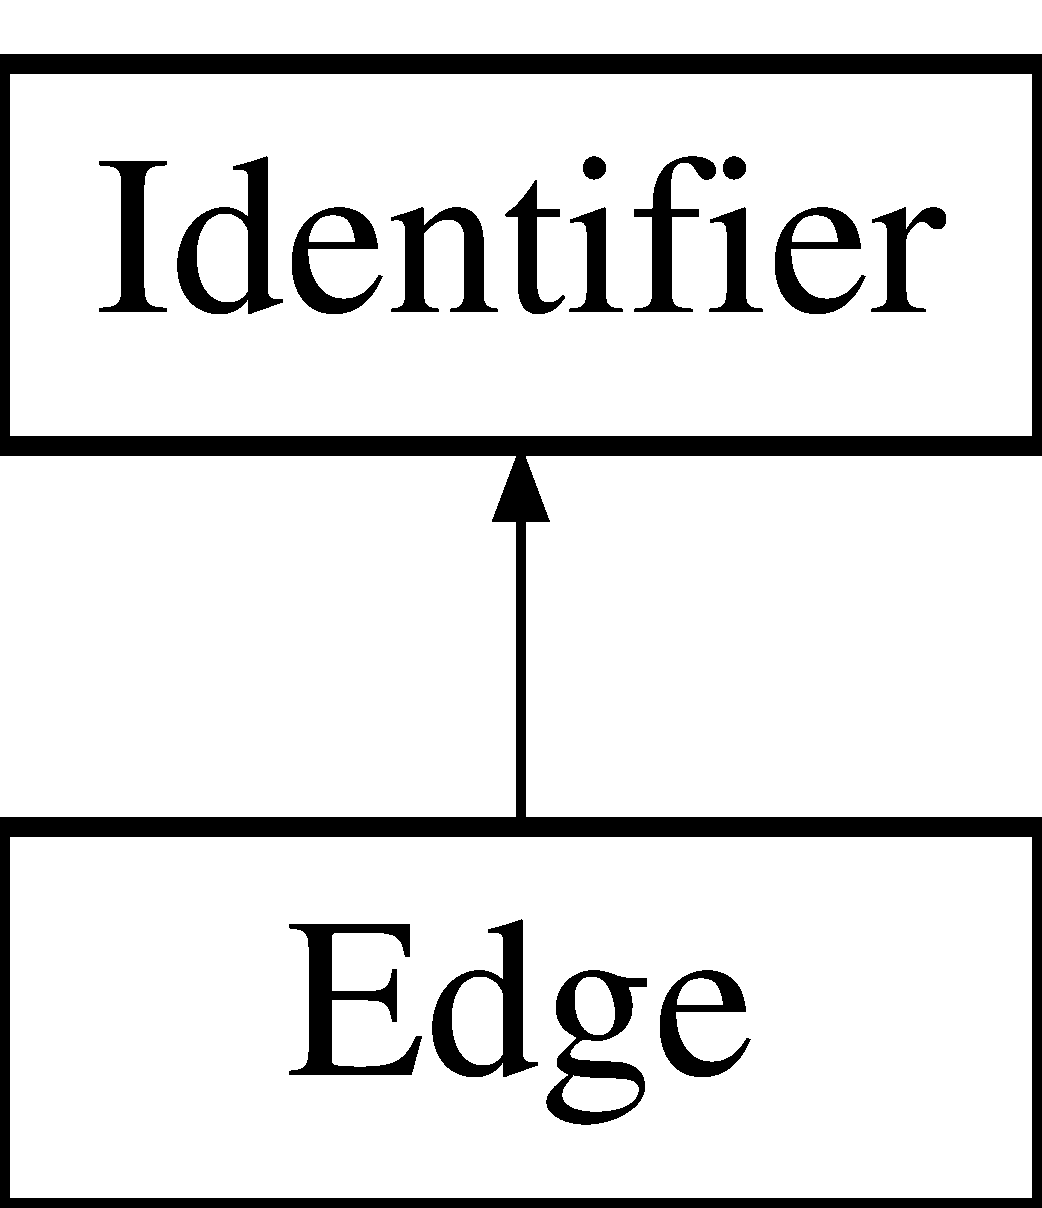
\includegraphics[height=2cm]{classEdge}
\end{center}
\end{figure}
\subsection*{Public Member Functions}
\begin{DoxyCompactItemize}
\item 
\hypertarget{classEdge_ab4cc26a850f41458630352cdba59d6b0}{
{\bfseries Edge} (Id id, BcId bcId, const \hyperlink{classPoint}{Point} \&start, const \hyperlink{classPoint}{Point} \&end)}
\label{classEdge_ab4cc26a850f41458630352cdba59d6b0}

\item 
\hypertarget{classEdge_af8d0a024ae2b1d02144c744140fe0285}{
void {\bfseries print} (std::ostream \&out) const }
\label{classEdge_af8d0a024ae2b1d02144c744140fe0285}

\item 
\hypertarget{classEdge_a2e750308a1b56fb5b17ca13136730ae7}{
\hyperlink{classPoint}{Point} {\bfseries getFirst} () const }
\label{classEdge_a2e750308a1b56fb5b17ca13136730ae7}

\item 
\hypertarget{classEdge_ae06457bc71fac7a58b35db0ea62a85ca}{
\hyperlink{classPoint}{Point} {\bfseries getEnd} () const }
\label{classEdge_ae06457bc71fac7a58b35db0ea62a85ca}

\item 
\hypertarget{classEdge_a1c6c3568ea4329c91674d6466311db9d}{
\hyperlink{classPoint}{Point} {\bfseries operator\mbox{[}$\,$\mbox{]}} (UInt i) const }
\label{classEdge_a1c6c3568ea4329c91674d6466311db9d}

\end{DoxyCompactItemize}
\subsection*{Static Public Attributes}
\begin{DoxyCompactItemize}
\item 
\hypertarget{classEdge_a77f401000ef6b1c32dd07f66e12c28f8}{
static const UInt {\bfseries NNODES} = 2}
\label{classEdge_a77f401000ef6b1c32dd07f66e12c28f8}

\item 
\hypertarget{classEdge_a11c1f025b24fb0b0b83da5ecd990eea0}{
static const UInt {\bfseries numSides} = 1}
\label{classEdge_a11c1f025b24fb0b0b83da5ecd990eea0}

\item 
\hypertarget{classEdge_af57901544ca809e56b0ef5517565f01a}{
static const UInt {\bfseries myDim} = 1}
\label{classEdge_af57901544ca809e56b0ef5517565f01a}

\end{DoxyCompactItemize}


\subsection{Detailed Description}
This class implements an \hyperlink{classEdge}{Edge}, as an objects composed by two 2D points. 

The documentation for this class was generated from the following files:\begin{DoxyCompactItemize}
\item 
src/mesh\_\-objects.hpp\item 
src/mesh\_\-objects.cpp\end{DoxyCompactItemize}

\hypertarget{structevent}{
\section{event Struct Reference}
\label{structevent}\index{event@{event}}
}
\subsection*{Public Attributes}
\begin{DoxyCompactItemize}
\item 
\hypertarget{structevent_ae976e470131f6f58fca02dd6159f341a}{
TRIREAL {\bfseries xkey}}
\label{structevent_ae976e470131f6f58fca02dd6159f341a}

\item 
\hypertarget{structevent_ae6ca98fcd6f2332cb4ee63c8f0899fb8}{
TRIREAL {\bfseries ykey}}
\label{structevent_ae6ca98fcd6f2332cb4ee63c8f0899fb8}

\item 
\hypertarget{structevent_ae5fd20373d30ff0819348af30beb33f3}{
VOID $\ast$ {\bfseries eventptr}}
\label{structevent_ae5fd20373d30ff0819348af30beb33f3}

\item 
\hypertarget{structevent_a9ff72d28ddb7ea57df47fe9f0a7e9004}{
int {\bfseries heapposition}}
\label{structevent_a9ff72d28ddb7ea57df47fe9f0a7e9004}

\end{DoxyCompactItemize}


The documentation for this struct was generated from the following file:\begin{DoxyCompactItemize}
\item 
src/triangle.c\end{DoxyCompactItemize}

\hypertarget{structflipstacker}{
\section{flipstacker Struct Reference}
\label{structflipstacker}\index{flipstacker@{flipstacker}}
}
\subsection*{Public Attributes}
\begin{DoxyCompactItemize}
\item 
\hypertarget{structflipstacker_af476effffe8e2f8f2af7108d0f18e7c7}{
triangle {\bfseries flippedtri}}
\label{structflipstacker_af476effffe8e2f8f2af7108d0f18e7c7}

\item 
\hypertarget{structflipstacker_aab8edb201c23d9f1d7955950f341230d}{
struct \hyperlink{structflipstacker}{flipstacker} $\ast$ {\bfseries prevflip}}
\label{structflipstacker_aab8edb201c23d9f1d7955950f341230d}

\end{DoxyCompactItemize}


The documentation for this struct was generated from the following file:\begin{DoxyCompactItemize}
\item 
src/triangle.c\end{DoxyCompactItemize}

\hypertarget{classHeader}{
\section{Header Class Reference}
\label{classHeader}\index{Header@{Header}}
}


It contains general information about the tree.  


{\ttfamily \#include $<$tree\_\-header.hpp$>$}

\subsection{Detailed Description}
It contains general information about the tree. 
\begin{DoxyParams}{Parameters}
\item[{\em T}]The template parameter expresses the original objects for the construction of the tree, it is used to store \hyperlink{classDomain}{Domain$<$T$>$}, T::dp() gives the physical dimension of the object and T::dt() gives the search dimension \par
 the tree always store Box$<$NDIMP$>$ and the index to find the original object (triangle...), if we want to store point we have to create a box from point (for example repeating the same coordinates for Min\_\-point and Max\_\-point) in the simplest case, or to change the structure adding the poin case everywhere (treenode...)\end{DoxyParams}
Default copy constructor and default destructor work fine. 

The documentation for this class was generated from the following file:\begin{DoxyCompactItemize}
\item 
src/\hyperlink{tree__header_8hpp}{tree\_\-header.hpp}\end{DoxyCompactItemize}

\hypertarget{classIdentifier}{
\section{Identifier Class Reference}
\label{classIdentifier}\index{Identifier@{Identifier}}
}


This class gives some common methods to all \hyperlink{structmesh}{mesh} objects.  


{\ttfamily \#include $<$mesh\_\-objects.hpp$>$}Inheritance diagram for Identifier::\begin{figure}[H]
\begin{center}
\leavevmode
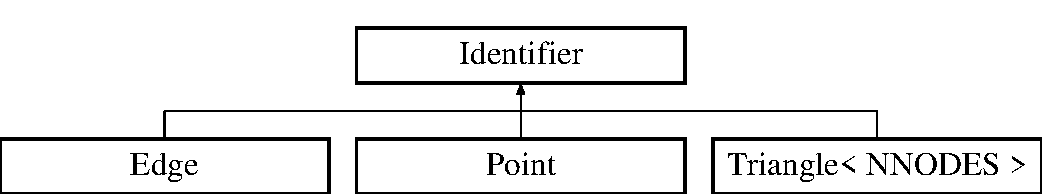
\includegraphics[height=2cm]{classIdentifier}
\end{center}
\end{figure}
\subsection*{Public Member Functions}
\begin{DoxyCompactItemize}
\item 
\hypertarget{classIdentifier_a681904976f9d3c8b7ea728ad1ea7778e}{
{\bfseries Identifier} (UInt id)}
\label{classIdentifier_a681904976f9d3c8b7ea728ad1ea7778e}

\item 
\hypertarget{classIdentifier_a75ddf5e6a39bf767bb4b275af581b638}{
{\bfseries Identifier} (UInt id, UInt bcId)}
\label{classIdentifier_a75ddf5e6a39bf767bb4b275af581b638}

\item 
\hypertarget{classIdentifier_a58f26c5c63f5683e6bfe9aa1dce6cc5b}{
bool {\bfseries unassignedId} () const }
\label{classIdentifier_a58f26c5c63f5683e6bfe9aa1dce6cc5b}

\item 
\hypertarget{classIdentifier_affb22acd31bc98b94246cac539654682}{
bool {\bfseries unassignedBc} () const }
\label{classIdentifier_affb22acd31bc98b94246cac539654682}

\item 
\hypertarget{classIdentifier_a2ab7d66987f46ab6bbbd78c7ea11e000}{
Id {\bfseries id} () const }
\label{classIdentifier_a2ab7d66987f46ab6bbbd78c7ea11e000}

\item 
\hypertarget{classIdentifier_acc353bc402ec82e6e507b0b3e447c938}{
BcId {\bfseries bcId} () const }
\label{classIdentifier_acc353bc402ec82e6e507b0b3e447c938}

\item 
\hypertarget{classIdentifier_a287f4ccdfdaac69cd5c7f6c68be5c6b1}{
Id {\bfseries getId} () const }
\label{classIdentifier_a287f4ccdfdaac69cd5c7f6c68be5c6b1}

\end{DoxyCompactItemize}
\subsection*{Static Public Attributes}
\begin{DoxyCompactItemize}
\item 
static const UInt \hyperlink{classIdentifier_a997af66122aaa17d73db9fe9bf9bdf71}{NVAL} = std::numeric\_\-limits$<$UInt$>$::max()
\begin{DoxyCompactList}\small\item\em An static const Unisgned Integer. \item\end{DoxyCompactList}\end{DoxyCompactItemize}
\subsection*{Protected Attributes}
\begin{DoxyCompactItemize}
\item 
\hypertarget{classIdentifier_a97c8576c0d08149eb3c743d9c74082e5}{
Id {\bfseries id\_\-}}
\label{classIdentifier_a97c8576c0d08149eb3c743d9c74082e5}

\item 
\hypertarget{classIdentifier_a946c44b08eb47d3e380a6c72f3f44370}{
BcId {\bfseries bcId\_\-}}
\label{classIdentifier_a946c44b08eb47d3e380a6c72f3f44370}

\end{DoxyCompactItemize}


\subsection{Detailed Description}
This class gives some common methods to all \hyperlink{structmesh}{mesh} objects. 

\subsection{Member Data Documentation}
\hypertarget{classIdentifier_a997af66122aaa17d73db9fe9bf9bdf71}{
\index{Identifier@{Identifier}!NVAL@{NVAL}}
\index{NVAL@{NVAL}!Identifier@{Identifier}}
\subsubsection[{NVAL}]{\setlength{\rightskip}{0pt plus 5cm}const UInt {\bf Identifier::NVAL} = std::numeric\_\-limits$<$UInt$>$::max()\hspace{0.3cm}{\ttfamily  \mbox{[}static\mbox{]}}}}
\label{classIdentifier_a997af66122aaa17d73db9fe9bf9bdf71}


An static const Unisgned Integer. Needed to identify the Not Valid Id. 

The documentation for this class was generated from the following files:\begin{DoxyCompactItemize}
\item 
src/mesh\_\-objects.hpp\item 
src/mesh\_\-objects.cpp\end{DoxyCompactItemize}

\hypertarget{classIOHandler}{
\section{IOHandler Class Reference}
\label{classIOHandler}\index{IOHandler@{IOHandler}}
}


An IO handler class for objects passed from R.  


{\ttfamily \#include $<$IO\_\-handler\_\-old.hpp$>$}\subsection*{Public Member Functions}
\begin{DoxyCompactItemize}
\item 
\hyperlink{classIOHandler_ab29ae5702f6c5238cc0e33a84625e709}{IOHandler} (VectorXr \&observations, MatrixXr \&design\_\-matrix, UInt order, Real lambda, std::vector$<$ UInt $>$ \&dirichlet\_\-indexes, std::vector$<$ Real $>$ \&dirichlet\_\-values)
\begin{DoxyCompactList}\small\item\em A basic version of the constructor. \item\end{DoxyCompactList}\item 
void \hyperlink{classIOHandler_ae1902fae16f3d44a15b76e175d2a7299}{printObservations} (std::ostream \&out)
\begin{DoxyCompactList}\small\item\em A complete version of the constructor. \item\end{DoxyCompactList}\item 
\hypertarget{classIOHandler_a181d9429c3de322d9b3782af0fdc2a2a}{
void {\bfseries printDesignMatrix} (std::ostream \&out)}
\label{classIOHandler_a181d9429c3de322d9b3782af0fdc2a2a}

\item 
\hypertarget{classIOHandler_a6e7ae9ae99f678c01e9c64dc1beda12a}{
void {\bfseries printLocations} (std::ostream \&out)}
\label{classIOHandler_a6e7ae9ae99f678c01e9c64dc1beda12a}

\item 
\hypertarget{classIOHandler_ae4519801e2879296dd3c906edb18afbd}{
VectorXr const \& \hyperlink{classIOHandler_ae4519801e2879296dd3c906edb18afbd}{getObservations} () const }
\label{classIOHandler_ae4519801e2879296dd3c906edb18afbd}

\begin{DoxyCompactList}\small\item\em A method returning a reference to the observations vector. \item\end{DoxyCompactList}\item 
\hypertarget{classIOHandler_a3dce10d31729949d19f234ea57a01844}{
MatrixXr const \& \hyperlink{classIOHandler_a3dce10d31729949d19f234ea57a01844}{getDesignMatrix} () const }
\label{classIOHandler_a3dce10d31729949d19f234ea57a01844}

\begin{DoxyCompactList}\small\item\em A method returning a reference to the design matrix. \item\end{DoxyCompactList}\item 
\hypertarget{classIOHandler_a3f4f820ee195e346d8c2dd8f202fb793}{
UInt const \hyperlink{classIOHandler_a3f4f820ee195e346d8c2dd8f202fb793}{getNumberofObservations} () const }
\label{classIOHandler_a3f4f820ee195e346d8c2dd8f202fb793}

\begin{DoxyCompactList}\small\item\em A method returning the number of observations. \item\end{DoxyCompactList}\item 
\hypertarget{classIOHandler_a9253260fd1c2d2a49a2ccb2e9bf307d3}{
std::vector$<$ \hyperlink{classPoint}{Point} $>$ const \& \hyperlink{classIOHandler_a9253260fd1c2d2a49a2ccb2e9bf307d3}{getLocations} () const }
\label{classIOHandler_a9253260fd1c2d2a49a2ccb2e9bf307d3}

\begin{DoxyCompactList}\small\item\em A method returning the locations of the observations. \item\end{DoxyCompactList}\item 
\hypertarget{classIOHandler_acfc1009b604200966d48031e21b71a4a}{
Real const \hyperlink{classIOHandler_acfc1009b604200966d48031e21b71a4a}{getLambda} () const }
\label{classIOHandler_acfc1009b604200966d48031e21b71a4a}

\begin{DoxyCompactList}\small\item\em A method returning the the penalization term. \item\end{DoxyCompactList}\item 
\hypertarget{classIOHandler_a5320d2bcb6513b607f4ef52325ab54ee}{
UInt const \hyperlink{classIOHandler_a5320d2bcb6513b607f4ef52325ab54ee}{getOrder} () const }
\label{classIOHandler_a5320d2bcb6513b607f4ef52325ab54ee}

\begin{DoxyCompactList}\small\item\em A method returning the input order. \item\end{DoxyCompactList}\item 
\hypertarget{classIOHandler_afacd04bc564b21e3baff7a5a73f3eb19}{
Real const \hyperlink{classIOHandler_afacd04bc564b21e3baff7a5a73f3eb19}{getC} () const }
\label{classIOHandler_afacd04bc564b21e3baff7a5a73f3eb19}

\begin{DoxyCompactList}\small\item\em A method returning the locations of the observations. \item\end{DoxyCompactList}\item 
\hypertarget{classIOHandler_a2b018ad9b621214c4ab79149ff69c55b}{
std::vector$<$ Real $>$ const \& \hyperlink{classIOHandler_a2b018ad9b621214c4ab79149ff69c55b}{getBeta} () const }
\label{classIOHandler_a2b018ad9b621214c4ab79149ff69c55b}

\begin{DoxyCompactList}\small\item\em A method returning the transport coefficient term. \item\end{DoxyCompactList}\item 
\hypertarget{classIOHandler_a6f22b7d632d5e0bd5ab8cc5d979b4e9a}{
Eigen::Matrix$<$ Real, 2, 2 $>$ const \& \hyperlink{classIOHandler_a6f22b7d632d5e0bd5ab8cc5d979b4e9a}{getK} () const }
\label{classIOHandler_a6f22b7d632d5e0bd5ab8cc5d979b4e9a}

\begin{DoxyCompactList}\small\item\em A method returning the matrix with unisotropic diffusion coefficients. \item\end{DoxyCompactList}\item 
\hypertarget{classIOHandler_a1f83ec53438b95513a8bce194de0d6db}{
VectorXr const \& \hyperlink{classIOHandler_a1f83ec53438b95513a8bce194de0d6db}{getU} () const }
\label{classIOHandler_a1f83ec53438b95513a8bce194de0d6db}

\begin{DoxyCompactList}\small\item\em A method returning the integrals of the forcing term. \item\end{DoxyCompactList}\item 
\hypertarget{classIOHandler_a9e42ef3bedfb3d4af2b6d8d1b151e94e}{
std::vector$<$ UInt $>$ const \& \hyperlink{classIOHandler_a9e42ef3bedfb3d4af2b6d8d1b151e94e}{getDirichletIndexes} () const }
\label{classIOHandler_a9e42ef3bedfb3d4af2b6d8d1b151e94e}

\begin{DoxyCompactList}\small\item\em A method returning the indexes of the nodes for which is needed to apply Dirichlet Conditions. \item\end{DoxyCompactList}\item 
\hypertarget{classIOHandler_a6939535198d0550bd1b07aac82b6c421}{
std::vector$<$ Real $>$ const \& \hyperlink{classIOHandler_a6939535198d0550bd1b07aac82b6c421}{getDirichletValues} () const }
\label{classIOHandler_a6939535198d0550bd1b07aac82b6c421}

\begin{DoxyCompactList}\small\item\em A method returning the values to apply for Dirichlet Conditions. \item\end{DoxyCompactList}\end{DoxyCompactItemize}


\subsection{Detailed Description}
An IO handler class for objects passed from R. This class, given the data from R, convert them in a C++ format, offering a series of method for their access, so isolating the more the possible the specific code for R/C++ data conversion. 

\subsection{Constructor \& Destructor Documentation}
\hypertarget{classIOHandler_ab29ae5702f6c5238cc0e33a84625e709}{
\index{IOHandler@{IOHandler}!IOHandler@{IOHandler}}
\index{IOHandler@{IOHandler}!IOHandler@{IOHandler}}
\subsubsection[{IOHandler}]{\setlength{\rightskip}{0pt plus 5cm}IOHandler::IOHandler (VectorXr \& {\em observations}, \/  MatrixXr \& {\em design\_\-matrix}, \/  UInt {\em order}, \/  Real {\em lambda}, \/  std::vector$<$ UInt $>$ \& {\em dirichlet\_\-indexes}, \/  std::vector$<$ Real $>$ \& {\em dirichlet\_\-values})\hspace{0.3cm}{\ttfamily  \mbox{[}inline\mbox{]}}}}
\label{classIOHandler_ab29ae5702f6c5238cc0e33a84625e709}


A basic version of the constructor. It initializes the object storing the R given objects. This is the simplest of the two possible interfaces with R 
\begin{DoxyParams}{Parameters}
\item[{\em Robservations}]an R-\/vector containing the values of the observations. \item[{\em Rdesmat}]an R-\/matrix containing the design matrix for the regression. \item[{\em Rorder}]an R-\/integer containing the order of the approximating basis. \item[{\em Rlambda}]an R-\/double containing the penalization term of the empirical evidence respect to the prior one. \item[{\em Rbindex}]an R-\/integer containing the indexes of the nodes the user want to apply a Dirichlet Condition, the other are automatically considered in Neumann Condition. \item[{\em Rbvalues}]an R-\/double containing the value to impose for the Dirichlet condition, on the indexes specified in Rbindex \end{DoxyParams}


\subsection{Member Function Documentation}
\hypertarget{classIOHandler_ae1902fae16f3d44a15b76e175d2a7299}{
\index{IOHandler@{IOHandler}!printObservations@{printObservations}}
\index{printObservations@{printObservations}!IOHandler@{IOHandler}}
\subsubsection[{printObservations}]{\setlength{\rightskip}{0pt plus 5cm}void IOHandler::printObservations (std::ostream \& {\em out})}}
\label{classIOHandler_ae1902fae16f3d44a15b76e175d2a7299}


A complete version of the constructor. It initializes the object storing the R given objects. This is the simplest of the two possible interfaces with R 
\begin{DoxyParams}{Parameters}
\item[{\em Robservations}]an R-\/vector containing the values of the observations. \item[{\em Rdesmat}]an R-\/matrix containing the design matrix for the regression. \item[{\em Rorder}]an R-\/integer containing the order of the approximating basis. \item[{\em Rlambda}]an R-\/double containing the penalization term of the empirical evidence respect to the prior one. \item[{\em Rbindex}]an R-\/integer vector containing the indexes of the nodes the user want to apply a Dirichlet Condition, the other are automatically considered in Neumann Condition. \item[{\em Rbvalues}]an R-\/double vector containing the value to impose for the Dirichlet condition, on the indexes specified in Rbindex \item[{\em Rc}]an R-\/double that contains the coefficient of the REACTION term \item[{\em Rbeta}]an R-\/double 2-\/dim vector that contains the coefficients for the TRANSPORT coefficients. \item[{\em RK}]an R-\/double 2X2 matrix containing the coefficients for a anisotropic DIFFUSION term. \item[{\em (UNSUPPORTED}]put it zero) Ru an R-\/double vector of length triangles that contaiins the forcing term integrals. \end{DoxyParams}


The documentation for this class was generated from the following files:\begin{DoxyCompactItemize}
\item 
src/IO\_\-handler\_\-old.hpp\item 
src/IO\_\-handler\_\-imp\_\-old.hpp\end{DoxyCompactItemize}

\hypertarget{classLevRuntimeError}{
\section{LevRuntimeError$<$ Shape $>$ Class Template Reference}
\label{classLevRuntimeError}\index{LevRuntimeError@{LevRuntimeError}}
}


This class is used to report an attempt to build a tree with more levels than a fixed limit.  


{\ttfamily \#include $<$exception\_\-handling.hpp$>$}Inheritance diagram for LevRuntimeError$<$ Shape $>$::\begin{figure}[H]
\begin{center}
\leavevmode
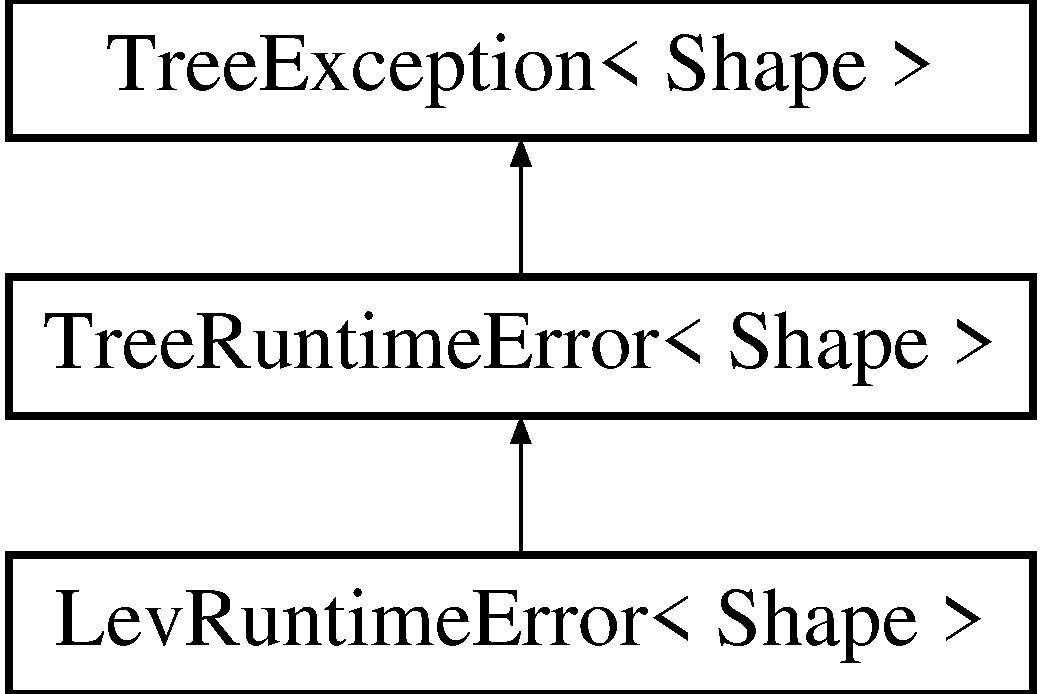
\includegraphics[height=3cm]{classLevRuntimeError}
\end{center}
\end{figure}
\subsection*{Static Public Member Functions}
\begin{DoxyCompactItemize}
\item 
\hypertarget{classLevRuntimeError_a9b99f52a1fabe68b2abf6e59cc07d516}{
static void \hyperlink{classLevRuntimeError_a9b99f52a1fabe68b2abf6e59cc07d516}{setmaxtreelev} (int const \&mlev)}
\label{classLevRuntimeError_a9b99f52a1fabe68b2abf6e59cc07d516}

\begin{DoxyCompactList}\small\item\em Sets the maximum number of tree levels. \item\end{DoxyCompactList}\item 
\hypertarget{classLevRuntimeError_a47cd6be3db2365778750b7e70d37b4a5}{
static int \hyperlink{classLevRuntimeError_a47cd6be3db2365778750b7e70d37b4a5}{getmaxtreelev} ()}
\label{classLevRuntimeError_a47cd6be3db2365778750b7e70d37b4a5}

\begin{DoxyCompactList}\small\item\em Gets the maximum number of tree levels. \item\end{DoxyCompactList}\end{DoxyCompactItemize}
\subsection*{Static Protected Attributes}
\begin{DoxyCompactItemize}
\item 
\hypertarget{classLevRuntimeError_a059c75733530dac291cd5eef1b204b81}{
static int \hyperlink{classLevRuntimeError_a059c75733530dac291cd5eef1b204b81}{max\_\-tree\_\-lev} = 1.e3}
\label{classLevRuntimeError_a059c75733530dac291cd5eef1b204b81}

\begin{DoxyCompactList}\small\item\em Maximum tree levels. \item\end{DoxyCompactList}\end{DoxyCompactItemize}


\subsection{Detailed Description}
\subsubsection*{template$<$class Shape$>$ class LevRuntimeError$<$ Shape $>$}

This class is used to report an attempt to build a tree with more levels than a fixed limit. 

The documentation for this class was generated from the following file:\begin{DoxyCompactItemize}
\item 
src/\hyperlink{exception__handling_8hpp}{exception\_\-handling.hpp}\end{DoxyCompactItemize}

\hypertarget{classLocLengthError}{
\section{LocLengthError$<$ Shape $>$ Class Template Reference}
\label{classLocLengthError}\index{LocLengthError@{LocLengthError}}
}


This class is used to report an attempt to build a tree with more memory locations than a fixed limit.  


{\ttfamily \#include $<$exception\_\-handling.hpp$>$}Inheritance diagram for LocLengthError$<$ Shape $>$::\begin{figure}[H]
\begin{center}
\leavevmode
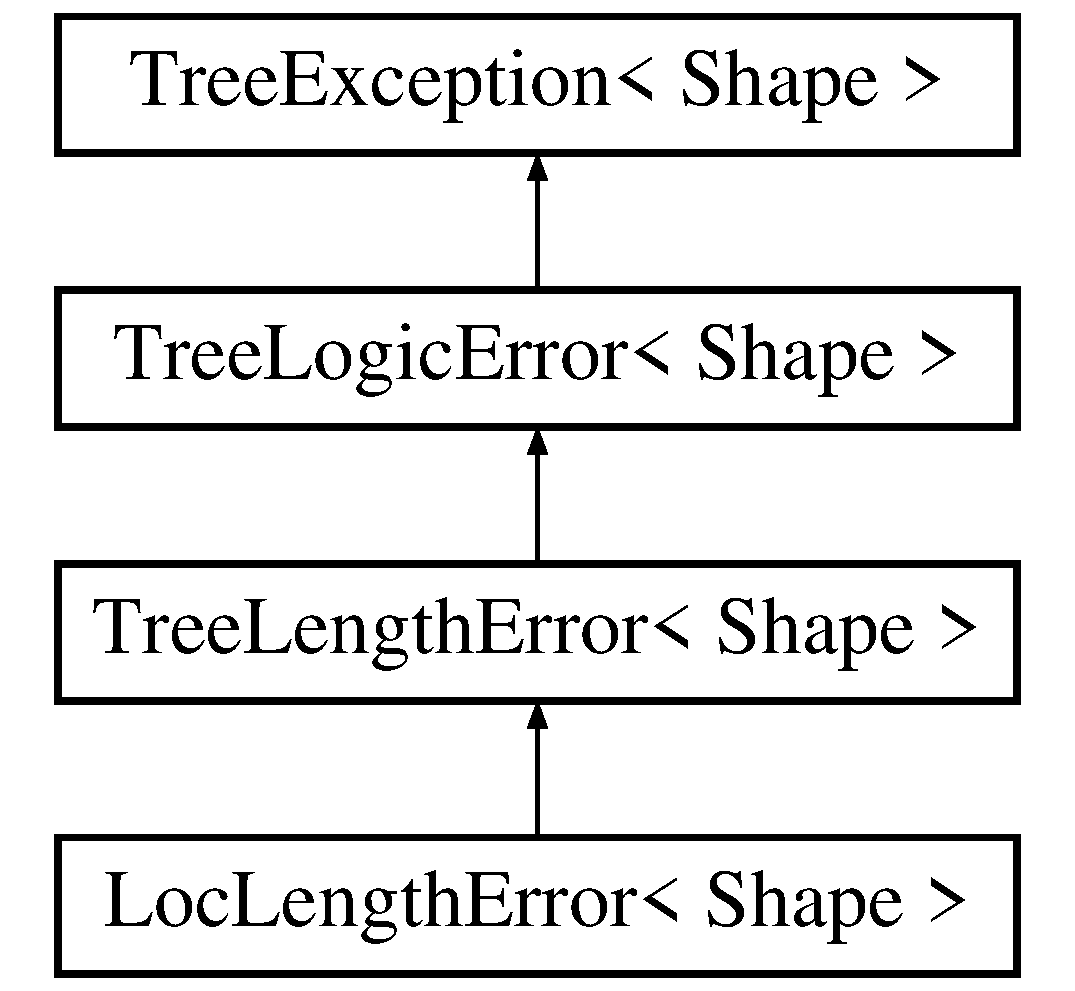
\includegraphics[height=4cm]{classLocLengthError}
\end{center}
\end{figure}
\subsection*{Public Member Functions}
\begin{DoxyCompactItemize}
\item 
\hyperlink{classLocLengthError_aa99b1f424fc5d9a081269f99ea239230}{LocLengthError} (int const \&mtree, int const \&ntree)
\item 
\hypertarget{classLocLengthError_add45b8c75237409ce118719cc668473b}{
int const \hyperlink{classLocLengthError_add45b8c75237409ce118719cc668473b}{getmaxtreeloc} () const }
\label{classLocLengthError_add45b8c75237409ce118719cc668473b}

\begin{DoxyCompactList}\small\item\em Gets the maximum number of tree memory locations available. \item\end{DoxyCompactList}\item 
\hypertarget{classLocLengthError_a35bc168775794537fe7ffae95c2af138}{
int const \hyperlink{classLocLengthError_a35bc168775794537fe7ffae95c2af138}{gettreeloc} () const }
\label{classLocLengthError_a35bc168775794537fe7ffae95c2af138}

\begin{DoxyCompactList}\small\item\em Gets the number of tree memory locations needed. \item\end{DoxyCompactList}\end{DoxyCompactItemize}
\subsection*{Protected Attributes}
\begin{DoxyCompactItemize}
\item 
\hypertarget{classLocLengthError_aae1abb4777cbb5be258a7349ff1cc30f}{
int \hyperlink{classLocLengthError_aae1abb4777cbb5be258a7349ff1cc30f}{max\_\-tree\_\-loc}}
\label{classLocLengthError_aae1abb4777cbb5be258a7349ff1cc30f}

\begin{DoxyCompactList}\small\item\em Maximum tree memory locations available. \item\end{DoxyCompactList}\item 
\hypertarget{classLocLengthError_afe2db13de26663e929ecf1ed2839adef}{
int \hyperlink{classLocLengthError_afe2db13de26663e929ecf1ed2839adef}{tree\_\-loc}}
\label{classLocLengthError_afe2db13de26663e929ecf1ed2839adef}

\begin{DoxyCompactList}\small\item\em Tree memory locations needed. \item\end{DoxyCompactList}\end{DoxyCompactItemize}


\subsection{Detailed Description}
\subsubsection*{template$<$class Shape$>$ class LocLengthError$<$ Shape $>$}

This class is used to report an attempt to build a tree with more memory locations than a fixed limit. 

\subsection{Constructor \& Destructor Documentation}
\hypertarget{classLocLengthError_aa99b1f424fc5d9a081269f99ea239230}{
\index{LocLengthError@{LocLengthError}!LocLengthError@{LocLengthError}}
\index{LocLengthError@{LocLengthError}!LocLengthError@{LocLengthError}}
\subsubsection[{LocLengthError}]{\setlength{\rightskip}{0pt plus 5cm}template$<$class Shape$>$ {\bf LocLengthError}$<$ Shape $>$::{\bf LocLengthError} (int const \& {\em mtree}, \/  int const \& {\em ntree})\hspace{0.3cm}{\ttfamily  \mbox{[}inline\mbox{]}}}}
\label{classLocLengthError_aa99b1f424fc5d9a081269f99ea239230}
A constructor.

Initialize the number of the required tree locations. 

The documentation for this class was generated from the following file:\begin{DoxyCompactItemize}
\item 
src/\hyperlink{exception__handling_8hpp}{exception\_\-handling.hpp}\end{DoxyCompactItemize}

\hypertarget{structmemorypool}{
\section{memorypool Struct Reference}
\label{structmemorypool}\index{memorypool@{memorypool}}
}
\subsection*{Public Attributes}
\begin{DoxyCompactItemize}
\item 
\hypertarget{structmemorypool_afac6d33dcfe9df284f27ca630123332f}{
VOID $\ast$$\ast$ {\bfseries firstblock}}
\label{structmemorypool_afac6d33dcfe9df284f27ca630123332f}

\item 
\hypertarget{structmemorypool_aaf9ecf13c92d2bfbf3bcbfb8715e19f0}{
VOID $\ast$$\ast$ {\bfseries nowblock}}
\label{structmemorypool_aaf9ecf13c92d2bfbf3bcbfb8715e19f0}

\item 
\hypertarget{structmemorypool_a998808704144a4045a7e03656ef94185}{
VOID $\ast$ {\bfseries nextitem}}
\label{structmemorypool_a998808704144a4045a7e03656ef94185}

\item 
\hypertarget{structmemorypool_a994ac2f58b146dc4eaef504a70358582}{
VOID $\ast$ {\bfseries deaditemstack}}
\label{structmemorypool_a994ac2f58b146dc4eaef504a70358582}

\item 
\hypertarget{structmemorypool_a72733c1e19035f973e60706be7b32364}{
VOID $\ast$$\ast$ {\bfseries pathblock}}
\label{structmemorypool_a72733c1e19035f973e60706be7b32364}

\item 
\hypertarget{structmemorypool_a60cac87ccd6a441c5358a5bf9fcf3064}{
VOID $\ast$ {\bfseries pathitem}}
\label{structmemorypool_a60cac87ccd6a441c5358a5bf9fcf3064}

\item 
\hypertarget{structmemorypool_a143c77d997e424a4be406ee4b3338c12}{
int {\bfseries alignbytes}}
\label{structmemorypool_a143c77d997e424a4be406ee4b3338c12}

\item 
\hypertarget{structmemorypool_a2658208bb7b2949b51f679e0a8278e3b}{
int {\bfseries itembytes}}
\label{structmemorypool_a2658208bb7b2949b51f679e0a8278e3b}

\item 
\hypertarget{structmemorypool_a725760a5cc69917ea955ce4b64ed022f}{
int {\bfseries itemsperblock}}
\label{structmemorypool_a725760a5cc69917ea955ce4b64ed022f}

\item 
\hypertarget{structmemorypool_aea58af830e899435d7f9547fd8920c3f}{
int {\bfseries itemsfirstblock}}
\label{structmemorypool_aea58af830e899435d7f9547fd8920c3f}

\item 
\hypertarget{structmemorypool_a9a59491a2dbbb46ae00b494a2652404f}{
long {\bfseries items}}
\label{structmemorypool_a9a59491a2dbbb46ae00b494a2652404f}

\item 
\hypertarget{structmemorypool_a851a3bc61c20c58ba0da9b8e45e7ab3d}{
long {\bfseries maxitems}}
\label{structmemorypool_a851a3bc61c20c58ba0da9b8e45e7ab3d}

\item 
\hypertarget{structmemorypool_ae407db4294305e97b4072f6117f2bfa9}{
int {\bfseries unallocateditems}}
\label{structmemorypool_ae407db4294305e97b4072f6117f2bfa9}

\item 
\hypertarget{structmemorypool_a34c47ac30b534652a93e9d3f742648ff}{
int {\bfseries pathitemsleft}}
\label{structmemorypool_a34c47ac30b534652a93e9d3f742648ff}

\end{DoxyCompactItemize}


The documentation for this struct was generated from the following file:\begin{DoxyCompactItemize}
\item 
src/triangle.c\end{DoxyCompactItemize}

\hypertarget{structmesh}{
\section{mesh Struct Reference}
\label{structmesh}\index{mesh@{mesh}}
}
\subsection*{Public Attributes}
\begin{DoxyCompactItemize}
\item 
\hypertarget{structmesh_a69079626a8de35998ff5ee644aeb5b5a}{
struct \hyperlink{structmemorypool}{memorypool} {\bfseries triangles}}
\label{structmesh_a69079626a8de35998ff5ee644aeb5b5a}

\item 
\hypertarget{structmesh_a3c29f7e745ae22b5bb4cf08d49b77895}{
struct \hyperlink{structmemorypool}{memorypool} {\bfseries subsegs}}
\label{structmesh_a3c29f7e745ae22b5bb4cf08d49b77895}

\item 
\hypertarget{structmesh_a9812ee57bbbb5b168d4a85403e5acbad}{
struct \hyperlink{structmemorypool}{memorypool} {\bfseries vertices}}
\label{structmesh_a9812ee57bbbb5b168d4a85403e5acbad}

\item 
\hypertarget{structmesh_a3cb8300dd2e6dc4e11795ac178bf02b5}{
struct \hyperlink{structmemorypool}{memorypool} {\bfseries viri}}
\label{structmesh_a3cb8300dd2e6dc4e11795ac178bf02b5}

\item 
\hypertarget{structmesh_aeb8da45b7822882ee7db7d1a1249a0b7}{
struct \hyperlink{structmemorypool}{memorypool} {\bfseries badsubsegs}}
\label{structmesh_aeb8da45b7822882ee7db7d1a1249a0b7}

\item 
\hypertarget{structmesh_a05cf8b5d0015464c86521cd8a1ddd768}{
struct \hyperlink{structmemorypool}{memorypool} {\bfseries badtriangles}}
\label{structmesh_a05cf8b5d0015464c86521cd8a1ddd768}

\item 
\hypertarget{structmesh_a21056ea10e510d8aaa99e93d35ef5fe2}{
struct \hyperlink{structmemorypool}{memorypool} {\bfseries flipstackers}}
\label{structmesh_a21056ea10e510d8aaa99e93d35ef5fe2}

\item 
\hypertarget{structmesh_a86186d96a9bac08ba51665bce57a4009}{
struct \hyperlink{structmemorypool}{memorypool} {\bfseries splaynodes}}
\label{structmesh_a86186d96a9bac08ba51665bce57a4009}

\item 
\hypertarget{structmesh_a9fb6633c391887f9ece4f47c6251d806}{
struct \hyperlink{structbadtriang}{badtriang} $\ast$ {\bfseries queuefront} \mbox{[}4096\mbox{]}}
\label{structmesh_a9fb6633c391887f9ece4f47c6251d806}

\item 
\hypertarget{structmesh_a194e9c6cc034fe96c3eb3d6660e0d5d7}{
struct \hyperlink{structbadtriang}{badtriang} $\ast$ {\bfseries queuetail} \mbox{[}4096\mbox{]}}
\label{structmesh_a194e9c6cc034fe96c3eb3d6660e0d5d7}

\item 
\hypertarget{structmesh_a67dae9c18940347bff87ac492258acb5}{
int {\bfseries nextnonemptyq} \mbox{[}4096\mbox{]}}
\label{structmesh_a67dae9c18940347bff87ac492258acb5}

\item 
\hypertarget{structmesh_a420eac8320d421bf6ba4d68daef14107}{
int {\bfseries firstnonemptyq}}
\label{structmesh_a420eac8320d421bf6ba4d68daef14107}

\item 
\hypertarget{structmesh_a8a82d7821fd526fb8f406be1ece5b591}{
struct \hyperlink{structflipstacker}{flipstacker} $\ast$ {\bfseries lastflip}}
\label{structmesh_a8a82d7821fd526fb8f406be1ece5b591}

\item 
\hypertarget{structmesh_a69d1ecb3863a6a57919c1d7ac9251e21}{
TRIREAL {\bfseries xmin}}
\label{structmesh_a69d1ecb3863a6a57919c1d7ac9251e21}

\item 
\hypertarget{structmesh_a555362201efc9549764ec7f6a22b6095}{
TRIREAL {\bfseries xmax}}
\label{structmesh_a555362201efc9549764ec7f6a22b6095}

\item 
\hypertarget{structmesh_af999aedf5ee3137470c19dda98699ac7}{
TRIREAL {\bfseries ymin}}
\label{structmesh_af999aedf5ee3137470c19dda98699ac7}

\item 
\hypertarget{structmesh_ab887f178cdfb697b6b0ba1579ba5970a}{
TRIREAL {\bfseries ymax}}
\label{structmesh_ab887f178cdfb697b6b0ba1579ba5970a}

\item 
\hypertarget{structmesh_a569331804585352e603ac2f346a3cea6}{
TRIREAL {\bfseries xminextreme}}
\label{structmesh_a569331804585352e603ac2f346a3cea6}

\item 
\hypertarget{structmesh_a35525eea6ffd1d5614056308a7530666}{
int {\bfseries invertices}}
\label{structmesh_a35525eea6ffd1d5614056308a7530666}

\item 
\hypertarget{structmesh_a28f2e051b63158101968800794eab4e0}{
int {\bfseries inelements}}
\label{structmesh_a28f2e051b63158101968800794eab4e0}

\item 
\hypertarget{structmesh_a73c5f197d430325bb6ac23eed403c980}{
int {\bfseries insegments}}
\label{structmesh_a73c5f197d430325bb6ac23eed403c980}

\item 
\hypertarget{structmesh_a79d60900211b0af5134c7fe42dd63f2e}{
int {\bfseries holes}}
\label{structmesh_a79d60900211b0af5134c7fe42dd63f2e}

\item 
\hypertarget{structmesh_a32aa80933edcdeb91d9e4a5cb829d152}{
int {\bfseries regions}}
\label{structmesh_a32aa80933edcdeb91d9e4a5cb829d152}

\item 
\hypertarget{structmesh_abb122e5a5df3c10331505101836a1911}{
int {\bfseries undeads}}
\label{structmesh_abb122e5a5df3c10331505101836a1911}

\item 
\hypertarget{structmesh_a0cb925bd98331ef675e9d2d54451287b}{
long {\bfseries edges}}
\label{structmesh_a0cb925bd98331ef675e9d2d54451287b}

\item 
\hypertarget{structmesh_a041f090b1359b3f5400e2de065189dda}{
int {\bfseries mesh\_\-dim}}
\label{structmesh_a041f090b1359b3f5400e2de065189dda}

\item 
\hypertarget{structmesh_a9b7c4e029d2c5fb35f85a50e72cc7360}{
int {\bfseries nextras}}
\label{structmesh_a9b7c4e029d2c5fb35f85a50e72cc7360}

\item 
\hypertarget{structmesh_a169bb551d251dd98d70dc5fe56752ae7}{
int {\bfseries eextras}}
\label{structmesh_a169bb551d251dd98d70dc5fe56752ae7}

\item 
\hypertarget{structmesh_a42f62619f16224b639fc19e576760f12}{
long {\bfseries hullsize}}
\label{structmesh_a42f62619f16224b639fc19e576760f12}

\item 
\hypertarget{structmesh_a733d949838b84a6f3bb3db1249629d4d}{
int {\bfseries steinerleft}}
\label{structmesh_a733d949838b84a6f3bb3db1249629d4d}

\item 
\hypertarget{structmesh_ad26295d23d2acf33464c939537c0e992}{
int {\bfseries vertexmarkindex}}
\label{structmesh_ad26295d23d2acf33464c939537c0e992}

\item 
\hypertarget{structmesh_a5518ad2f754ab5f06311a0f92b6a39e4}{
int {\bfseries vertex2triindex}}
\label{structmesh_a5518ad2f754ab5f06311a0f92b6a39e4}

\item 
\hypertarget{structmesh_ab371a73d1a9dfe5e026bca7293c8e27f}{
int {\bfseries highorderindex}}
\label{structmesh_ab371a73d1a9dfe5e026bca7293c8e27f}

\item 
\hypertarget{structmesh_adf87a63b4bf9e70afb435d1394c3b31b}{
int {\bfseries elemattribindex}}
\label{structmesh_adf87a63b4bf9e70afb435d1394c3b31b}

\item 
\hypertarget{structmesh_ae8a2397a2bba31f9a3a5208aa4c4fff0}{
int {\bfseries areaboundindex}}
\label{structmesh_ae8a2397a2bba31f9a3a5208aa4c4fff0}

\item 
\hypertarget{structmesh_a8d2a76d3e90fac9e7839a99668f1669c}{
int {\bfseries checksegments}}
\label{structmesh_a8d2a76d3e90fac9e7839a99668f1669c}

\item 
\hypertarget{structmesh_acf6f25ff46f70f52500dd0b3dc3336ea}{
int {\bfseries checkquality}}
\label{structmesh_acf6f25ff46f70f52500dd0b3dc3336ea}

\item 
\hypertarget{structmesh_ab980847b749a285572fac285cb94c843}{
int {\bfseries readnodefile}}
\label{structmesh_ab980847b749a285572fac285cb94c843}

\item 
\hypertarget{structmesh_a2db40a26df07dfcb14c6bb5597b97e5b}{
long {\bfseries samples}}
\label{structmesh_a2db40a26df07dfcb14c6bb5597b97e5b}

\item 
\hypertarget{structmesh_a449675e549ebc9919410b310e568082e}{
long {\bfseries incirclecount}}
\label{structmesh_a449675e549ebc9919410b310e568082e}

\item 
\hypertarget{structmesh_a8d57c7f3b17990b5e3fc4ebc781e55f0}{
long {\bfseries counterclockcount}}
\label{structmesh_a8d57c7f3b17990b5e3fc4ebc781e55f0}

\item 
\hypertarget{structmesh_a07b2f99af7c405fe94a18c264a86a2d5}{
long {\bfseries orient3dcount}}
\label{structmesh_a07b2f99af7c405fe94a18c264a86a2d5}

\item 
\hypertarget{structmesh_ad846f50f4787288eef12a09a9c02cd54}{
long {\bfseries hyperbolacount}}
\label{structmesh_ad846f50f4787288eef12a09a9c02cd54}

\item 
\hypertarget{structmesh_a1ba65d762f34347b9f2dcb6f172636bd}{
long {\bfseries circumcentercount}}
\label{structmesh_a1ba65d762f34347b9f2dcb6f172636bd}

\item 
\hypertarget{structmesh_a9b54a570701c2bf248cf03438a1affc9}{
long {\bfseries circletopcount}}
\label{structmesh_a9b54a570701c2bf248cf03438a1affc9}

\item 
\hypertarget{structmesh_ac2d8384391395619b4dbda40b6bbddfd}{
vertex {\bfseries infvertex1}}
\label{structmesh_ac2d8384391395619b4dbda40b6bbddfd}

\item 
\hypertarget{structmesh_af1d3d858c7cbd4122b978143c0b08c4b}{
vertex {\bfseries infvertex2}}
\label{structmesh_af1d3d858c7cbd4122b978143c0b08c4b}

\item 
\hypertarget{structmesh_a530fa3d54ca3b95b34fbc233926ac185}{
vertex {\bfseries infvertex3}}
\label{structmesh_a530fa3d54ca3b95b34fbc233926ac185}

\item 
\hypertarget{structmesh_aeb2991e8af23a60d34462e28cd3881fb}{
triangle $\ast$ {\bfseries dummytri}}
\label{structmesh_aeb2991e8af23a60d34462e28cd3881fb}

\item 
\hypertarget{structmesh_a93c385f82ea2bf1c0d0b794824bef716}{
triangle $\ast$ {\bfseries dummytribase}}
\label{structmesh_a93c385f82ea2bf1c0d0b794824bef716}

\item 
\hypertarget{structmesh_ac3956fb994a62f704af23ceb16680ff8}{
subseg $\ast$ {\bfseries dummysub}}
\label{structmesh_ac3956fb994a62f704af23ceb16680ff8}

\item 
\hypertarget{structmesh_a5c152aa62e1ee91832c176920164c2a7}{
subseg $\ast$ {\bfseries dummysubbase}}
\label{structmesh_a5c152aa62e1ee91832c176920164c2a7}

\item 
\hypertarget{structmesh_a3fe1c34473c1475118c2253d7cafb17c}{
struct \hyperlink{structotri}{otri} {\bfseries recenttri}}
\label{structmesh_a3fe1c34473c1475118c2253d7cafb17c}

\end{DoxyCompactItemize}


The documentation for this struct was generated from the following file:\begin{DoxyCompactItemize}
\item 
src/triangle.c\end{DoxyCompactItemize}

\hypertarget{classMeshHandler}{
\section{MeshHandler$<$ ORDER $>$ Class Template Reference}
\label{classMeshHandler}\index{MeshHandler@{MeshHandler}}
}


This class gives an object-\/oriented reading interface to the output of the library \hyperlink{classTriangle}{Triangle} (Jonathan Richard Shewchuk).  


{\ttfamily \#include $<$mesh.hpp$>$}\subsection*{Public Types}
\begin{DoxyCompactItemize}
\item 
\hypertarget{classMeshHandler_ad644d0751db0969df9a4255750056f8f}{
typedef int {\bfseries UInt}}
\label{classMeshHandler_ad644d0751db0969df9a4255750056f8f}

\end{DoxyCompactItemize}
\subsection*{Public Member Functions}
\begin{DoxyCompactItemize}
\item 
\hyperlink{classMeshHandler_a983560a8f515c91a25a13d7d14b751c2}{MeshHandler} (Real $\ast$points, UInt $\ast$edges, UInt $\ast$triangles, UInt $\ast$neighbors, UInt num\_\-nodes, UInt num\_\-edges, UInt num\_\-triangles)
\begin{DoxyCompactList}\small\item\em A constructor. \item\end{DoxyCompactList}\item 
\hyperlink{classMeshHandler_a07339e31fd7550c9a9f8a99deba34074}{MeshHandler} (Real $\ast$points, UInt $\ast$edges, UInt $\ast$triangles, UInt $\ast$neighbors, UInt num\_\-nodes, UInt num\_\-edges, UInt num\_\-triangles, bool flag)
\begin{DoxyCompactList}\small\item\em Another constructor. \item\end{DoxyCompactList}\item 
UInt \hyperlink{classMeshHandler_aad0e450b97d6cf690d31b850524e7cda}{num\_\-nodes} () const 
\begin{DoxyCompactList}\small\item\em A normal member returning an unsigned integer value. \item\end{DoxyCompactList}\item 
UInt \hyperlink{classMeshHandler_a8c6a559cb5b5024d591c1edaa560a111}{num\_\-triangles} () const 
\begin{DoxyCompactList}\small\item\em A normal member returning an unsigned integer value. \item\end{DoxyCompactList}\item 
UInt \hyperlink{classMeshHandler_a545391eb9397b594ecbe0adae69a6887}{num\_\-edges} () const 
\begin{DoxyCompactList}\small\item\em A normal member returning an unsigned integer value. \item\end{DoxyCompactList}\item 
\hyperlink{classPoint}{Point} \hyperlink{classMeshHandler_a5657ecd9b4774575759ba816156e1586}{getPoint} (Id id)
\begin{DoxyCompactList}\small\item\em A normal member returning a \hyperlink{classPoint}{Point}. \item\end{DoxyCompactList}\item 
\hyperlink{classEdge}{Edge} \hyperlink{classMeshHandler_a346871cf4c2aa8082e81a76dd7ef5373}{getEdge} (Id id)
\begin{DoxyCompactList}\small\item\em A normal member returning an \hyperlink{classEdge}{Edge}. \item\end{DoxyCompactList}\item 
\hyperlink{classTriangle}{Triangle}$<$ ORDER $\ast$3 $>$ \hyperlink{classMeshHandler_affac7f7128b883d6a0a6cdd19c1bd9bd}{getTriangle} (Id id) const 
\begin{DoxyCompactList}\small\item\em A normal member returning a \hyperlink{classTriangle}{Triangle}. \item\end{DoxyCompactList}\item 
\hyperlink{classTriangle}{Triangle}$<$ ORDER $\ast$3 $>$ \hyperlink{classMeshHandler_a67e2b3d75d30094f0a5a8d72213bdca3}{getNeighbors} (Id id\_\-triangle, UInt number) const 
\begin{DoxyCompactList}\small\item\em A normal member returning the Neighbors of a triangle. \item\end{DoxyCompactList}\item 
const \hyperlink{classADTree}{ADTree}$<$ \hyperlink{classTriangle}{Triangle}$<$ ORDER $\ast$3 $>$ $>$ \& \hyperlink{classMeshHandler_abdd94b51080aa42f94b22bc1b472c072}{getTree} () const 
\begin{DoxyCompactList}\small\item\em A normal member returning the \hyperlink{classADTree}{ADTree}. \item\end{DoxyCompactList}\item 
\hypertarget{classMeshHandler_acca90db9207de18c3352398ba8d47508}{
void {\bfseries printPoints} (std::ostream \&out)}
\label{classMeshHandler_acca90db9207de18c3352398ba8d47508}

\item 
\hypertarget{classMeshHandler_a935859b0c11df03282b36c12ccdba06a}{
void {\bfseries printEdges} (std::ostream \&out)}
\label{classMeshHandler_a935859b0c11df03282b36c12ccdba06a}

\item 
\hypertarget{classMeshHandler_ac5ae61012c5cc086466dbe4fde83a462}{
void {\bfseries printTriangles} (std::ostream \&out)}
\label{classMeshHandler_ac5ae61012c5cc086466dbe4fde83a462}

\item 
\hypertarget{classMeshHandler_a71dafca65a78ef928eddafec0046013c}{
void {\bfseries printNeighbors} (std::ostream \&out)}
\label{classMeshHandler_a71dafca65a78ef928eddafec0046013c}

\item 
\hypertarget{classMeshHandler_a236dcbdcaed7cde080bc1ef9da80dc9b}{
void {\bfseries printTree} (std::ostream \&out)}
\label{classMeshHandler_a236dcbdcaed7cde080bc1ef9da80dc9b}

\item 
\hyperlink{classTriangle}{Triangle}$<$ ORDER $\ast$3 $>$ \hyperlink{classMeshHandler_ac101637668e7960b5ed960bb0d55a1af}{findLocationNaive} (\hyperlink{classPoint}{Point} point) const 
\begin{DoxyCompactList}\small\item\em A normal member returning the triangle on which a point is located. \item\end{DoxyCompactList}\item 
\hyperlink{classTriangle}{Triangle}$<$ ORDER $\ast$3 $>$ \hyperlink{classMeshHandler_a0d4dfa615986d926bfff90432aee863b}{findLocationWalking} (const \hyperlink{classPoint}{Point} \&point, const vector$<$ \hyperlink{classTriangle}{Triangle}$<$ ORDER $\ast$3 $>$ $>$ \&starting\_\-triangles) const 
\begin{DoxyCompactList}\small\item\em A normal member returning the triangle on which a point is located. \item\end{DoxyCompactList}\item 
\hyperlink{classTriangle}{Triangle}$<$ ORDER $\ast$3 $>$ \hyperlink{classMeshHandler_a2ebf0f4f46e7e74089ce40196d3ed596}{findLocationTree} (const \hyperlink{classPoint}{Point} \&point) const 
\begin{DoxyCompactList}\small\item\em A normal member returning the triangle on which a point is located. \item\end{DoxyCompactList}\end{DoxyCompactItemize}


\subsection{Detailed Description}
\subsubsection*{template$<$UInt ORDER$>$ class MeshHandler$<$ ORDER $>$}

This class gives an object-\/oriented reading interface to the output of the library \hyperlink{classTriangle}{Triangle} (Jonathan Richard Shewchuk). The template parameters specify the order of its elemnts. The aim of this class is to do not introduce any initialization overhead, beacuse it will be called many time during the execution of a R script 

\subsection{Constructor \& Destructor Documentation}
\hypertarget{classMeshHandler_a983560a8f515c91a25a13d7d14b751c2}{
\index{MeshHandler@{MeshHandler}!MeshHandler@{MeshHandler}}
\index{MeshHandler@{MeshHandler}!MeshHandler@{MeshHandler}}
\subsubsection[{MeshHandler}]{\setlength{\rightskip}{0pt plus 5cm}template$<$UInt ORDER$>$ {\bf MeshHandler}$<$ ORDER $>$::{\bf MeshHandler} (Real $\ast$ {\em points}, \/  UInt $\ast$ {\em edges}, \/  UInt $\ast$ {\em triangles}, \/  UInt $\ast$ {\em neighbors}, \/  UInt {\em num\_\-nodes}, \/  UInt {\em num\_\-edges}, \/  UInt {\em num\_\-triangles})\hspace{0.3cm}{\ttfamily  \mbox{[}inline\mbox{]}}}}
\label{classMeshHandler_a983560a8f515c91a25a13d7d14b751c2}


A constructor. The constructor permits the initialization of the \hyperlink{structmesh}{mesh} from an R object constructed with the TriLibrary (our R wrapper for the \hyperlink{classTriangle}{Triangle} library) \hypertarget{classMeshHandler_a07339e31fd7550c9a9f8a99deba34074}{
\index{MeshHandler@{MeshHandler}!MeshHandler@{MeshHandler}}
\index{MeshHandler@{MeshHandler}!MeshHandler@{MeshHandler}}
\subsubsection[{MeshHandler}]{\setlength{\rightskip}{0pt plus 5cm}template$<$UInt ORDER$>$ {\bf MeshHandler}$<$ ORDER $>$::{\bf MeshHandler} (Real $\ast$ {\em points}, \/  UInt $\ast$ {\em edges}, \/  UInt $\ast$ {\em triangles}, \/  UInt $\ast$ {\em neighbors}, \/  UInt {\em num\_\-nodes}, \/  UInt {\em num\_\-edges}, \/  UInt {\em num\_\-triangles}, \/  bool {\em flag})\hspace{0.3cm}{\ttfamily  \mbox{[}inline\mbox{]}}}}
\label{classMeshHandler_a07339e31fd7550c9a9f8a99deba34074}


Another constructor. The constructor permits the initialization of the \hyperlink{structmesh}{mesh} from an R object constructed with the TriLibrary (our R wrapper for the \hyperlink{classTriangle}{Triangle} library) This constructor permit to put the flag\_\- = 1, so the \hyperlink{classADTree}{ADTree} associated to the \hyperlink{structmesh}{mesh} will be built and it's possible to use \hyperlink{classADTree}{ADTree} algorithm for point location 

\subsection{Member Function Documentation}
\hypertarget{classMeshHandler_ac101637668e7960b5ed960bb0d55a1af}{
\index{MeshHandler@{MeshHandler}!findLocationNaive@{findLocationNaive}}
\index{findLocationNaive@{findLocationNaive}!MeshHandler@{MeshHandler}}
\subsubsection[{findLocationNaive}]{\setlength{\rightskip}{0pt plus 5cm}template$<$UInt ORDER$>$ {\bf Triangle}$<$ ORDER $\ast$3 $>$ {\bf MeshHandler}$<$ ORDER $>$::findLocationNaive ({\bf Point} {\em point}) const\hspace{0.3cm}{\ttfamily  \mbox{[}inline\mbox{]}}}}
\label{classMeshHandler_ac101637668e7960b5ed960bb0d55a1af}


A normal member returning the triangle on which a point is located. This method implements a simply research between all triangle of the \hyperlink{structmesh}{mesh} 
\begin{DoxyParams}{Parameters}
\item[{\em point}]the point we want to locate \end{DoxyParams}
\begin{DoxyReturn}{Returns}
The triangle that contains the point 
\end{DoxyReturn}
\hypertarget{classMeshHandler_a2ebf0f4f46e7e74089ce40196d3ed596}{
\index{MeshHandler@{MeshHandler}!findLocationTree@{findLocationTree}}
\index{findLocationTree@{findLocationTree}!MeshHandler@{MeshHandler}}
\subsubsection[{findLocationTree}]{\setlength{\rightskip}{0pt plus 5cm}template$<$UInt ORDER$>$ {\bf Triangle}$<$ ORDER $\ast$3 $>$ {\bf MeshHandler}$<$ ORDER $>$::findLocationTree (const {\bf Point} \& {\em point}) const\hspace{0.3cm}{\ttfamily  \mbox{[}inline\mbox{]}}}}
\label{classMeshHandler_a2ebf0f4f46e7e74089ce40196d3ed596}


A normal member returning the triangle on which a point is located. This method implements a \hyperlink{classADTree}{ADTree} algorithm 
\begin{DoxyParams}{Parameters}
\item[{\em point}]the point we want to locate \end{DoxyParams}
\begin{DoxyReturn}{Returns}
The triangle that contains the point 
\end{DoxyReturn}
\hypertarget{classMeshHandler_a0d4dfa615986d926bfff90432aee863b}{
\index{MeshHandler@{MeshHandler}!findLocationWalking@{findLocationWalking}}
\index{findLocationWalking@{findLocationWalking}!MeshHandler@{MeshHandler}}
\subsubsection[{findLocationWalking}]{\setlength{\rightskip}{0pt plus 5cm}template$<$UInt ORDER$>$ {\bf Triangle}$<$ ORDER $\ast$3 $>$ {\bf MeshHandler}$<$ ORDER $>$::findLocationWalking (const {\bf Point} \& {\em point}, \/  const vector$<$ {\bf Triangle}$<$ ORDER $\ast$3 $>$ $>$ \& {\em starting\_\-triangles}) const\hspace{0.3cm}{\ttfamily  \mbox{[}inline\mbox{]}}}}
\label{classMeshHandler_a0d4dfa615986d926bfff90432aee863b}


A normal member returning the triangle on which a point is located. This method implements a Visibility Walk Algorithm (further details in: Walking in a triangulation, Devillers et al) 
\begin{DoxyParams}{Parameters}
\item[{\em point}]the point we want to locate \item[{\em starting\_\-triangles}]a vector of points that specifies the poposed starting points for the walking algorithm \end{DoxyParams}
\begin{DoxyReturn}{Returns}
The triangle that contains the point 
\end{DoxyReturn}
\hypertarget{classMeshHandler_a346871cf4c2aa8082e81a76dd7ef5373}{
\index{MeshHandler@{MeshHandler}!getEdge@{getEdge}}
\index{getEdge@{getEdge}!MeshHandler@{MeshHandler}}
\subsubsection[{getEdge}]{\setlength{\rightskip}{0pt plus 5cm}template$<$UInt ORDER$>$ {\bf Edge} {\bf MeshHandler}$<$ ORDER $>$::getEdge (Id {\em id})\hspace{0.3cm}{\ttfamily  \mbox{[}inline\mbox{]}}}}
\label{classMeshHandler_a346871cf4c2aa8082e81a76dd7ef5373}


A normal member returning an \hyperlink{classEdge}{Edge}. 
\begin{DoxyParams}{Parameters}
\item[{\em id}]an Id argument \end{DoxyParams}
\begin{DoxyReturn}{Returns}
The edge with the specified id 
\end{DoxyReturn}
\hypertarget{classMeshHandler_a67e2b3d75d30094f0a5a8d72213bdca3}{
\index{MeshHandler@{MeshHandler}!getNeighbors@{getNeighbors}}
\index{getNeighbors@{getNeighbors}!MeshHandler@{MeshHandler}}
\subsubsection[{getNeighbors}]{\setlength{\rightskip}{0pt plus 5cm}template$<$UInt ORDER$>$ {\bf Triangle}$<$ ORDER $\ast$3 $>$ {\bf MeshHandler}$<$ ORDER $>$::getNeighbors (Id {\em id\_\-triangle}, \/  UInt {\em number}) const\hspace{0.3cm}{\ttfamily  \mbox{[}inline\mbox{]}}}}
\label{classMeshHandler_a67e2b3d75d30094f0a5a8d72213bdca3}


A normal member returning the Neighbors of a triangle. 
\begin{DoxyParams}{Parameters}
\item[{\em id}]the id of the triangle \item[{\em number}]the number of the vertex \end{DoxyParams}
\begin{DoxyReturn}{Returns}
The triangle that has as an edge the one opposite to the specified vertex 
\end{DoxyReturn}
\hypertarget{classMeshHandler_a5657ecd9b4774575759ba816156e1586}{
\index{MeshHandler@{MeshHandler}!getPoint@{getPoint}}
\index{getPoint@{getPoint}!MeshHandler@{MeshHandler}}
\subsubsection[{getPoint}]{\setlength{\rightskip}{0pt plus 5cm}template$<$UInt ORDER$>$ {\bf Point} {\bf MeshHandler}$<$ ORDER $>$::getPoint (Id {\em id})\hspace{0.3cm}{\ttfamily  \mbox{[}inline\mbox{]}}}}
\label{classMeshHandler_a5657ecd9b4774575759ba816156e1586}


A normal member returning a \hyperlink{classPoint}{Point}. 
\begin{DoxyParams}{Parameters}
\item[{\em id}]an Id argument \end{DoxyParams}
\begin{DoxyReturn}{Returns}
The point with the specified id 
\end{DoxyReturn}
\hypertarget{classMeshHandler_abdd94b51080aa42f94b22bc1b472c072}{
\index{MeshHandler@{MeshHandler}!getTree@{getTree}}
\index{getTree@{getTree}!MeshHandler@{MeshHandler}}
\subsubsection[{getTree}]{\setlength{\rightskip}{0pt plus 5cm}template$<$UInt ORDER$>$ const {\bf ADTree}$<${\bf Triangle}$<$ORDER $\ast$ 3$>$ $>$\& {\bf MeshHandler}$<$ ORDER $>$::getTree () const\hspace{0.3cm}{\ttfamily  \mbox{[}inline\mbox{]}}}}
\label{classMeshHandler_abdd94b51080aa42f94b22bc1b472c072}


A normal member returning the \hyperlink{classADTree}{ADTree}. \begin{DoxyReturn}{Returns}
The \hyperlink{classADTree}{ADTree}, the nodes contain the index of the triangle in the \hyperlink{structmesh}{mesh} 
\end{DoxyReturn}
\hypertarget{classMeshHandler_affac7f7128b883d6a0a6cdd19c1bd9bd}{
\index{MeshHandler@{MeshHandler}!getTriangle@{getTriangle}}
\index{getTriangle@{getTriangle}!MeshHandler@{MeshHandler}}
\subsubsection[{getTriangle}]{\setlength{\rightskip}{0pt plus 5cm}template$<$UInt ORDER$>$ {\bf Triangle}$<$ ORDER $\ast$3 $>$ {\bf MeshHandler}$<$ ORDER $>$::getTriangle (Id {\em id}) const\hspace{0.3cm}{\ttfamily  \mbox{[}inline\mbox{]}}}}
\label{classMeshHandler_affac7f7128b883d6a0a6cdd19c1bd9bd}


A normal member returning a \hyperlink{classTriangle}{Triangle}. 
\begin{DoxyParams}{Parameters}
\item[{\em id}]an Id argument \end{DoxyParams}
\begin{DoxyReturn}{Returns}
The triangle with order coerent to that of the \hyperlink{structmesh}{mesh} with the specified id 
\end{DoxyReturn}
\hypertarget{classMeshHandler_a545391eb9397b594ecbe0adae69a6887}{
\index{MeshHandler@{MeshHandler}!num\_\-edges@{num\_\-edges}}
\index{num\_\-edges@{num\_\-edges}!MeshHandler@{MeshHandler}}
\subsubsection[{num\_\-edges}]{\setlength{\rightskip}{0pt plus 5cm}template$<$UInt ORDER$>$ UInt {\bf MeshHandler}$<$ ORDER $>$::num\_\-edges () const\hspace{0.3cm}{\ttfamily  \mbox{[}inline\mbox{]}}}}
\label{classMeshHandler_a545391eb9397b594ecbe0adae69a6887}


A normal member returning an unsigned integer value. \begin{DoxyReturn}{Returns}
The number of edges in the \hyperlink{structmesh}{mesh} 
\end{DoxyReturn}
\hypertarget{classMeshHandler_aad0e450b97d6cf690d31b850524e7cda}{
\index{MeshHandler@{MeshHandler}!num\_\-nodes@{num\_\-nodes}}
\index{num\_\-nodes@{num\_\-nodes}!MeshHandler@{MeshHandler}}
\subsubsection[{num\_\-nodes}]{\setlength{\rightskip}{0pt plus 5cm}template$<$UInt ORDER$>$ UInt {\bf MeshHandler}$<$ ORDER $>$::num\_\-nodes () const\hspace{0.3cm}{\ttfamily  \mbox{[}inline\mbox{]}}}}
\label{classMeshHandler_aad0e450b97d6cf690d31b850524e7cda}


A normal member returning an unsigned integer value. \begin{DoxyReturn}{Returns}
The number of nodes in the \hyperlink{structmesh}{mesh} 
\end{DoxyReturn}
\hypertarget{classMeshHandler_a8c6a559cb5b5024d591c1edaa560a111}{
\index{MeshHandler@{MeshHandler}!num\_\-triangles@{num\_\-triangles}}
\index{num\_\-triangles@{num\_\-triangles}!MeshHandler@{MeshHandler}}
\subsubsection[{num\_\-triangles}]{\setlength{\rightskip}{0pt plus 5cm}template$<$UInt ORDER$>$ UInt {\bf MeshHandler}$<$ ORDER $>$::num\_\-triangles () const\hspace{0.3cm}{\ttfamily  \mbox{[}inline\mbox{]}}}}
\label{classMeshHandler_a8c6a559cb5b5024d591c1edaa560a111}


A normal member returning an unsigned integer value. \begin{DoxyReturn}{Returns}
The number of nodes in the \hyperlink{structmesh}{mesh} 
\end{DoxyReturn}


The documentation for this class was generated from the following files:\begin{DoxyCompactItemize}
\item 
src/mesh.hpp\item 
src/mesh\_\-imp.hpp\end{DoxyCompactItemize}

\hypertarget{structosub}{
\section{osub Struct Reference}
\label{structosub}\index{osub@{osub}}
}
\subsection*{Public Attributes}
\begin{DoxyCompactItemize}
\item 
\hypertarget{structosub_ac8cba05ff0ad570decd4376b4916d150}{
subseg $\ast$ {\bfseries ss}}
\label{structosub_ac8cba05ff0ad570decd4376b4916d150}

\item 
\hypertarget{structosub_aa9aac96631bf818c077048456dcf11ee}{
int {\bfseries ssorient}}
\label{structosub_aa9aac96631bf818c077048456dcf11ee}

\end{DoxyCompactItemize}


The documentation for this struct was generated from the following file:\begin{DoxyCompactItemize}
\item 
src/triangle.c\end{DoxyCompactItemize}

\hypertarget{structotri}{
\section{otri Struct Reference}
\label{structotri}\index{otri@{otri}}
}
\subsection*{Public Attributes}
\begin{DoxyCompactItemize}
\item 
\hypertarget{structotri_a238238ab7eb61074eceb8382b6bdc835}{
triangle $\ast$ {\bfseries tri}}
\label{structotri_a238238ab7eb61074eceb8382b6bdc835}

\item 
\hypertarget{structotri_a3f79d64391ce76f64acc0aec04bf8805}{
int {\bfseries orient}}
\label{structotri_a3f79d64391ce76f64acc0aec04bf8805}

\end{DoxyCompactItemize}


The documentation for this struct was generated from the following file:\begin{DoxyCompactItemize}
\item 
src/triangle.c\end{DoxyCompactItemize}

\hypertarget{classPoint}{
\section{Point Class Reference}
\label{classPoint}\index{Point@{Point}}
}


This class implements a 2D point.  


{\ttfamily \#include $<$mesh\_\-objects.hpp$>$}Inheritance diagram for Point::\begin{figure}[H]
\begin{center}
\leavevmode
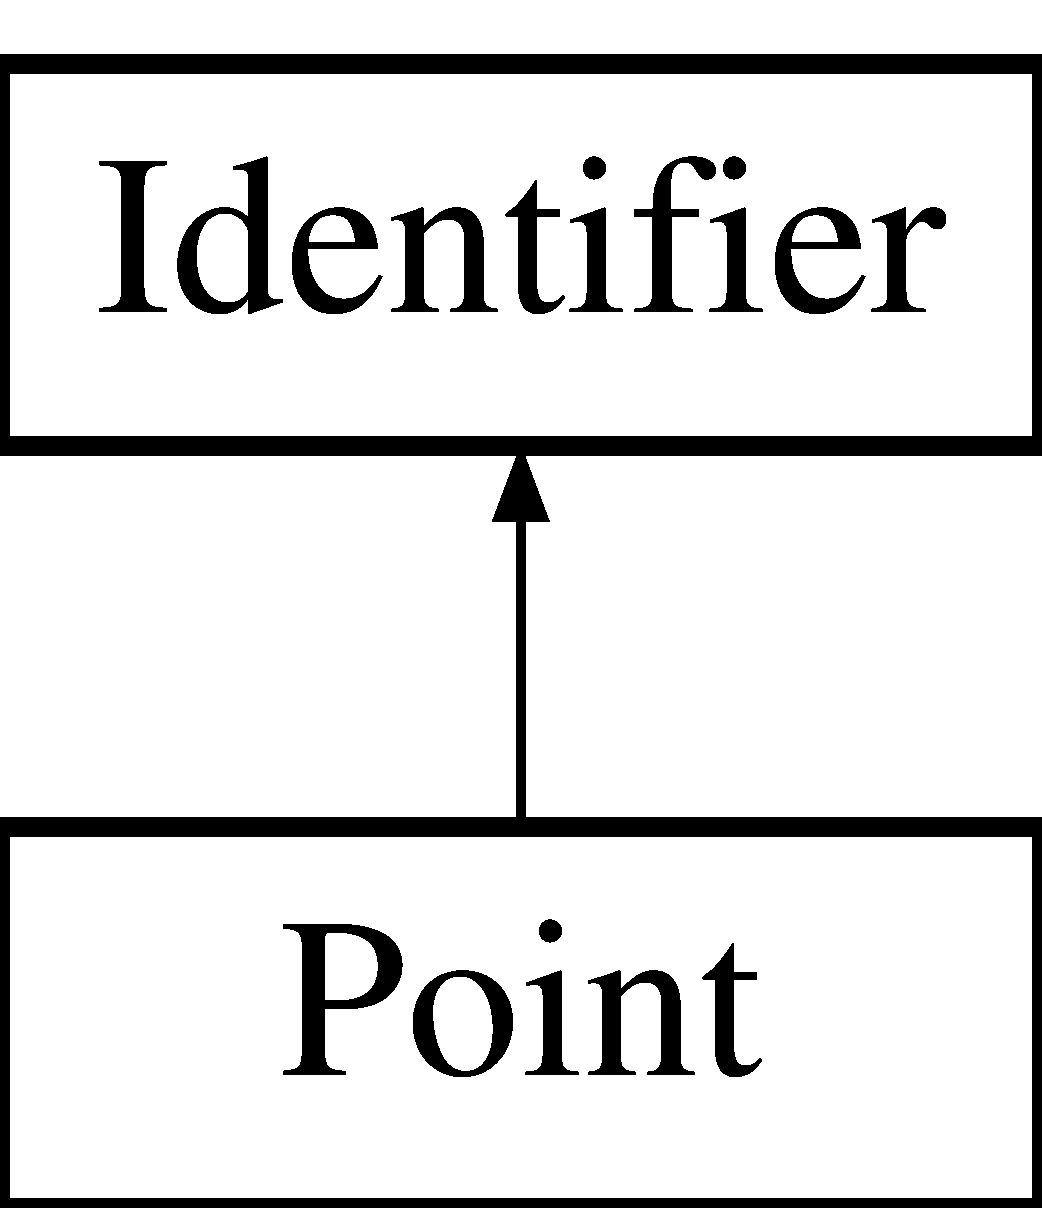
\includegraphics[height=2cm]{classPoint}
\end{center}
\end{figure}
\subsection*{Public Member Functions}
\begin{DoxyCompactItemize}
\item 
\hyperlink{classPoint_a034584b85d239bdd5bd38ab80ab9aee6}{Point} (Real x, Real y)
\item 
\hyperlink{classPoint_ae0b5d58f061678fef344fffa0160ddc3}{Point} (std::vector$<$ Real $>$ const \&coord)
\item 
\hyperlink{classPoint_ac78e6a41f2d39366526d0bc0f1203efd}{Point} (Id id, BcId bcId, Real x, Real y)
\item 
\hypertarget{classPoint_a9717f7833e597160d616b0b643225c37}{
void \hyperlink{classPoint_a9717f7833e597160d616b0b643225c37}{print} (std::ostream \&out) const }
\label{classPoint_a9717f7833e597160d616b0b643225c37}

\begin{DoxyCompactList}\small\item\em print general information about the point \item\end{DoxyCompactList}\item 
\hypertarget{classPoint_a781ea96ab6bb588f2583bbaa5aefea6b}{
Real \hyperlink{classPoint_a781ea96ab6bb588f2583bbaa5aefea6b}{operator\mbox{[}$\,$\mbox{]}} (UInt i) const }
\label{classPoint_a781ea96ab6bb588f2583bbaa5aefea6b}

\begin{DoxyCompactList}\small\item\em return the i-\/th coordinate value \item\end{DoxyCompactList}\end{DoxyCompactItemize}
\subsection*{Static Public Member Functions}
\begin{DoxyCompactItemize}
\item 
\hypertarget{classPoint_aff2972e71baa58292b080fb164de8ca6}{
static constexpr int \hyperlink{classPoint_aff2972e71baa58292b080fb164de8ca6}{dp} ()}
\label{classPoint_aff2972e71baa58292b080fb164de8ca6}

\begin{DoxyCompactList}\small\item\em Returns the number of physical space dimension. \item\end{DoxyCompactList}\item 
\hypertarget{classPoint_a3e43ae96cdd00fe2e6ba73e42031ad55}{
static constexpr int \hyperlink{classPoint_a3e43ae96cdd00fe2e6ba73e42031ad55}{dt} ()}
\label{classPoint_a3e43ae96cdd00fe2e6ba73e42031ad55}

\begin{DoxyCompactList}\small\item\em Returns the number of dimensions used for the search (equal to physical space dimension). \item\end{DoxyCompactList}\item 
\hypertarget{classPoint_a2798999b4a017d89616eb4f5a95ac12b}{
static constexpr int \hyperlink{classPoint_a2798999b4a017d89616eb4f5a95ac12b}{coordsize} ()}
\label{classPoint_a2798999b4a017d89616eb4f5a95ac12b}

\begin{DoxyCompactList}\small\item\em Returns the size of coordinate array. \item\end{DoxyCompactList}\end{DoxyCompactItemize}
\subsection*{Static Public Attributes}
\begin{DoxyCompactItemize}
\item 
static const UInt \hyperlink{classPoint_ac784604377be8075032dcc79d14d7e8b}{ndim} = 2
\end{DoxyCompactItemize}


\subsection{Detailed Description}
This class implements a 2D point. 

\subsection{Constructor \& Destructor Documentation}
\hypertarget{classPoint_a034584b85d239bdd5bd38ab80ab9aee6}{
\index{Point@{Point}!Point@{Point}}
\index{Point@{Point}!Point@{Point}}
\subsubsection[{Point}]{\setlength{\rightskip}{0pt plus 5cm}Point::Point (Real {\em x}, \/  Real {\em y})\hspace{0.3cm}{\ttfamily  \mbox{[}inline\mbox{]}}}}
\label{classPoint_a034584b85d239bdd5bd38ab80ab9aee6}
Another constructor.


\begin{DoxyParams}{Parameters}
\item[\mbox{$\leftarrow$} {\em two}]real, the first is the x-\/coordinate and the second the y-\/coordinate the identifier is set to NVAL \end{DoxyParams}
\hypertarget{classPoint_ae0b5d58f061678fef344fffa0160ddc3}{
\index{Point@{Point}!Point@{Point}}
\index{Point@{Point}!Point@{Point}}
\subsubsection[{Point}]{\setlength{\rightskip}{0pt plus 5cm}Point::Point (std::vector$<$ Real $>$ const \& {\em coord})\hspace{0.3cm}{\ttfamily  \mbox{[}inline\mbox{]}}}}
\label{classPoint_ae0b5d58f061678fef344fffa0160ddc3}
Another constructor.


\begin{DoxyParams}{Parameters}
\item[\mbox{$\leftarrow$} {\em std::vector$<$Real$>$}]it is necessary for the communication with \hyperlink{classADTree}{ADTree} structure the identifier is set to NVAL \end{DoxyParams}
\hypertarget{classPoint_ac78e6a41f2d39366526d0bc0f1203efd}{
\index{Point@{Point}!Point@{Point}}
\index{Point@{Point}!Point@{Point}}
\subsubsection[{Point}]{\setlength{\rightskip}{0pt plus 5cm}Point::Point (Id {\em id}, \/  BcId {\em bcId}, \/  Real {\em x}, \/  Real {\em y})\hspace{0.3cm}{\ttfamily  \mbox{[}inline\mbox{]}}}}
\label{classPoint_ac78e6a41f2d39366526d0bc0f1203efd}
Another constructor.


\begin{DoxyParams}{Parameters}
\item[\mbox{$\leftarrow$} {\em four}]real, the first two are the value for identifier, the other are the x-\/coordinate and the y-\/coordinate \end{DoxyParams}


\subsection{Member Data Documentation}
\hypertarget{classPoint_ac784604377be8075032dcc79d14d7e8b}{
\index{Point@{Point}!ndim@{ndim}}
\index{ndim@{ndim}!Point@{Point}}
\subsubsection[{ndim}]{\setlength{\rightskip}{0pt plus 5cm}const UInt {\bf Point::ndim} = 2\hspace{0.3cm}{\ttfamily  \mbox{[}static\mbox{]}}}}
\label{classPoint_ac784604377be8075032dcc79d14d7e8b}
physical dimension of the point 

The documentation for this class was generated from the following files:\begin{DoxyCompactItemize}
\item 
src/mesh\_\-objects.hpp\item 
src/mesh\_\-objects.cpp\end{DoxyCompactItemize}

\hypertarget{structsplaynode}{
\section{splaynode Struct Reference}
\label{structsplaynode}\index{splaynode@{splaynode}}
}
\subsection*{Public Attributes}
\begin{DoxyCompactItemize}
\item 
\hypertarget{structsplaynode_aaa9fc6e2d568c0be2a5a4c0831965c4f}{
struct \hyperlink{structotri}{otri} {\bfseries keyedge}}
\label{structsplaynode_aaa9fc6e2d568c0be2a5a4c0831965c4f}

\item 
\hypertarget{structsplaynode_a63438aac02b8993141ebf848c347098d}{
vertex {\bfseries keydest}}
\label{structsplaynode_a63438aac02b8993141ebf848c347098d}

\item 
\hypertarget{structsplaynode_a67b52cb89e958acbdf9761ea4aab6813}{
struct \hyperlink{structsplaynode}{splaynode} $\ast$ {\bfseries lchild}}
\label{structsplaynode_a67b52cb89e958acbdf9761ea4aab6813}

\item 
\hypertarget{structsplaynode_ac1cf5f799931eda1315037dc7d0bce3a}{
struct \hyperlink{structsplaynode}{splaynode} $\ast$ {\bfseries rchild}}
\label{structsplaynode_ac1cf5f799931eda1315037dc7d0bce3a}

\end{DoxyCompactItemize}


The documentation for this struct was generated from the following file:\begin{DoxyCompactItemize}
\item 
src/triangle.c\end{DoxyCompactItemize}

\hypertarget{classTree__Header}{
\section{Tree\_\-Header$<$ T $>$ Class Template Reference}
\label{classTree__Header}\index{Tree\_\-Header@{Tree\_\-Header}}
}
\subsection*{Public Member Functions}
\begin{DoxyCompactItemize}
\item 
\hyperlink{classTree__Header_afd804e3208294dabc6f24f597133ec29}{Tree\_\-Header} ()
\item 
\hypertarget{classTree__Header_ac06076ecec5f61bc44066cf5c4008921}{
int \hyperlink{classTree__Header_ac06076ecec5f61bc44066cf5c4008921}{gettreeloc} () const }
\label{classTree__Header_ac06076ecec5f61bc44066cf5c4008921}

\begin{DoxyCompactList}\small\item\em Gets the number of tree memory locations. \item\end{DoxyCompactList}\item 
\hypertarget{classTree__Header_a7bd256dd1c10ba6c8ef064f133695a8b}{
void \hyperlink{classTree__Header_a7bd256dd1c10ba6c8ef064f133695a8b}{settreeloc} (int const \&nt)}
\label{classTree__Header_a7bd256dd1c10ba6c8ef064f133695a8b}

\begin{DoxyCompactList}\small\item\em Sets the number of tree memory locations (handles a \hyperlink{classLocLengthError}{LocLengthError} exception). \item\end{DoxyCompactList}\item 
\hypertarget{classTree__Header_a8fd3e3d0451690385b00417f841f06e4}{
int \hyperlink{classTree__Header_a8fd3e3d0451690385b00417f841f06e4}{gettreelev} () const }
\label{classTree__Header_a8fd3e3d0451690385b00417f841f06e4}

\begin{DoxyCompactList}\small\item\em Gets the number of tree levels. \item\end{DoxyCompactList}\item 
\hypertarget{classTree__Header_a4144fe52a6ddf6f4db7b3084e8d3f881}{
void \hyperlink{classTree__Header_a4144fe52a6ddf6f4db7b3084e8d3f881}{settreelev} (int const \&nl)}
\label{classTree__Header_a4144fe52a6ddf6f4db7b3084e8d3f881}

\begin{DoxyCompactList}\small\item\em Sets the number of tree levels. \item\end{DoxyCompactList}\item 
\hypertarget{classTree__Header_a7f2d1853d95363ac137b9f942a81a318}{
int \hyperlink{classTree__Header_a7f2d1853d95363ac137b9f942a81a318}{getndimp} () const }
\label{classTree__Header_a7f2d1853d95363ac137b9f942a81a318}

\begin{DoxyCompactList}\small\item\em Gets the number of physical space dimension. \item\end{DoxyCompactList}\item 
\hypertarget{classTree__Header_ad5ee863231e81dc6d388bc183c5b35f1}{
int \hyperlink{classTree__Header_ad5ee863231e81dc6d388bc183c5b35f1}{getnkey} () const }
\label{classTree__Header_ad5ee863231e81dc6d388bc183c5b35f1}

\begin{DoxyCompactList}\small\item\em Gets the number of pieces of information carried by the tree. \item\end{DoxyCompactList}\item 
\hypertarget{classTree__Header_a5a6166156d8b01a0847cebab161eab59}{
int \hyperlink{classTree__Header_a5a6166156d8b01a0847cebab161eab59}{getndimt} () const }
\label{classTree__Header_a5a6166156d8b01a0847cebab161eab59}

\begin{DoxyCompactList}\small\item\em Gets the number of dimensions used for the search. \item\end{DoxyCompactList}\item 
\hypertarget{classTree__Header_a2c3816734f8e1269250d4c68fe7acf46}{
int \hyperlink{classTree__Header_a2c3816734f8e1269250d4c68fe7acf46}{getnele} () const }
\label{classTree__Header_a2c3816734f8e1269250d4c68fe7acf46}

\begin{DoxyCompactList}\small\item\em Gets the number of logical locations currently used in the tree. \item\end{DoxyCompactList}\item 
\hypertarget{classTree__Header_ad403a6445724b73435247700a2204a7c}{
void \hyperlink{classTree__Header_ad403a6445724b73435247700a2204a7c}{setnele} (int const \&ne)}
\label{classTree__Header_ad403a6445724b73435247700a2204a7c}

\begin{DoxyCompactList}\small\item\em Sets the number of logical locations currently used in the tree. \item\end{DoxyCompactList}\item 
\hypertarget{classTree__Header_a004054503f011bbbdaae66160533eec0}{
int \hyperlink{classTree__Header_a004054503f011bbbdaae66160533eec0}{getiava} () const }
\label{classTree__Header_a004054503f011bbbdaae66160533eec0}

\begin{DoxyCompactList}\small\item\em Gets the next available location in the stack. \item\end{DoxyCompactList}\item 
\hypertarget{classTree__Header_a60dc5cf68125321d1430caa41a7c81eb}{
void \hyperlink{classTree__Header_a60dc5cf68125321d1430caa41a7c81eb}{setiava} (int const \&ia)}
\label{classTree__Header_a60dc5cf68125321d1430caa41a7c81eb}

\begin{DoxyCompactList}\small\item\em Sets the next available location in the stack. \item\end{DoxyCompactList}\item 
\hypertarget{classTree__Header_a37fc3f03126c6df299bef979d1683d4a}{
int \hyperlink{classTree__Header_a37fc3f03126c6df299bef979d1683d4a}{getiend} () const }
\label{classTree__Header_a37fc3f03126c6df299bef979d1683d4a}

\begin{DoxyCompactList}\small\item\em Gets the next available location in the tree free store. \item\end{DoxyCompactList}\item 
\hypertarget{classTree__Header_a915e46ea6d11fad48babb4364cb3af9b}{
void \hyperlink{classTree__Header_a915e46ea6d11fad48babb4364cb3af9b}{setiend} (int const \&ie)}
\label{classTree__Header_a915e46ea6d11fad48babb4364cb3af9b}

\begin{DoxyCompactList}\small\item\em Sets the next available location in the tree free store. \item\end{DoxyCompactList}\item 
\hypertarget{classTree__Header_af9ca5ec4f523ecb763b794981d81ea3d}{
double \hyperlink{classTree__Header_af9ca5ec4f523ecb763b794981d81ea3d}{domainorig} (int const \&i) const }
\label{classTree__Header_af9ca5ec4f523ecb763b794981d81ea3d}

\begin{DoxyCompactList}\small\item\em Gets the i-\/th coordinate of the origin of the tree's (domain) bounding box. -\/-\/$>$ queste falle friend. \item\end{DoxyCompactList}\item 
\hypertarget{classTree__Header_aa9e681ec8d883f09ba7ff72b2455dfbf}{
double \hyperlink{classTree__Header_aa9e681ec8d883f09ba7ff72b2455dfbf}{domainscal} (int const \&i) const }
\label{classTree__Header_aa9e681ec8d883f09ba7ff72b2455dfbf}

\begin{DoxyCompactList}\small\item\em Gets the i-\/th scaling factor of the tree's bounding box. \item\end{DoxyCompactList}\end{DoxyCompactItemize}
\subsection*{Protected Member Functions}
\begin{DoxyCompactItemize}
\item 
\hyperlink{classTree__Header_a49b84b2440c27da71ae944cb94d8d856}{Tree\_\-Header} (int const \&ntree, int const \&nk, \hyperlink{classDomain}{Domain}$<$ T $>$ const \&d)
\item 
\hypertarget{classTree__Header_a104a3f95557ea8f3152737e1af13fa6c}{
void \hyperlink{classTree__Header_a104a3f95557ea8f3152737e1af13fa6c}{stml} (int const \&nt)}
\label{classTree__Header_a104a3f95557ea8f3152737e1af13fa6c}

\begin{DoxyCompactList}\small\item\em Tries to set the number of tree memory locations (throws a \hyperlink{classLocLengthError}{LocLengthError} exception if nt is out of range). \item\end{DoxyCompactList}\end{DoxyCompactItemize}
\subsection*{Protected Attributes}
\begin{DoxyCompactItemize}
\item 
\hypertarget{classTree__Header_aa165ee770e4080623c7d5f0bbb26e112}{
int \hyperlink{classTree__Header_aa165ee770e4080623c7d5f0bbb26e112}{tree\_\-loc\_\-}}
\label{classTree__Header_aa165ee770e4080623c7d5f0bbb26e112}

\begin{DoxyCompactList}\small\item\em Tree memory locations. \item\end{DoxyCompactList}\item 
\hypertarget{classTree__Header_ae34b890a2ee5dc2db4993e7a1f030742}{
int \hyperlink{classTree__Header_ae34b890a2ee5dc2db4993e7a1f030742}{tree\_\-lev\_\-}}
\label{classTree__Header_ae34b890a2ee5dc2db4993e7a1f030742}

\begin{DoxyCompactList}\small\item\em Tree levels. \item\end{DoxyCompactList}\item 
\hypertarget{classTree__Header_a7a8cfae962f92cf73e86946235f649d2}{
int \hyperlink{classTree__Header_a7a8cfae962f92cf73e86946235f649d2}{ndimp\_\-}}
\label{classTree__Header_a7a8cfae962f92cf73e86946235f649d2}

\begin{DoxyCompactList}\small\item\em Number of physical space dimensions (typically 2 or 3). \item\end{DoxyCompactList}\item 
\hypertarget{classTree__Header_a1759b541ad1f2c1d4af7628c64085eb1}{
int \hyperlink{classTree__Header_a1759b541ad1f2c1d4af7628c64085eb1}{nkey\_\-}}
\label{classTree__Header_a1759b541ad1f2c1d4af7628c64085eb1}

\begin{DoxyCompactList}\small\item\em Number of pieces of information carried by the tree. The size of each node is nkey+2 words. \item\end{DoxyCompactList}\item 
\hypertarget{classTree__Header_a9a2b7a443a6fefb534b6b77ba6d1e204}{
int \hyperlink{classTree__Header_a9a2b7a443a6fefb534b6b77ba6d1e204}{ndimt\_\-}}
\label{classTree__Header_a9a2b7a443a6fefb534b6b77ba6d1e204}

\begin{DoxyCompactList}\small\item\em Number of dimensions used for the search (2$\ast$ndimp because we use box). \item\end{DoxyCompactList}\item 
\hypertarget{classTree__Header_ace612fcc68b5566feff81a8e854ab1aa}{
int \hyperlink{classTree__Header_ace612fcc68b5566feff81a8e854ab1aa}{nele\_\-}}
\label{classTree__Header_ace612fcc68b5566feff81a8e854ab1aa}

\begin{DoxyCompactList}\small\item\em Number of logical locations currently used in the tree. Initialized to 0. \item\end{DoxyCompactList}\item 
\hypertarget{classTree__Header_a5ef170aea71ef926da23bcd55ede4129}{
\hyperlink{classDomain}{Domain}$<$ T $>$ \hyperlink{classTree__Header_a5ef170aea71ef926da23bcd55ede4129}{tree\_\-domain\_\-}}
\label{classTree__Header_a5ef170aea71ef926da23bcd55ede4129}

\begin{DoxyCompactList}\small\item\em Tree's domain. \item\end{DoxyCompactList}\end{DoxyCompactItemize}
\begin{Indent}{\bf Tree indices}\par
{\em \label{_amgrpca0f741e429d5e561c4e48b1890518fc}
 The use of iava and iend avoids the necessity of initializing the stack of available locations. In fact, the stack contains only locations that have been previously deleted from the tree. }\begin{DoxyCompactItemize}
\item 
int \hyperlink{classTree__Header_a106cee8ef2a9bc2b15a2ea97bc11d72b}{iava\_\-}
\item 
int \hyperlink{classTree__Header_a9f4dfb8c0a7077d7c465202d1c9c6a21}{iend\_\-}
\end{DoxyCompactItemize}
\end{Indent}
\subsection*{Friends}
\begin{DoxyCompactItemize}
\item 
{\footnotesize template$<$class S $>$ }\\std::ostream \& \hyperlink{classTree__Header_a444b2368a05d862bc11bf418e11c5e51}{operator$<$$<$} (std::ostream \&, \hyperlink{classTree__Header}{Tree\_\-Header}$<$ S $>$ const \&)
\item 
{\footnotesize template$<$class S $>$ }\\\hyperlink{classTree__Header}{Tree\_\-Header}$<$ S $>$ \hyperlink{classTree__Header_a0b108322f91afa71aae8698e1da6cda8}{createtreeheader} (int const \&nt, int const \&nk, \hyperlink{classDomain}{Domain}$<$ S $>$ const \&d)
\begin{DoxyCompactList}\small\item\em Creates a tree header handling the exception condition in which tree maximum dimension is exceeded. \item\end{DoxyCompactList}\end{DoxyCompactItemize}
\subsubsection*{template$<$class T$>$ class Tree\_\-Header$<$ T $>$}



\subsection{Constructor \& Destructor Documentation}
\hypertarget{classTree__Header_a49b84b2440c27da71ae944cb94d8d856}{
\index{Tree\_\-Header@{Tree\_\-Header}!Tree\_\-Header@{Tree\_\-Header}}
\index{Tree\_\-Header@{Tree\_\-Header}!Tree_Header@{Tree\_\-Header}}
\subsubsection[{Tree\_\-Header}]{\setlength{\rightskip}{0pt plus 5cm}template$<$class T$>$ {\bf Tree\_\-Header}$<$ T $>$::{\bf Tree\_\-Header} (int const \& {\em ntree}, \/  int const \& {\em nk}, \/  {\bf Domain}$<$ T $>$ const \& {\em d})\hspace{0.3cm}{\ttfamily  \mbox{[}inline, protected\mbox{]}}}}
\label{classTree__Header_a49b84b2440c27da71ae944cb94d8d856}
A protected constructor.


\begin{DoxyParams}{Parameters}
\item[\mbox{$\leftarrow$} {\em ntree}]Tree dimension needed. \item[\mbox{$\leftarrow$} {\em nk}]Number of pieces of information carried by the tree. \item[\mbox{$\leftarrow$} {\em d}]Tree's domain.\end{DoxyParams}
Public function createtreeheader must be used to create an object of \hyperlink{classHeader}{Header} class. This avoids the creation of a tree with more memory locations than a fixed limit. \hypertarget{classTree__Header_afd804e3208294dabc6f24f597133ec29}{
\index{Tree\_\-Header@{Tree\_\-Header}!Tree\_\-Header@{Tree\_\-Header}}
\index{Tree\_\-Header@{Tree\_\-Header}!Tree_Header@{Tree\_\-Header}}
\subsubsection[{Tree\_\-Header}]{\setlength{\rightskip}{0pt plus 5cm}template$<$class T$>$ {\bf Tree\_\-Header}$<$ T $>$::{\bf Tree\_\-Header} ()\hspace{0.3cm}{\ttfamily  \mbox{[}inline\mbox{]}}}}
\label{classTree__Header_afd804e3208294dabc6f24f597133ec29}
Default constructor.

It's fundamental in creating an \hyperlink{classADTree}{ADTree} object from a MeshFile::ff2dmesh or a MeshFile::ff3dmesh object. 

\subsection{Friends And Related Function Documentation}
\hypertarget{classTree__Header_a0b108322f91afa71aae8698e1da6cda8}{
\index{Tree\_\-Header@{Tree\_\-Header}!createtreeheader@{createtreeheader}}
\index{createtreeheader@{createtreeheader}!Tree_Header@{Tree\_\-Header}}
\subsubsection[{createtreeheader}]{\setlength{\rightskip}{0pt plus 5cm}template$<$class T$>$ template$<$class S $>$ {\bf Header}$<$ S $>$ {\bf Tree\_\-Header}$<$ T $>$::createtreeheader (int const \& {\em nt}, \/  int const \& {\em nk}, \/  {\bf Domain}$<$ S $>$ const \& {\em d})\hspace{0.3cm}{\ttfamily  \mbox{[}friend\mbox{]}}}}
\label{classTree__Header_a0b108322f91afa71aae8698e1da6cda8}


Creates a tree header handling the exception condition in which tree maximum dimension is exceeded. 
\begin{DoxyParams}{Parameters}
\item[\mbox{$\leftarrow$} {\em nt}]Tree dimension needed. \item[\mbox{$\leftarrow$} {\em nk}]Number of pieces of information carried by the tree. \item[\mbox{$\leftarrow$} {\em d}]Tree's domain. \end{DoxyParams}
\hypertarget{classTree__Header_a444b2368a05d862bc11bf418e11c5e51}{
\index{Tree\_\-Header@{Tree\_\-Header}!operator$<$$<$@{operator$<$$<$}}
\index{operator$<$$<$@{operator$<$$<$}!Tree_Header@{Tree\_\-Header}}
\subsubsection[{operator$<$$<$}]{\setlength{\rightskip}{0pt plus 5cm}template$<$class T$>$ template$<$class S $>$ std::ostream\& operator$<$$<$ (std::ostream \&, \/  {\bf Tree\_\-Header}$<$ S $>$ const \&)\hspace{0.3cm}{\ttfamily  \mbox{[}friend\mbox{]}}}}
\label{classTree__Header_a444b2368a05d862bc11bf418e11c5e51}
Output operator.

It prints out:
\begin{DoxyItemize}
\item number of tree memory locations;
\item number of tree levels;
\item number of physical space dimensions;
\item number of pieces of information carried by the tree;
\item number of dimensions used for the search;
\item number of logical locations currently used in the tree;
\item tree domain. 
\end{DoxyItemize}

\subsection{Member Data Documentation}
\hypertarget{classTree__Header_a106cee8ef2a9bc2b15a2ea97bc11d72b}{
\index{Tree\_\-Header@{Tree\_\-Header}!iava\_\-@{iava\_\-}}
\index{iava\_\-@{iava\_\-}!Tree_Header@{Tree\_\-Header}}
\subsubsection[{iava\_\-}]{\setlength{\rightskip}{0pt plus 5cm}template$<$class T$>$ int {\bf Tree\_\-Header}$<$ T $>$::{\bf iava\_\-}\hspace{0.3cm}{\ttfamily  \mbox{[}protected\mbox{]}}}}
\label{classTree__Header_a106cee8ef2a9bc2b15a2ea97bc11d72b}
Next available location in the stack. Initialized to 1.

The stack of available nodes is a linked list with all nodes that have been previously deleted. If iava=0 the stack is empty. \hypertarget{classTree__Header_a9f4dfb8c0a7077d7c465202d1c9c6a21}{
\index{Tree\_\-Header@{Tree\_\-Header}!iend\_\-@{iend\_\-}}
\index{iend\_\-@{iend\_\-}!Tree_Header@{Tree\_\-Header}}
\subsubsection[{iend\_\-}]{\setlength{\rightskip}{0pt plus 5cm}template$<$class T$>$ int {\bf Tree\_\-Header}$<$ T $>$::{\bf iend\_\-}\hspace{0.3cm}{\ttfamily  \mbox{[}protected\mbox{]}}}}
\label{classTree__Header_a9f4dfb8c0a7077d7c465202d1c9c6a21}
Next available location in the yet not allocated part of the tree (\char`\"{}tree free store\char`\"{}). Initialized to 1.

The \char`\"{}tree free store\char`\"{} is the yet unassigned portion of the vector storing the tree. It effectively acts as a free storage area. If iend=1, the free storage is at his maximum size. iend never decreases. It may increase during insertions and will always remain unaltered after deletions. It isn't equal to nele. 

The documentation for this class was generated from the following files:\begin{DoxyCompactItemize}
\item 
src/\hyperlink{tree__header_8hpp}{tree\_\-header.hpp}\item 
src/tree\_\-header\_\-imp.hpp\end{DoxyCompactItemize}

\hypertarget{classTreeAlloc}{
\section{TreeAlloc$<$ Shape $>$ Class Template Reference}
\label{classTreeAlloc}\index{TreeAlloc@{TreeAlloc}}
}


{\ttfamily \#include $<$exception\_\-handling.hpp$>$}Inheritance diagram for TreeAlloc$<$ Shape $>$::\begin{figure}[H]
\begin{center}
\leavevmode
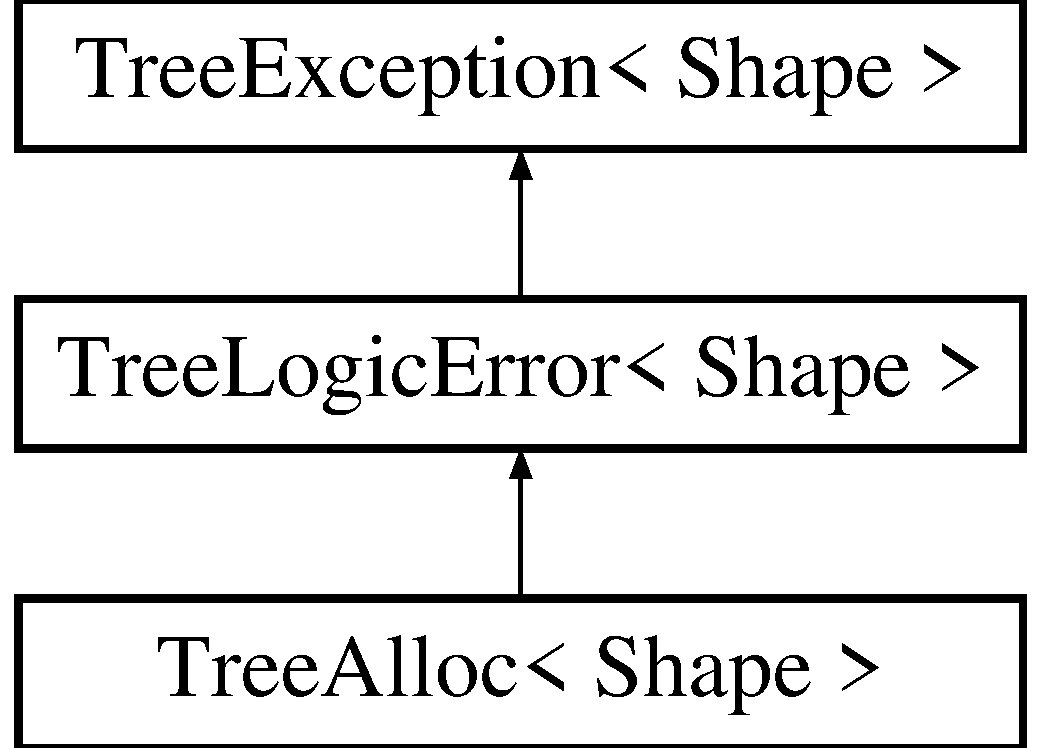
\includegraphics[height=3cm]{classTreeAlloc}
\end{center}
\end{figure}


\subsection{Detailed Description}
\subsubsection*{template$<$class Shape$>$ class TreeAlloc$<$ Shape $>$}

This class is used to report the exception condition in which there is no more space in the tree to store a new node. 

The documentation for this class was generated from the following file:\begin{DoxyCompactItemize}
\item 
src/\hyperlink{exception__handling_8hpp}{exception\_\-handling.hpp}\end{DoxyCompactItemize}

\hypertarget{classTreeDomainError}{
\section{TreeDomainError$<$ Shape $>$ Class Template Reference}
\label{classTreeDomainError}\index{TreeDomainError@{TreeDomainError}}
}


{\ttfamily \#include $<$exception\_\-handling.hpp$>$}Inheritance diagram for TreeDomainError$<$ Shape $>$::\begin{figure}[H]
\begin{center}
\leavevmode
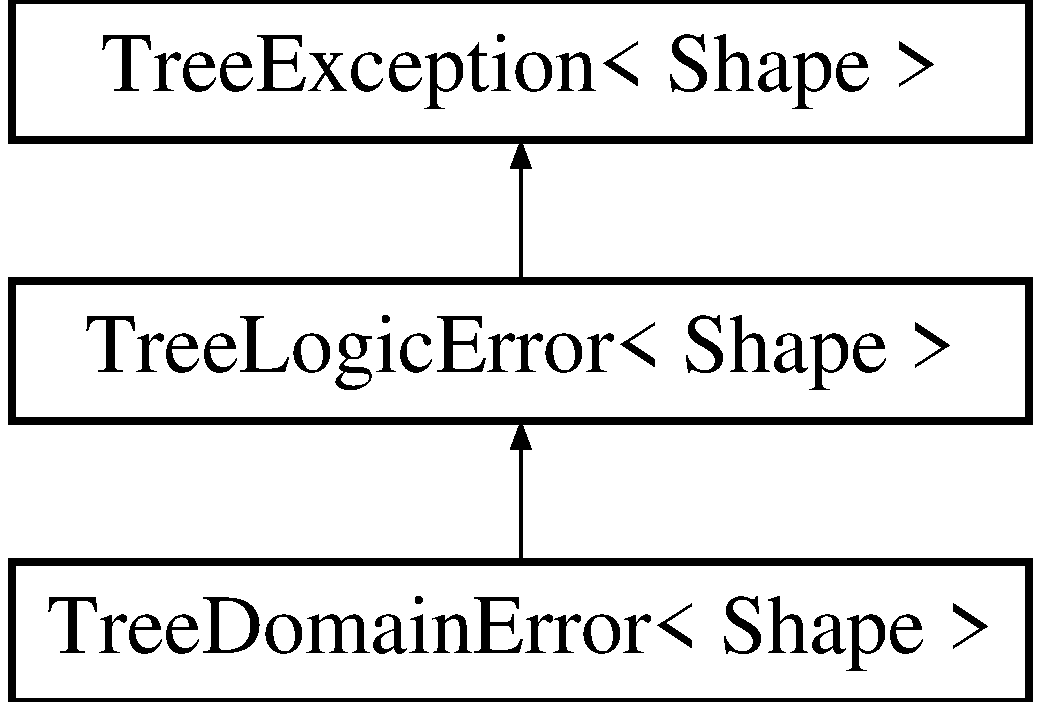
\includegraphics[height=3cm]{classTreeDomainError}
\end{center}
\end{figure}
\subsection*{Public Member Functions}
\begin{DoxyCompactItemize}
\item 
\hyperlink{classTreeDomainError_a36c6d072485354991aa96f295f545f2c}{TreeDomainError} (int const \&np1, int const \&size, std::vector$<$ Real $>$ const coord)
\item 
\hypertarget{classTreeDomainError_a5f366c57baa089fed8fd70dd1039c9a8}{
int \hyperlink{classTreeDomainError_a5f366c57baa089fed8fd70dd1039c9a8}{getnelep1} () const }
\label{classTreeDomainError_a5f366c57baa089fed8fd70dd1039c9a8}

\begin{DoxyCompactList}\small\item\em Returns number of logical locations currently used in the tree plus 1. \item\end{DoxyCompactList}\end{DoxyCompactItemize}
\subsection*{Protected Attributes}
\begin{DoxyCompactItemize}
\item 
\hypertarget{classTreeDomainError_ab6f1f38f2cff2ee9c561e49ec678069d}{
int \hyperlink{classTreeDomainError_ab6f1f38f2cff2ee9c561e49ec678069d}{nelep1}}
\label{classTreeDomainError_ab6f1f38f2cff2ee9c561e49ec678069d}

\begin{DoxyCompactList}\small\item\em Number of logical locations currently used in the tree plus 1. \item\end{DoxyCompactList}\item 
\hypertarget{classTreeDomainError_a4549e1a6439fcfc9a581505e21f3fcec}{
int \hyperlink{classTreeDomainError_a4549e1a6439fcfc9a581505e21f3fcec}{csize}}
\label{classTreeDomainError_a4549e1a6439fcfc9a581505e21f3fcec}

\begin{DoxyCompactList}\small\item\em Size of the array storing the coordinates of the object which is out of domain. \item\end{DoxyCompactList}\item 
\hypertarget{classTreeDomainError_a181c509a5e1dbcf4c3b2f0c1918a8345}{
std::vector$<$ Real $>$ \hyperlink{classTreeDomainError_a181c509a5e1dbcf4c3b2f0c1918a8345}{outobj}}
\label{classTreeDomainError_a181c509a5e1dbcf4c3b2f0c1918a8345}

\begin{DoxyCompactList}\small\item\em Coordinates of the object which is out of domain. \item\end{DoxyCompactList}\end{DoxyCompactItemize}
\subsection*{Friends}
\begin{DoxyCompactItemize}
\item 
{\footnotesize template$<$class T $>$ }\\std::ostream \& \hyperlink{classTreeDomainError_a25d8eeca1719586bbbaeac6a01aa178b}{operator$<$$<$} (std::ostream \&ostr, \hyperlink{classTreeDomainError}{TreeDomainError}$<$ T $>$ const \&de)
\end{DoxyCompactItemize}


\subsection{Detailed Description}
\subsubsection*{template$<$class Shape$>$ class TreeDomainError$<$ Shape $>$}

This class is used to report the exception condition in which an object is out of domain. 

\subsection{Constructor \& Destructor Documentation}
\hypertarget{classTreeDomainError_a36c6d072485354991aa96f295f545f2c}{
\index{TreeDomainError@{TreeDomainError}!TreeDomainError@{TreeDomainError}}
\index{TreeDomainError@{TreeDomainError}!TreeDomainError@{TreeDomainError}}
\subsubsection[{TreeDomainError}]{\setlength{\rightskip}{0pt plus 5cm}template$<$class Shape $>$ {\bf TreeDomainError}$<$ Shape $>$::{\bf TreeDomainError} (int const \& {\em np1}, \/  int const \& {\em size}, \/  std::vector$<$ Real $>$ const  {\em coord})\hspace{0.3cm}{\ttfamily  \mbox{[}inline\mbox{]}}}}
\label{classTreeDomainError_a36c6d072485354991aa96f295f545f2c}
A constructor. 

\subsection{Friends And Related Function Documentation}
\hypertarget{classTreeDomainError_a25d8eeca1719586bbbaeac6a01aa178b}{
\index{TreeDomainError@{TreeDomainError}!operator$<$$<$@{operator$<$$<$}}
\index{operator$<$$<$@{operator$<$$<$}!TreeDomainError@{TreeDomainError}}
\subsubsection[{operator$<$$<$}]{\setlength{\rightskip}{0pt plus 5cm}template$<$class Shape$>$ template$<$class T $>$ std::ostream\& operator$<$$<$ (std::ostream \& {\em ostr}, \/  {\bf TreeDomainError}$<$ T $>$ const \& {\em de})\hspace{0.3cm}{\ttfamily  \mbox{[}friend\mbox{]}}}}
\label{classTreeDomainError_a25d8eeca1719586bbbaeac6a01aa178b}
Output operator.

It outputs coordinates of the object which is out of domain. 

The documentation for this class was generated from the following file:\begin{DoxyCompactItemize}
\item 
src/\hyperlink{exception__handling_8hpp}{exception\_\-handling.hpp}\end{DoxyCompactItemize}

\hypertarget{classTreeException}{
\section{TreeException$<$ Shape $>$ Class Template Reference}
\label{classTreeException}\index{TreeException@{TreeException}}
}


{\ttfamily \#include $<$exception\_\-handling.hpp$>$}Inheritance diagram for TreeException$<$ Shape $>$::\begin{figure}[H]
\begin{center}
\leavevmode
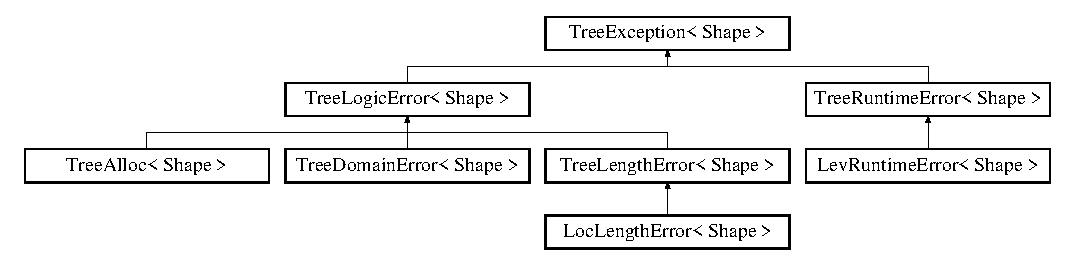
\includegraphics[height=3.11111cm]{classTreeException}
\end{center}
\end{figure}


\subsection{Detailed Description}
\subsubsection*{template$<$class Shape$>$ class TreeException$<$ Shape $>$}

All exceptions thrown from the adtree library are derived from the base class \hyperlink{classTreeException}{TreeException}. 

The documentation for this class was generated from the following file:\begin{DoxyCompactItemize}
\item 
src/\hyperlink{exception__handling_8hpp}{exception\_\-handling.hpp}\end{DoxyCompactItemize}

\hypertarget{classTreeLengthError}{
\section{TreeLengthError$<$ Shape $>$ Class Template Reference}
\label{classTreeLengthError}\index{TreeLengthError@{TreeLengthError}}
}


{\ttfamily \#include $<$exception\_\-handling.hpp$>$}Inheritance diagram for TreeLengthError$<$ Shape $>$::\begin{figure}[H]
\begin{center}
\leavevmode
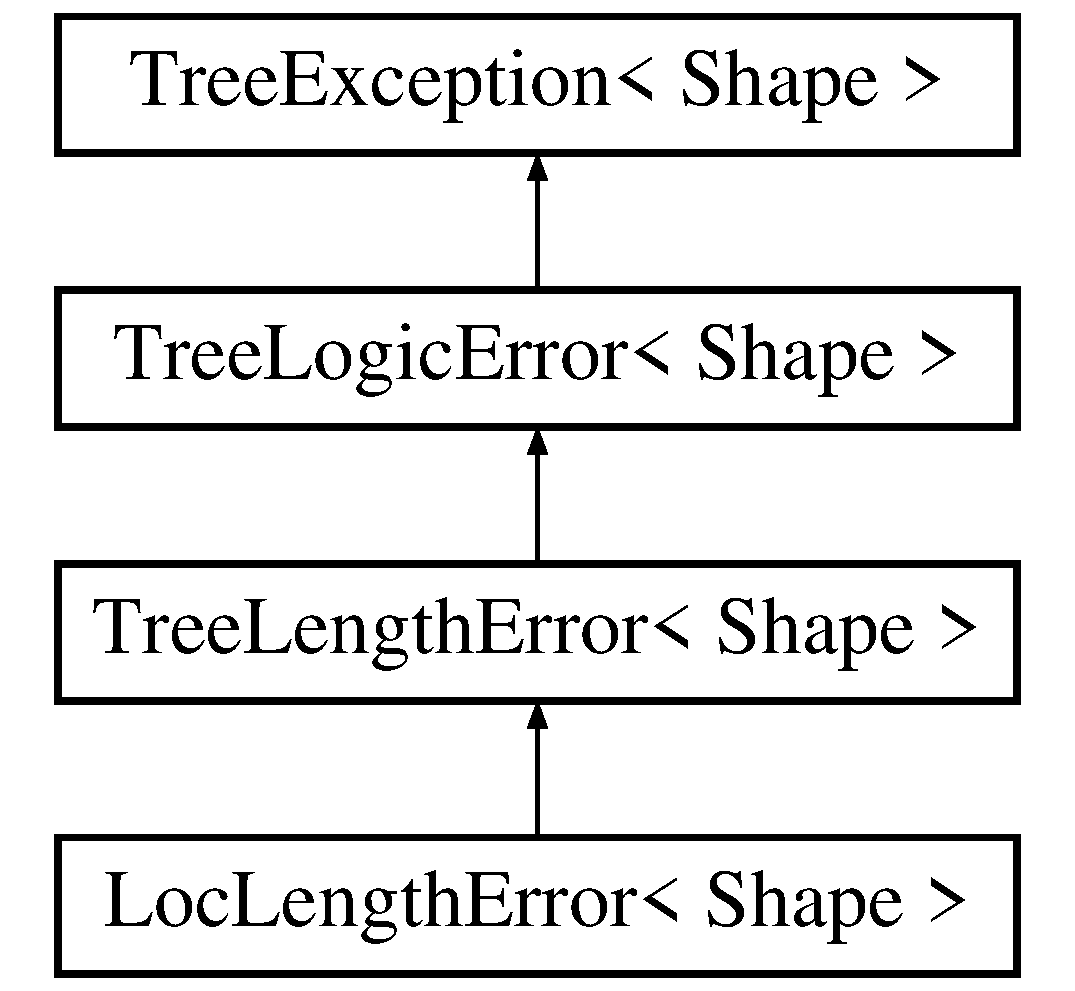
\includegraphics[height=4cm]{classTreeLengthError}
\end{center}
\end{figure}


\subsection{Detailed Description}
\subsubsection*{template$<$class Shape$>$ class TreeLengthError$<$ Shape $>$}

This class is used to report an attempt to do something that exceeds a maximum allowable size concerning the tree. 

The documentation for this class was generated from the following file:\begin{DoxyCompactItemize}
\item 
src/\hyperlink{exception__handling_8hpp}{exception\_\-handling.hpp}\end{DoxyCompactItemize}

\hypertarget{classTreeLogicError}{
\section{TreeLogicError$<$ Shape $>$ Class Template Reference}
\label{classTreeLogicError}\index{TreeLogicError@{TreeLogicError}}
}


{\ttfamily \#include $<$exception\_\-handling.hpp$>$}Inheritance diagram for TreeLogicError$<$ Shape $>$::\begin{figure}[H]
\begin{center}
\leavevmode
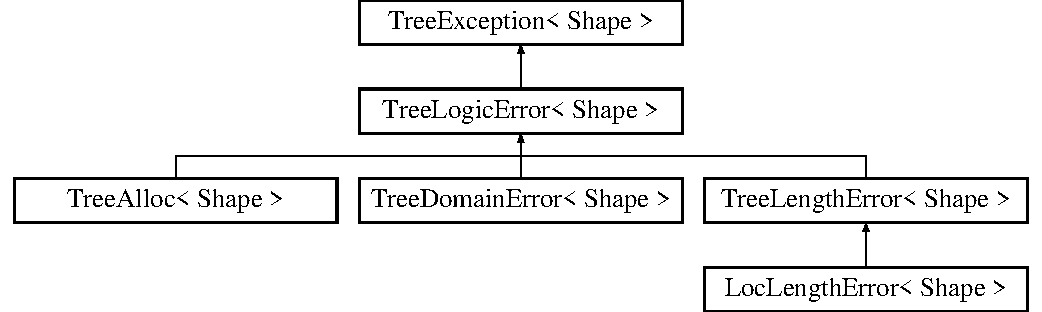
\includegraphics[height=4cm]{classTreeLogicError}
\end{center}
\end{figure}


\subsection{Detailed Description}
\subsubsection*{template$<$class Shape$>$ class TreeLogicError$<$ Shape $>$}

This class is used to report a logic error concerning the tree, i.e. an error that, at least in theory, could be avoided by the program; for example, by performing additional tests of function arguments. 

The documentation for this class was generated from the following file:\begin{DoxyCompactItemize}
\item 
src/\hyperlink{exception__handling_8hpp}{exception\_\-handling.hpp}\end{DoxyCompactItemize}

\hypertarget{classTreeNode}{
\section{TreeNode$<$ Shape $>$ Class Template Reference}
\label{classTreeNode}\index{TreeNode@{TreeNode}}
}


Class defining a tree node.  


{\ttfamily \#include $<$treenode.hpp$>$}\subsection*{Public Member Functions}
\begin{DoxyCompactItemize}
\item 
\hyperlink{classTreeNode_a0b76dda42f063815700904c6861055b2}{TreeNode} ()
\item 
\hyperlink{classTreeNode_a8fc5141645c0a2131e3d4148da085165}{TreeNode} (Id const id, Shape shape, std::vector$<$ int $>$ const \&keys)
\item 
\hypertarget{classTreeNode_a8625cb7bfd1b093017060c0573fd5264}{
void \hyperlink{classTreeNode_a8625cb7bfd1b093017060c0573fd5264}{setfather} (int const \&ifth)}
\label{classTreeNode_a8625cb7bfd1b093017060c0573fd5264}

\begin{DoxyCompactList}\small\item\em Sets the father. \item\end{DoxyCompactList}\item 
void \hyperlink{classTreeNode_a5dc66c89b3e2a3a46600f08f0dad5b80}{setchild} (short int const \&flag, int const \&child)
\begin{DoxyCompactList}\small\item\em Sets a child. \item\end{DoxyCompactList}\item 
\hypertarget{classTreeNode_a687e35a6d01acbc98f0f7ba385548122}{
int \hyperlink{classTreeNode_a687e35a6d01acbc98f0f7ba385548122}{getfather} () const }
\label{classTreeNode_a687e35a6d01acbc98f0f7ba385548122}

\begin{DoxyCompactList}\small\item\em Returns the father. \item\end{DoxyCompactList}\item 
int \hyperlink{classTreeNode_ae48bc7d93db5bbbfb8950cf309e17cb3}{getchild} (short int const \&flag) const 
\begin{DoxyCompactList}\small\item\em Returns a child. \item\end{DoxyCompactList}\item 
\hypertarget{classTreeNode_ad659a94dd818b13ec165033caccedd22}{
void \hyperlink{classTreeNode_ad659a94dd818b13ec165033caccedd22}{setcoords} (std::vector$<$ Real $>$ const \&data)}
\label{classTreeNode_ad659a94dd818b13ec165033caccedd22}

\begin{DoxyCompactList}\small\item\em Sets the coordinates of the bbox stored in the node. \item\end{DoxyCompactList}\item 
\hypertarget{classTreeNode_a3eb758dc2378eae56e2b365bae71e909}{
Real \hyperlink{classTreeNode_a3eb758dc2378eae56e2b365bae71e909}{getcoord} (int const \&i) const }
\label{classTreeNode_a3eb758dc2378eae56e2b365bae71e909}

\begin{DoxyCompactList}\small\item\em Gets the i-\/th coordinate of the bounding box of the object stored in the node. \item\end{DoxyCompactList}\item 
\hypertarget{classTreeNode_a4bdc3e9bd742427b7e5ca3c6db7c3ff6}{
void \hyperlink{classTreeNode_a4bdc3e9bd742427b7e5ca3c6db7c3ff6}{setid} (Id id)}
\label{classTreeNode_a4bdc3e9bd742427b7e5ca3c6db7c3ff6}

\begin{DoxyCompactList}\small\item\em Sets the id stored in the node. \item\end{DoxyCompactList}\item 
\hypertarget{classTreeNode_ae18786d641caa8c97511a05e47405708}{
Id \hyperlink{classTreeNode_ae18786d641caa8c97511a05e47405708}{getid} () const }
\label{classTreeNode_ae18786d641caa8c97511a05e47405708}

\begin{DoxyCompactList}\small\item\em Gets id stored in the node. \item\end{DoxyCompactList}\item 
void \hyperlink{classTreeNode_a18c8b24477006cf279fcb5b08fc8b65d}{setkeys} (std::vector$<$ int $>$ const \&k)
\begin{DoxyCompactList}\small\item\em Gets the i-\/th coordinate value of the p-\/th vertex. \item\end{DoxyCompactList}\item 
\hypertarget{classTreeNode_a06f21fbc6588ad144778d045a4798612}{
std::vector$<$ int $>$ \hyperlink{classTreeNode_a06f21fbc6588ad144778d045a4798612}{getkeys} () const }
\label{classTreeNode_a06f21fbc6588ad144778d045a4798612}

\begin{DoxyCompactList}\small\item\em Gets the additional informations stored in the node. \item\end{DoxyCompactList}\item 
\hypertarget{classTreeNode_a8a3bcea2abeaa8a19bf3bc67446b33c2}{
\hyperlink{classBox}{Box}$<$ Shape::dp()$>$ \& \hyperlink{classTreeNode_a8a3bcea2abeaa8a19bf3bc67446b33c2}{getbox} ()}
\label{classTreeNode_a8a3bcea2abeaa8a19bf3bc67446b33c2}

\begin{DoxyCompactList}\small\item\em Returns a reference to box\_\-. \item\end{DoxyCompactList}\item 
\hypertarget{classTreeNode_a3406b711c48f59b5ebca45363f4c32c8}{
void \hyperlink{classTreeNode_a3406b711c48f59b5ebca45363f4c32c8}{print} (std::ostream \&out) const }
\label{classTreeNode_a3406b711c48f59b5ebca45363f4c32c8}

\begin{DoxyCompactList}\small\item\em print information about the treenode \item\end{DoxyCompactList}\end{DoxyCompactItemize}
\subsection*{Protected Attributes}
\begin{DoxyCompactItemize}
\item 
int \hyperlink{classTreeNode_a95f8421119daf2730df4905bd97f697d}{father\_\-}
\item 
\hypertarget{classTreeNode_a5b6fa7cabe1fd491fe31256fc6429c63}{
int \hyperlink{classTreeNode_a5b6fa7cabe1fd491fe31256fc6429c63}{children\_\-} \mbox{[}2\mbox{]}}
\label{classTreeNode_a5b6fa7cabe1fd491fe31256fc6429c63}

\begin{DoxyCompactList}\small\item\em Positions of left and right children. \item\end{DoxyCompactList}\item 
\hypertarget{classTreeNode_a44681fa0bcf07bec8b5216cb19157784}{
\hyperlink{classBox}{Box}$<$ Shape::dp()$>$ \hyperlink{classTreeNode_a44681fa0bcf07bec8b5216cb19157784}{box\_\-}}
\label{classTreeNode_a44681fa0bcf07bec8b5216cb19157784}

\begin{DoxyCompactList}\small\item\em Bounding \hyperlink{classBox}{Box} of the object to be stored. \item\end{DoxyCompactList}\item 
\hypertarget{classTreeNode_ad01c8a279dacb70598a5fd0f7745eae3}{
Id \hyperlink{classTreeNode_ad01c8a279dacb70598a5fd0f7745eae3}{id\_\-}}
\label{classTreeNode_ad01c8a279dacb70598a5fd0f7745eae3}

\begin{DoxyCompactList}\small\item\em The id (in the \hyperlink{structmesh}{mesh}) of the \hyperlink{classTriangle}{Triangle} that create the BBox. \item\end{DoxyCompactList}\item 
std::vector$<$ int $>$ \hyperlink{classTreeNode_af184af7ec1a760f9928a9cc7a76a8395}{keys\_\-}
\end{DoxyCompactItemize}


\subsection{Detailed Description}
\subsubsection*{template$<$class Shape$>$ class TreeNode$<$ Shape $>$}

Class defining a tree node. 
\begin{DoxyParams}{Parameters}
\item[{\em Shape,:}]template parameter, is the original shape, in the treenode are stored the bbox of the original object and an index that identify that object \end{DoxyParams}


\subsection{Constructor \& Destructor Documentation}
\hypertarget{classTreeNode_a0b76dda42f063815700904c6861055b2}{
\index{TreeNode@{TreeNode}!TreeNode@{TreeNode}}
\index{TreeNode@{TreeNode}!TreeNode@{TreeNode}}
\subsubsection[{TreeNode}]{\setlength{\rightskip}{0pt plus 5cm}template$<$class Shape $>$ {\bf TreeNode}$<$ Shape $>$::{\bf TreeNode} ()\hspace{0.3cm}{\ttfamily  \mbox{[}inline\mbox{]}}}}
\label{classTreeNode_a0b76dda42f063815700904c6861055b2}
Default constructor.

It's fundamental in creating a vector of \hyperlink{classTreeNode}{TreeNode} objects. \hypertarget{classTreeNode_a8fc5141645c0a2131e3d4148da085165}{
\index{TreeNode@{TreeNode}!TreeNode@{TreeNode}}
\index{TreeNode@{TreeNode}!TreeNode@{TreeNode}}
\subsubsection[{TreeNode}]{\setlength{\rightskip}{0pt plus 5cm}template$<$class Shape $>$ {\bf TreeNode}$<$ Shape $>$::{\bf TreeNode} (Id const  {\em id}, \/  Shape {\em shape}, \/  std::vector$<$ int $>$ const \& {\em keys})\hspace{0.3cm}{\ttfamily  \mbox{[}inline\mbox{]}}}}
\label{classTreeNode_a8fc5141645c0a2131e3d4148da085165}
Another constructor.

Shape is the shape from the id, it's need the constructor for box, from shape! it works with \hyperlink{classTriangle}{Triangle}, or \hyperlink{classBox}{Box}, it can be extended 

\subsection{Member Function Documentation}
\hypertarget{classTreeNode_ae48bc7d93db5bbbfb8950cf309e17cb3}{
\index{TreeNode@{TreeNode}!getchild@{getchild}}
\index{getchild@{getchild}!TreeNode@{TreeNode}}
\subsubsection[{getchild}]{\setlength{\rightskip}{0pt plus 5cm}template$<$class Shape $>$ int {\bf TreeNode}$<$ Shape $>$::getchild (short int const \& {\em flag}) const\hspace{0.3cm}{\ttfamily  \mbox{[}inline\mbox{]}}}}
\label{classTreeNode_ae48bc7d93db5bbbfb8950cf309e17cb3}


Returns a child. 
\begin{DoxyParams}{Parameters}
\item[\mbox{$\leftarrow$} {\em flag}]Index of the child to be returned. \par
 If: 
\begin{DoxyItemize}
\item flag = 0, return the left child 
\item flag = 1, return the right child 
\end{DoxyItemize}\end{DoxyParams}
\hypertarget{classTreeNode_a5dc66c89b3e2a3a46600f08f0dad5b80}{
\index{TreeNode@{TreeNode}!setchild@{setchild}}
\index{setchild@{setchild}!TreeNode@{TreeNode}}
\subsubsection[{setchild}]{\setlength{\rightskip}{0pt plus 5cm}template$<$class Shape $>$ void {\bf TreeNode}$<$ Shape $>$::setchild (short int const \& {\em flag}, \/  int const \& {\em child})\hspace{0.3cm}{\ttfamily  \mbox{[}inline\mbox{]}}}}
\label{classTreeNode_a5dc66c89b3e2a3a46600f08f0dad5b80}


Sets a child. 
\begin{DoxyParams}{Parameters}
\item[\mbox{$\leftarrow$} {\em flag}]Index of the child to be set. \par
 If: 
\begin{DoxyItemize}
\item flag = 0, set the left child 
\item flag = 1, set the right child 
\end{DoxyItemize}\item[\mbox{$\leftarrow$} {\em child}]The child node. \end{DoxyParams}
\hypertarget{classTreeNode_a18c8b24477006cf279fcb5b08fc8b65d}{
\index{TreeNode@{TreeNode}!setkeys@{setkeys}}
\index{setkeys@{setkeys}!TreeNode@{TreeNode}}
\subsubsection[{setkeys}]{\setlength{\rightskip}{0pt plus 5cm}template$<$class Shape $>$ void {\bf TreeNode}$<$ Shape $>$::setkeys (std::vector$<$ int $>$ const \& {\em k})\hspace{0.3cm}{\ttfamily  \mbox{[}inline\mbox{]}}}}
\label{classTreeNode_a18c8b24477006cf279fcb5b08fc8b65d}


Gets the i-\/th coordinate value of the p-\/th vertex. Sets the additional informations to be stored in the node. 

\subsection{Member Data Documentation}
\hypertarget{classTreeNode_a95f8421119daf2730df4905bd97f697d}{
\index{TreeNode@{TreeNode}!father\_\-@{father\_\-}}
\index{father\_\-@{father\_\-}!TreeNode@{TreeNode}}
\subsubsection[{father\_\-}]{\setlength{\rightskip}{0pt plus 5cm}template$<$class Shape $>$ int {\bf TreeNode}$<$ Shape $>$::{\bf father\_\-}\hspace{0.3cm}{\ttfamily  \mbox{[}protected\mbox{]}}}}
\label{classTreeNode_a95f8421119daf2730df4905bd97f697d}
Position of the father node.

It's used by the algorithm for deleting a tree node. \hypertarget{classTreeNode_af184af7ec1a760f9928a9cc7a76a8395}{
\index{TreeNode@{TreeNode}!keys\_\-@{keys\_\-}}
\index{keys\_\-@{keys\_\-}!TreeNode@{TreeNode}}
\subsubsection[{keys\_\-}]{\setlength{\rightskip}{0pt plus 5cm}template$<$class Shape $>$ std::vector$<$int$>$ {\bf TreeNode}$<$ Shape $>$::{\bf keys\_\-}\hspace{0.3cm}{\ttfamily  \mbox{[}protected\mbox{]}}}}
\label{classTreeNode_af184af7ec1a760f9928a9cc7a76a8395}
Additional informations to be stored in the node.

Maybe a more sophisticated object than a std::vector$<$int$>$ can be more useful. 

The documentation for this class was generated from the following files:\begin{DoxyCompactItemize}
\item 
src/\hyperlink{treenode_8hpp}{treenode.hpp}\item 
src/treenode\_\-imp.hpp\end{DoxyCompactItemize}

\hypertarget{classTreeRuntimeError}{
\section{TreeRuntimeError$<$ Shape $>$ Class Template Reference}
\label{classTreeRuntimeError}\index{TreeRuntimeError@{TreeRuntimeError}}
}


{\ttfamily \#include $<$exception\_\-handling.hpp$>$}Inheritance diagram for TreeRuntimeError$<$ Shape $>$::\begin{figure}[H]
\begin{center}
\leavevmode
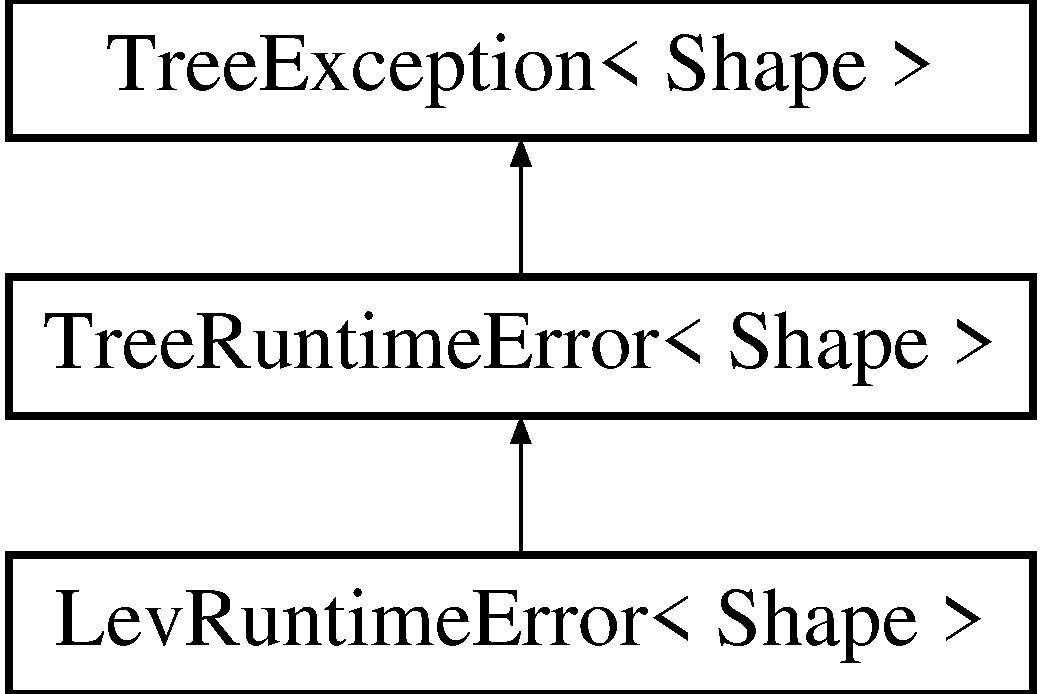
\includegraphics[height=3cm]{classTreeRuntimeError}
\end{center}
\end{figure}


\subsection{Detailed Description}
\subsubsection*{template$<$class Shape$>$ class TreeRuntimeError$<$ Shape $>$}

Exceptions derived from runtime\_\-error are provided to report events that are beyond the scope of a program and are not easily avoidable. 

The documentation for this class was generated from the following file:\begin{DoxyCompactItemize}
\item 
src/\hyperlink{exception__handling_8hpp}{exception\_\-handling.hpp}\end{DoxyCompactItemize}

\hypertarget{classTriangle}{
\section{Triangle$<$ NNODES $>$ Class Template Reference}
\label{classTriangle}\index{Triangle@{Triangle}}
}


This class implements a \hyperlink{classTriangle}{Triangle} as an objects composed by three or six nodes.  


{\ttfamily \#include $<$mesh\_\-objects.hpp$>$}Inheritance diagram for Triangle$<$ NNODES $>$::\begin{figure}[H]
\begin{center}
\leavevmode
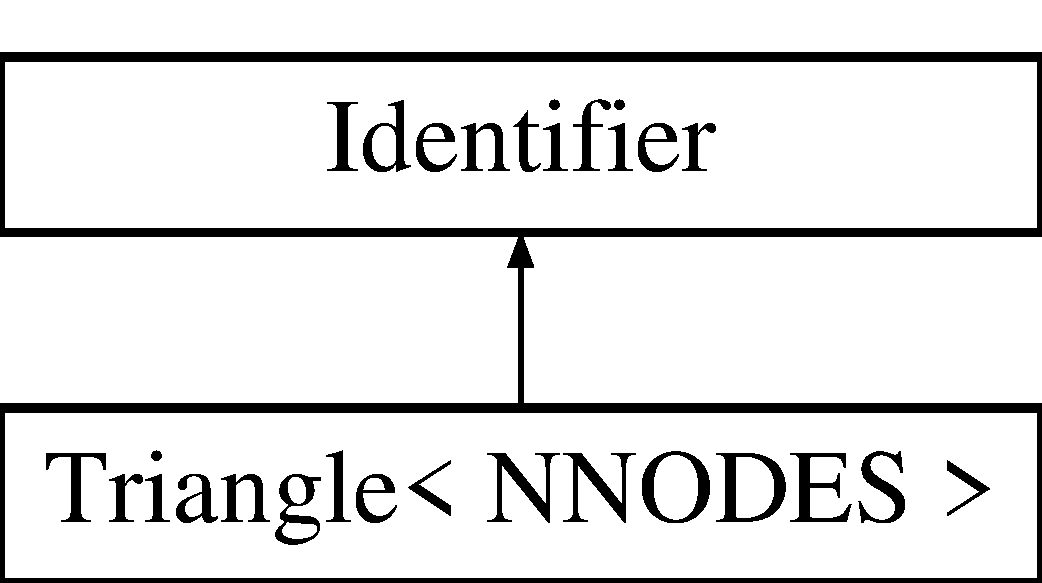
\includegraphics[height=2cm]{classTriangle}
\end{center}
\end{figure}
\subsection*{Public Member Functions}
\begin{DoxyCompactItemize}
\item 
\hypertarget{classTriangle_a1f52e8639c742a110d65ea909c408f48}{
\hyperlink{classTriangle_a1f52e8639c742a110d65ea909c408f48}{Triangle} ()}
\label{classTriangle_a1f52e8639c742a110d65ea909c408f48}

\begin{DoxyCompactList}\small\item\em This constructor creates an \char`\"{}empty\char`\"{} \hyperlink{classTriangle}{Triangle}, with an Id Not Valid. \item\end{DoxyCompactList}\item 
\hypertarget{classTriangle_a97691f5a22b40e10a8e8f49474e467be}{
\hyperlink{classTriangle_a97691f5a22b40e10a8e8f49474e467be}{Triangle} (Id id, const std::vector$<$ \hyperlink{classPoint}{Point} $>$ \&points)}
\label{classTriangle_a97691f5a22b40e10a8e8f49474e467be}

\begin{DoxyCompactList}\small\item\em This constructor creates a \hyperlink{classTriangle}{Triangle}, given its Id and an std array with the three object \hyperlink{classPoint}{Point} the will define the \hyperlink{classTriangle}{Triangle}. \item\end{DoxyCompactList}\item 
\hypertarget{classTriangle_a3be310ba8e6304749d998d0ca304752c}{
\hyperlink{classTriangle_a3be310ba8e6304749d998d0ca304752c}{Triangle} (const std::vector$<$ Real $>$ \&points)}
\label{classTriangle_a3be310ba8e6304749d998d0ca304752c}

\begin{DoxyCompactList}\small\item\em This constructor creates a \hyperlink{classTriangle}{Triangle}, given its a std::vector with six coordinate of the three point that will define the \hyperlink{classTriangle}{Triangle} (x1,y1,x2,y2,x3,y3), it's necessary for communicate with \hyperlink{classADTree}{ADTree} structure. \item\end{DoxyCompactList}\item 
\hyperlink{classPoint}{Point} \hyperlink{classTriangle_a4f2a08d6e79d0992cb23938d0fece62c}{operator\mbox{[}$\,$\mbox{]}} (UInt i) const 
\begin{DoxyCompactList}\small\item\em Overloading of the operator \mbox{[}\mbox{]}, taking the Node number and returning a node as \hyperlink{classPoint}{Point} object. \item\end{DoxyCompactList}\item 
Real \hyperlink{classTriangle_afd08dcbf5895b0c7cba20f296d40c068}{getDetJ} () const 
\begin{DoxyCompactList}\small\item\em A member that computes the barycentric coordinates. \item\end{DoxyCompactList}\item 
\hypertarget{classTriangle_abeb0bdaf6cebe42380bb80b8539a86d2}{
Eigen::Matrix$<$ Real, 2, 2 $>$ {\bfseries getM\_\-J} () const }
\label{classTriangle_abeb0bdaf6cebe42380bb80b8539a86d2}

\item 
\hypertarget{classTriangle_a93dd8dda1091b4e05d16da8d562bfcd0}{
Eigen::Matrix$<$ Real, 2, 2 $>$ {\bfseries getM\_\-invJ} () const }
\label{classTriangle_a93dd8dda1091b4e05d16da8d562bfcd0}

\item 
\hypertarget{classTriangle_acc9587525640ef364409f554a69aa3f7}{
Eigen::Matrix$<$ Real, 2, 2 $>$ {\bfseries getMetric} () const }
\label{classTriangle_acc9587525640ef364409f554a69aa3f7}

\item 
Real \hyperlink{classTriangle_a319c68c604089e6de23459d8c6d52f8a}{getArea} () const 
\begin{DoxyCompactList}\small\item\em A member returning the area of the finite element. \item\end{DoxyCompactList}\item 
\hypertarget{classTriangle_ae35c765865d38ad7323b5615cd9bbfe4}{
Eigen::Matrix$<$ Real, 3, 1 $>$ {\bfseries getBaryCoordinates} (const \hyperlink{classPoint}{Point} \&point) const }
\label{classTriangle_ae35c765865d38ad7323b5615cd9bbfe4}

\item 
bool \hyperlink{classTriangle_a76c1691d2b89f8aef8913b0315371429}{isPointInside} (const \hyperlink{classPoint}{Point} \&point) const 
\begin{DoxyCompactList}\small\item\em A member that tests if a \hyperlink{classPoint}{Point} is located inside a \hyperlink{classTriangle}{Triangle}. \item\end{DoxyCompactList}\item 
int \hyperlink{classTriangle_ad9d72fba98eaa955fca0ebc08584ee27}{getPointDirection} (const \hyperlink{classPoint}{Point} \&point) const 
\begin{DoxyCompactList}\small\item\em A memeber that verifies which edge separates the \hyperlink{classTriangle}{Triangle} from a \hyperlink{classPoint}{Point}. \item\end{DoxyCompactList}\item 
void \hyperlink{classTriangle_a083c32066c8c469e3e0f622ed4ce3e8a}{print} (std::ostream \&out) const 
\begin{DoxyCompactList}\small\item\em A member that prints the main properties of the triangle. \item\end{DoxyCompactList}\end{DoxyCompactItemize}
\subsection*{Static Public Member Functions}
\begin{DoxyCompactItemize}
\item 
\hypertarget{classTriangle_acf8960ec24710c9ec36de3b0d215e607}{
static constexpr int \hyperlink{classTriangle_acf8960ec24710c9ec36de3b0d215e607}{dp} ()}
\label{classTriangle_acf8960ec24710c9ec36de3b0d215e607}

\begin{DoxyCompactList}\small\item\em Returns the number of physical space dimension. \item\end{DoxyCompactList}\item 
\hypertarget{classTriangle_a13e45a6ea1f8d08dfe11f731b8625971}{
static constexpr int \hyperlink{classTriangle_a13e45a6ea1f8d08dfe11f731b8625971}{dt} ()}
\label{classTriangle_a13e45a6ea1f8d08dfe11f731b8625971}

\begin{DoxyCompactList}\small\item\em Returns the number of dimensions used for the search (2$\ast$2). \item\end{DoxyCompactList}\item 
\hypertarget{classTriangle_a3b983936120f9167a549fc2044a04adb}{
static constexpr int \hyperlink{classTriangle_a3b983936120f9167a549fc2044a04adb}{coordsize} ()}
\label{classTriangle_a3b983936120f9167a549fc2044a04adb}

\begin{DoxyCompactList}\small\item\em Returns the size of coordinate array. \item\end{DoxyCompactList}\end{DoxyCompactItemize}
\subsection*{Static Public Attributes}
\begin{DoxyCompactItemize}
\item 
\hypertarget{classTriangle_a235d77391422024ac15a53155d957116}{
static const UInt {\bfseries numVertices} = 3}
\label{classTriangle_a235d77391422024ac15a53155d957116}

\item 
\hypertarget{classTriangle_a3da7e9001c7ecf58fd02c237a31df732}{
static const UInt {\bfseries numSides} = 3}
\label{classTriangle_a3da7e9001c7ecf58fd02c237a31df732}

\item 
\hypertarget{classTriangle_a09b9dea67585d95f1e4b573922a9f79d}{
static const UInt {\bfseries myDim} = 2}
\label{classTriangle_a09b9dea67585d95f1e4b573922a9f79d}

\end{DoxyCompactItemize}


\subsection{Detailed Description}
\subsubsection*{template$<$UInt NNODES$>$ class Triangle$<$ NNODES $>$}

This class implements a \hyperlink{classTriangle}{Triangle} as an objects composed by three or six nodes. The first three nodes represent the vertices, the others the internal nodes, following this enumeration: !IMPORTANT! different from Sangalli code!

3 $\ast$ / $\backslash$ 5 $\ast$ $\ast$ 4 / $\backslash$ $\ast$\_\-\_\-\_\-\_\-\_\-\_\-$\ast$\_\-\_\-\_\-\_\-\_\-\_\-$\ast$ 1 6 2

the coordinates usefull for point location are the first three, so I always use 0,1,2 index independently if the class has three or six nodes! is only a 2D triangle, so the correspondig bounding box must have NDIMP = 2 

\subsection{Member Function Documentation}
\hypertarget{classTriangle_a319c68c604089e6de23459d8c6d52f8a}{
\index{Triangle@{Triangle}!getArea@{getArea}}
\index{getArea@{getArea}!Triangle@{Triangle}}
\subsubsection[{getArea}]{\setlength{\rightskip}{0pt plus 5cm}template$<$UInt NNODES$>$ Real {\bf Triangle}$<$ NNODES $>$::getArea () const\hspace{0.3cm}{\ttfamily  \mbox{[}inline\mbox{]}}}}
\label{classTriangle_a319c68c604089e6de23459d8c6d52f8a}


A member returning the area of the finite element. \begin{DoxyReturn}{Returns}
a Real value representing the area of the triangle from which we updated the element 
\end{DoxyReturn}
\begin{DoxySeeAlso}{See also}
updateElement(Triangle$<$Integrator::NNODES$>$ t) 
\end{DoxySeeAlso}
\hypertarget{classTriangle_afd08dcbf5895b0c7cba20f296d40c068}{
\index{Triangle@{Triangle}!getDetJ@{getDetJ}}
\index{getDetJ@{getDetJ}!Triangle@{Triangle}}
\subsubsection[{getDetJ}]{\setlength{\rightskip}{0pt plus 5cm}template$<$UInt NNODES$>$ Real {\bf Triangle}$<$ NNODES $>$::getDetJ () const\hspace{0.3cm}{\ttfamily  \mbox{[}inline\mbox{]}}}}
\label{classTriangle_afd08dcbf5895b0c7cba20f296d40c068}


A member that computes the barycentric coordinates. 
\begin{DoxyParams}{Parameters}
\item[{\em point}]a \hyperlink{classPoint}{Point} object \end{DoxyParams}
\begin{DoxyReturn}{Returns}
The three baricentric coordinates of the point 
\end{DoxyReturn}
\hypertarget{classTriangle_ad9d72fba98eaa955fca0ebc08584ee27}{
\index{Triangle@{Triangle}!getPointDirection@{getPointDirection}}
\index{getPointDirection@{getPointDirection}!Triangle@{Triangle}}
\subsubsection[{getPointDirection}]{\setlength{\rightskip}{0pt plus 5cm}template$<$UInt NNODES$>$ int {\bf Triangle}$<$ NNODES $>$::getPointDirection (const {\bf Point} \& {\em point}) const\hspace{0.3cm}{\ttfamily  \mbox{[}inline\mbox{]}}}}
\label{classTriangle_ad9d72fba98eaa955fca0ebc08584ee27}


A memeber that verifies which edge separates the \hyperlink{classTriangle}{Triangle} from a \hyperlink{classPoint}{Point}. 
\begin{DoxyParams}{Parameters}
\item[{\em point}]a \hyperlink{classPoint}{Point} object. \end{DoxyParams}
\begin{DoxyReturn}{Returns}
The number of the \hyperlink{classEdge}{Edge} that separates the point from the triangle and -\/1 if the point is inside the triangle. 
\end{DoxyReturn}
\hypertarget{classTriangle_a76c1691d2b89f8aef8913b0315371429}{
\index{Triangle@{Triangle}!isPointInside@{isPointInside}}
\index{isPointInside@{isPointInside}!Triangle@{Triangle}}
\subsubsection[{isPointInside}]{\setlength{\rightskip}{0pt plus 5cm}template$<$UInt NNODES$>$ bool {\bf Triangle}$<$ NNODES $>$::isPointInside (const {\bf Point} \& {\em point}) const\hspace{0.3cm}{\ttfamily  \mbox{[}inline\mbox{]}}}}
\label{classTriangle_a76c1691d2b89f8aef8913b0315371429}


A member that tests if a \hyperlink{classPoint}{Point} is located inside a \hyperlink{classTriangle}{Triangle}. 
\begin{DoxyParams}{Parameters}
\item[{\em point}]a \hyperlink{classPoint}{Point} object. \end{DoxyParams}
\begin{DoxyReturn}{Returns}
True if the point is inside the triangle 
\end{DoxyReturn}
\hypertarget{classTriangle_a4f2a08d6e79d0992cb23938d0fece62c}{
\index{Triangle@{Triangle}!operator\mbox{[}\mbox{]}@{operator[]}}
\index{operator\mbox{[}\mbox{]}@{operator[]}!Triangle@{Triangle}}
\subsubsection[{operator[]}]{\setlength{\rightskip}{0pt plus 5cm}template$<$UInt NNODES$>$ {\bf Point} {\bf Triangle}$<$ NNODES $>$::operator\mbox{[}$\,$\mbox{]} (UInt {\em i}) const\hspace{0.3cm}{\ttfamily  \mbox{[}inline\mbox{]}}}}
\label{classTriangle_a4f2a08d6e79d0992cb23938d0fece62c}


Overloading of the operator \mbox{[}\mbox{]}, taking the Node number and returning a node as \hyperlink{classPoint}{Point} object. For node numbering convention see: 
\begin{DoxyParams}{Parameters}
\item[{\em i}]an integer argument. \end{DoxyParams}
\begin{DoxyReturn}{Returns}
the \hyperlink{classPoint}{Point} object 
\end{DoxyReturn}
\hypertarget{classTriangle_a083c32066c8c469e3e0f622ed4ce3e8a}{
\index{Triangle@{Triangle}!print@{print}}
\index{print@{print}!Triangle@{Triangle}}
\subsubsection[{print}]{\setlength{\rightskip}{0pt plus 5cm}template$<$UInt NNODES$>$ void {\bf Triangle}$<$ NNODES $>$::print (std::ostream \& {\em out}) const\hspace{0.3cm}{\ttfamily  \mbox{[}inline\mbox{]}}}}
\label{classTriangle_a083c32066c8c469e3e0f622ed4ce3e8a}


A member that prints the main properties of the triangle. 
\begin{DoxyParams}{Parameters}
\item[{\em out}]a std::outstream. \end{DoxyParams}


The documentation for this class was generated from the following files:\begin{DoxyCompactItemize}
\item 
src/mesh\_\-objects.hpp\item 
src/mesh\_\-objects\_\-imp.hpp\end{DoxyCompactItemize}

\hypertarget{structtriangulateio}{
\section{triangulateio Struct Reference}
\label{structtriangulateio}\index{triangulateio@{triangulateio}}
}
\subsection*{Public Attributes}
\begin{DoxyCompactItemize}
\item 
\hypertarget{structtriangulateio_a601d8261e3e18cd0d4771730ab2172b2}{
TRIREAL $\ast$ {\bfseries pointlist}}
\label{structtriangulateio_a601d8261e3e18cd0d4771730ab2172b2}

\item 
\hypertarget{structtriangulateio_a83e7fd743b37606594ff63caddf920d0}{
TRIREAL $\ast$ {\bfseries pointattributelist}}
\label{structtriangulateio_a83e7fd743b37606594ff63caddf920d0}

\item 
\hypertarget{structtriangulateio_acb2a9792412a2c3051fb869e88cfa602}{
int $\ast$ {\bfseries pointmarkerlist}}
\label{structtriangulateio_acb2a9792412a2c3051fb869e88cfa602}

\item 
\hypertarget{structtriangulateio_a29be46ad3fc4f8c84235e420f7e606ec}{
int {\bfseries numberofpoints}}
\label{structtriangulateio_a29be46ad3fc4f8c84235e420f7e606ec}

\item 
\hypertarget{structtriangulateio_aaac6a34f7d7bf1d1476ce7672f15d976}{
int {\bfseries numberofpointattributes}}
\label{structtriangulateio_aaac6a34f7d7bf1d1476ce7672f15d976}

\item 
\hypertarget{structtriangulateio_a7d0f1c11cd6dc624ae61dbbbcc68b8cb}{
int $\ast$ {\bfseries trianglelist}}
\label{structtriangulateio_a7d0f1c11cd6dc624ae61dbbbcc68b8cb}

\item 
\hypertarget{structtriangulateio_ae73c28f6832b85cf62a97ed68ea73e7c}{
TRIREAL $\ast$ {\bfseries triangleattributelist}}
\label{structtriangulateio_ae73c28f6832b85cf62a97ed68ea73e7c}

\item 
\hypertarget{structtriangulateio_aaec63d04839bd64dc779245e2b011fa4}{
TRIREAL $\ast$ {\bfseries trianglearealist}}
\label{structtriangulateio_aaec63d04839bd64dc779245e2b011fa4}

\item 
\hypertarget{structtriangulateio_a266c62c74f443a4a50c986ccf97e74c7}{
int $\ast$ {\bfseries neighborlist}}
\label{structtriangulateio_a266c62c74f443a4a50c986ccf97e74c7}

\item 
\hypertarget{structtriangulateio_a6455c22dba63bdb0584d44fdf35a321f}{
int {\bfseries numberoftriangles}}
\label{structtriangulateio_a6455c22dba63bdb0584d44fdf35a321f}

\item 
\hypertarget{structtriangulateio_aaeeda011ca1f51696fcc5a460b81c18d}{
int {\bfseries numberofcorners}}
\label{structtriangulateio_aaeeda011ca1f51696fcc5a460b81c18d}

\item 
\hypertarget{structtriangulateio_a272ba3b8730997b1bd6c367328b1abf8}{
int {\bfseries numberoftriangleattributes}}
\label{structtriangulateio_a272ba3b8730997b1bd6c367328b1abf8}

\item 
\hypertarget{structtriangulateio_ad45fec0a70058760450e09b949a3d1c0}{
int $\ast$ {\bfseries segmentlist}}
\label{structtriangulateio_ad45fec0a70058760450e09b949a3d1c0}

\item 
\hypertarget{structtriangulateio_a8d88affa03ad1156b1d087448166bf04}{
int $\ast$ {\bfseries segmentmarkerlist}}
\label{structtriangulateio_a8d88affa03ad1156b1d087448166bf04}

\item 
\hypertarget{structtriangulateio_a417da9cc4711390560c6af7750d13d95}{
int {\bfseries numberofsegments}}
\label{structtriangulateio_a417da9cc4711390560c6af7750d13d95}

\item 
\hypertarget{structtriangulateio_a7f96a1630b7461f520f5e4f00c2d1874}{
TRIREAL $\ast$ {\bfseries holelist}}
\label{structtriangulateio_a7f96a1630b7461f520f5e4f00c2d1874}

\item 
\hypertarget{structtriangulateio_a91deb1af3dd2ef937f1b6b7e38261e99}{
int {\bfseries numberofholes}}
\label{structtriangulateio_a91deb1af3dd2ef937f1b6b7e38261e99}

\item 
\hypertarget{structtriangulateio_aa2d3a0237738f5f6cb09476ab007358d}{
TRIREAL $\ast$ {\bfseries regionlist}}
\label{structtriangulateio_aa2d3a0237738f5f6cb09476ab007358d}

\item 
\hypertarget{structtriangulateio_ac1082ccae35526598ba0977068da9278}{
int {\bfseries numberofregions}}
\label{structtriangulateio_ac1082ccae35526598ba0977068da9278}

\item 
\hypertarget{structtriangulateio_af8374f90431a318b694bb5424814f111}{
int $\ast$ {\bfseries edgelist}}
\label{structtriangulateio_af8374f90431a318b694bb5424814f111}

\item 
\hypertarget{structtriangulateio_a3f9be953734099d409f54736c3cd72af}{
int $\ast$ {\bfseries edgemarkerlist}}
\label{structtriangulateio_a3f9be953734099d409f54736c3cd72af}

\item 
\hypertarget{structtriangulateio_a0b1c374976e8352386ee4f4ac4b4fcff}{
TRIREAL $\ast$ {\bfseries normlist}}
\label{structtriangulateio_a0b1c374976e8352386ee4f4ac4b4fcff}

\item 
\hypertarget{structtriangulateio_ac8c1b394861ed4a5c021a2d08a36a2a9}{
int {\bfseries numberofedges}}
\label{structtriangulateio_ac8c1b394861ed4a5c021a2d08a36a2a9}

\end{DoxyCompactItemize}


The documentation for this struct was generated from the following file:\begin{DoxyCompactItemize}
\item 
src/triangle.h\end{DoxyCompactItemize}

\chapter{File Documentation}
\hypertarget{adtree_8hpp}{
\section{src/adtree.hpp File Reference}
\label{adtree_8hpp}\index{src/adtree.hpp@{src/adtree.hpp}}
}
{\ttfamily \#include \char`\"{}FEMr.hpp\char`\"{}}\par
{\ttfamily \#include \char`\"{}tree\_\-header.hpp\char`\"{}}\par
{\ttfamily \#include \char`\"{}mesh\_\-objects.hpp\char`\"{}}\par
{\ttfamily \#include \char`\"{}bounding\_\-box.hpp\char`\"{}}\par
{\ttfamily \#include \char`\"{}domain.hpp\char`\"{}}\par
{\ttfamily \#include \char`\"{}treenode.hpp\char`\"{}}\par
{\ttfamily \#include \char`\"{}exception\_\-handling.hpp\char`\"{}}\par
{\ttfamily \#include \char`\"{}adtree\_\-imp.hpp\char`\"{}}\par
\subsection*{Classes}
\begin{DoxyCompactItemize}
\item 
class \hyperlink{classADTree}{ADTree$<$ Shape $>$}
\begin{DoxyCompactList}\small\item\em Alternating binary range searching tree. \item\end{DoxyCompactList}\end{DoxyCompactItemize}


\subsection{Detailed Description}
\begin{DoxyAuthor}{Author}
Cardani Alessandra 

Pigoli Davide 

Prada Daniele 
\end{DoxyAuthor}

\hypertarget{domain_8hpp}{
\section{src/domain.hpp File Reference}
\label{domain_8hpp}\index{src/domain.hpp@{src/domain.hpp}}
}
{\ttfamily \#include \char`\"{}FEMr.hpp\char`\"{}}\par
{\ttfamily \#include \char`\"{}domain\_\-imp.hpp\char`\"{}}\par
\subsection*{Classes}
\begin{DoxyCompactItemize}
\item 
class \hyperlink{classDomain}{Domain$<$ Shape $>$}
\begin{DoxyCompactList}\small\item\em It defines geometric limits of a set of points. template parameter Shape is the original geometric figure (ex: triangle, box), it's useful to extract the physical dimension. \item\end{DoxyCompactList}\end{DoxyCompactItemize}


\subsection{Detailed Description}
\begin{DoxyAuthor}{Author}
Alessandra Cardani 

Pigoli Davide 

Prada Daniele 
\end{DoxyAuthor}

\hypertarget{exception__handling_8hpp}{
\section{src/exception\_\-handling.hpp File Reference}
\label{exception__handling_8hpp}\index{src/exception\_\-handling.hpp@{src/exception\_\-handling.hpp}}
}
{\ttfamily \#include \char`\"{}FEMr.hpp\char`\"{}}\par
{\ttfamily \#include \char`\"{}mesh\_\-objects.hpp\char`\"{}}\par
{\ttfamily \#include \char`\"{}bounding\_\-box.hpp\char`\"{}}\par
\subsection*{Classes}
\begin{DoxyCompactItemize}
\item 
class \hyperlink{classTreeException}{TreeException$<$ Shape $>$}
\item 
class \hyperlink{classTreeLogicError}{TreeLogicError$<$ Shape $>$}
\item 
class \hyperlink{classTreeAlloc}{TreeAlloc$<$ Shape $>$}
\item 
class \hyperlink{classTreeDomainError}{TreeDomainError$<$ Shape $>$}
\item 
class \hyperlink{classTreeLengthError}{TreeLengthError$<$ Shape $>$}
\item 
class \hyperlink{classLocLengthError}{LocLengthError$<$ Shape $>$}
\begin{DoxyCompactList}\small\item\em This class is used to report an attempt to build a tree with more memory locations than a fixed limit. \item\end{DoxyCompactList}\item 
class \hyperlink{classTreeRuntimeError}{TreeRuntimeError$<$ Shape $>$}
\item 
class \hyperlink{classLevRuntimeError}{LevRuntimeError$<$ Shape $>$}
\begin{DoxyCompactList}\small\item\em This class is used to report an attempt to build a tree with more levels than a fixed limit. \item\end{DoxyCompactList}\end{DoxyCompactItemize}
\subsection*{Functions}
\begin{DoxyCompactItemize}
\item 
\hypertarget{exception__handling_8hpp_a908d4e9a617ddcbb6c8a213fb5997d16}{
{\footnotesize template$<$class Shape $>$ }\\std::ostream \& {\bfseries operator$<$$<$} (std::ostream \&ostr, \hyperlink{classTreeDomainError}{TreeDomainError}$<$ Shape $>$ const \&de)}
\label{exception__handling_8hpp_a908d4e9a617ddcbb6c8a213fb5997d16}

\end{DoxyCompactItemize}


\subsection{Detailed Description}
\begin{DoxyAuthor}{Author}
Cardani Alessandra 

Pigoli Davide 

Prada Daniele 
\end{DoxyAuthor}

\hypertarget{tree__header_8hpp}{
\section{src/tree\_\-header.hpp File Reference}
\label{tree__header_8hpp}\index{src/tree\_\-header.hpp@{src/tree\_\-header.hpp}}
}
{\ttfamily \#include \char`\"{}FEMr.hpp\char`\"{}}\par
{\ttfamily \#include \char`\"{}mesh\_\-objects.hpp\char`\"{}}\par
{\ttfamily \#include \char`\"{}bounding\_\-box.hpp\char`\"{}}\par
{\ttfamily \#include \char`\"{}domain.hpp\char`\"{}}\par
{\ttfamily \#include \char`\"{}treenode.hpp\char`\"{}}\par
{\ttfamily \#include \char`\"{}exception\_\-handling.hpp\char`\"{}}\par
{\ttfamily \#include \char`\"{}tree\_\-header\_\-imp.hpp\char`\"{}}\par
\subsection*{Classes}
\begin{DoxyCompactItemize}
\item 
class \hyperlink{classTree__Header}{Tree\_\-Header$<$ T $>$}
\end{DoxyCompactItemize}


\subsection{Detailed Description}
\begin{DoxyAuthor}{Author}
Cardani Alessandra 

Pigoli Davide 

Prada Daniele 
\end{DoxyAuthor}

\hypertarget{treenode_8hpp}{
\section{src/treenode.hpp File Reference}
\label{treenode_8hpp}\index{src/treenode.hpp@{src/treenode.hpp}}
}
{\ttfamily \#include \char`\"{}FEMr.hpp\char`\"{}}\par
{\ttfamily \#include \char`\"{}treenode\_\-imp.hpp\char`\"{}}\par
\subsection*{Classes}
\begin{DoxyCompactItemize}
\item 
class \hyperlink{classTreeNode}{TreeNode$<$ Shape $>$}
\begin{DoxyCompactList}\small\item\em Class defining a tree node. \item\end{DoxyCompactList}\end{DoxyCompactItemize}


\subsection{Detailed Description}
\begin{DoxyAuthor}{Author}
Alessandra Cardani 

Pigoli Davide 

Prada Daniele 
\end{DoxyAuthor}

\printindex
\end{document}
